\documentclass[phd,tocprelim,dvipsnames]{cornell}
\usepackage[utf8]{inputenc}
\usepackage{graphicx,pstricks}
\usepackage{graphics}
\usepackage{subfigure}
\usepackage{palatino}
\usepackage{natbib}
\usepackage{color}
\usepackage{amsmath,amsthm,amsbsy,verbatim,amssymb,amsfonts,amscd,mathrsfs}
\usepackage{algorithm}
\usepackage[algo2e,ruled,algochapter]{algorithm2e}
\usepackage[hidelinks]{hyperref}
\usepackage[capitalise]{cleveref}
\usepackage[inline]{enumitem}  % Horizontal lists
\usepackage{mathtools}  % for overbracket
\usepackage{booktabs}  % for professional tables
\usepackage{multirow}	 % for multi-rows and columns
\usepackage{makecell}  % thead, other vertical alignment options
\usepackage{hhline}  % double horizontal lines for tables
\usepackage{longtable}  % long tables
\usepackage{minted}  % for code examples
\usepackage[most]{tcolorbox}  % boxes around code examples
\usepackage{etoolbox}  % more minted customizing
\usepackage{amsbsy}  % For bold script


%%%%%%%%%%%%%% Custom comments stuff
\newif\ifcomments
%\commentsfalse
\commentstrue
\ifcomments\newcommand{\comments}[1]{#1}\else\newcommand{\comments}[1]{}\fi
\definecolor{clrgp}{rgb}{.9,0,.9}
\definecolor{green}{rgb}{0,0.5,0}
\newcommand{\gp}[1]{\comments{\textcolor{clrgp}{[GP: #1]}}}


%%%%%%%%%%%%%% Formatting
\bibliographystyle{plainnat}
\renewcommand{\cite}[1]{\citep{#1}}
\renewcommand{\topfraction}{0.85}
\renewcommand{\textfraction}{0.1}
\renewcommand{\floatpagefraction}{0.75}
\addtolength{\skip\footins}{2pc plus 5pt} % Footnote spacing
%if you're having problems with overfull boxes, you may need to increase
%the tolerance to 9999
\tolerance=9999


%%%%%%%%%%%%% Special characters
\DeclareUnicodeCharacter{00D7}{\texttimes}


%%%%%%%%%%%%% Algorithms
\newlength\inputlen


%%%%%%%%%%%%% Enumeration style
\setlist[enumerate]{font={\bfseries}}% global settings, for all lists
\setlist[enumerate,1]{label={(\arabic*)}}


%%%%%%%%%%%%% Code examples
\newif\iflongcode
\longcodefalse
\BeforeBeginEnvironment{minted}{%
  \iflongcode
    \begin{tcolorbox}[enhanced,breakable]
  \else
    \begin{tcolorbox}
  \fi
    \singlespacing
    \footnotesize
}
\AfterEndEnvironment{minted}{%
  \end{tcolorbox}
}


%%%%%%%%%%%%% For too large figures/tables
% https://tex.stackexchange.com/questions/16582/center-figure-that-is-wider-than-textwidth
\makeatletter
\newcommand*{\centerfloat}{%
  \parindent \z@
  \leftskip \z@ \@plus 1fil \@minus \textwidth
  \rightskip\leftskip
  \parfillskip \z@skip}
\makeatother


%%%%%%%%%%%%%% Theorems, observations, etc.
\newtheorem{observation}{Observation}[chapter]
\newtheorem{property}{Property}[chapter]
\newtheorem{theorem}{Theorem}[chapter]
\newtheorem{corollary}{Corollary}[chapter]
\newtheorem{lemma}{Lemma}[chapter]


%%%%%%%%%%%%%% Autoref
\renewcommand{\chapterautorefname}{Chapter}
\renewcommand{\sectionautorefname}{Section}
\renewcommand{\subsectionautorefname}{Section}
\renewcommand{\algorithmautorefname}{Algorithm}
\newcommand{\definitionautorefname}{Definition}
\newcommand{\observationautorefname}{Observation}
\newcommand{\propertyautorefname}{Property}
\newcommand{\thmautorefname}{Theorem}
\newcommand{\lemmaautorefname}{Lemma}
\newcommand\numberthis{\addtocounter{equation}{1}\tag{\theequation}}


%%%%%%%%%%%%%% Macros
\DeclareMathOperator*{\argmax}{arg\,max}
\DeclareMathOperator*{\argmin}{arg\,min}
\DeclareMathOperator*{\expectedvalue}{\mathbb{E}}
\DeclareMathOperator*{\variance}{Var}
\DeclareMathOperator*{\covariance}{Cov}
\DeclareMathOperator*{\trace}{Tr}

% Probability
\newcommand{\bigo}[1]{\ensuremath{\mathchoice{\mathcal O \! \left( #1 \right)}}{\mathcal O ( #1 )}{}{}}
\newcommand{\bigomega}[1]{\ensuremath{\mathchoice{\Omega \! \left( #1 \right)}}{\Omega ( #1 )}{}{}}
\newcommand{\ints}{\ensuremath{\mathbb{Z}}}
\newcommand{\reals}{\ensuremath{\mathbb{R}}}
\newcommand{\GP}[2]{\ensuremath{\mathcal{GP} \left[ #1, #2 \right]}}
\newcommand{\normaldist}[2]{\ensuremath{\mathcal{N} \left[ #1, #2 \right]}}
\renewcommand{\Pr}[1]{\ensuremath{\text{Pr} \left[ #1 \right]}}
\newcommand{\Ev}[1]{\ensuremath{\expectedvalue \left[ #1 \right]}}
\newcommand{\Evover}[2]{\ensuremath{\expectedvalue_{#1} \left[ #2 \right]}}
\newcommand{\Var}[1]{\ensuremath{\variance \left[ #1 \right]}}
\newcommand{\Varover}[2]{\ensuremath{\variance_{#1} \left[ #2 \right]}}
\newcommand{\Cov}[1]{\ensuremath{\covariance \left[ #1 \right]}}
\newcommand{\Covover}[2]{\ensuremath{\covariance_{#1} \left[ #2 \right]}}
\newcommand{\given}{\mid}

% Other matrix/math operators
\newcommand{\tr}[1]{\ensuremath{\mathchoice{\trace \left( #1 \right)}{\trace ( #1 )}{}{}}}
\newcommand{\inv}{^{-1}}
\newcommand{\trans}{^{\top}}
\newcommand{\intd}[1]{\,\mathrm{d}{#1}}

% Matrices / vectors
\newif\ifboldmatrix
\boldmatrixtrue
\ifboldmatrix\newcommand{\boldmatrix}[1]{\mathbf{#1}}\else\newcommand{\boldmatrix}[1]{#1}\fi
\newcommand{\ba}{\ensuremath{\mathbf{a}}}
\newcommand{\bb}{\ensuremath{\mathbf{b}}}
\newcommand{\bd}{\ensuremath{\mathbf{d}}}
\newcommand{\be}{\ensuremath{\mathbf{e}}}
\newcommand{\bfn}{\ensuremath{\mathbf{f}}}
\newcommand{\bk}{\ensuremath{\mathbf{k}}}
\newcommand{\bm}{\ensuremath{\mathbf{m}}}
\newcommand{\bmu}{\ensuremath{\boldsymbol{\mu}}}
\newcommand{\bp}{\ensuremath{\mathbf{p}}}
\newcommand{\bq}{\ensuremath{\mathbf{q}}}
\newcommand{\br}{\ensuremath{\mathbf{r}}}
\newcommand{\bs}{\ensuremath{\mathbf{s}}}
\newcommand{\bt}{\ensuremath{\mathbf{t}}}
\newcommand{\btheta}{\ensuremath{\boldsymbol{\theta}}}
\newcommand{\bu}{\ensuremath{\mathbf{u}}}
\newcommand{\bv}{\ensuremath{\mathbf{v}}}
\newcommand{\bw}{\ensuremath{\mathbf{w}}}
\newcommand{\bx}{\ensuremath{\mathbf{x}}}
\newcommand{\by}{\ensuremath{\mathbf{y}}}
\newcommand{\bz}{\ensuremath{\mathbf{z}}}
\newcommand{\bzero}{\ensuremath{\mathbf{0}}}
\newcommand{\bone}{\ensuremath{\mathbf{1}}}
\newcommand{\bA}{\ensuremath{\boldmatrix{A}}}
\newcommand{\bB}{\ensuremath{\boldmatrix{B}}}
\newcommand{\bC}{\ensuremath{\boldmatrix{C}}}
\newcommand{\bD}{\ensuremath{\boldmatrix{D}}}
\newcommand{\bI}{\ensuremath{\boldmatrix{I}}}
\newcommand{\bK}{\ensuremath{\boldmatrix{K}}}
\newcommand{\bL}{\ensuremath{\boldmatrix{L}}}
\newcommand{\bM}{\ensuremath{\boldmatrix{M}}}
\newcommand{\bP}{\ensuremath{\boldmatrix{P}}}
\newcommand{\bQ}{\ensuremath{\boldmatrix{Q}}}
\newcommand{\bR}{\ensuremath{\boldmatrix{R}}}
\newcommand{\bSigma}{\ensuremath{\boldsymbol{\Sigma}}}
\newcommand{\bT}{\ensuremath{\boldmatrix{T}}}
\newcommand{\bU}{\ensuremath{\boldmatrix{U}}}
\newcommand{\bV}{\ensuremath{\boldmatrix{V}}}
\newcommand{\bW}{\ensuremath{\boldmatrix{W}}}
\newcommand{\bX}{\ensuremath{\boldmatrix{X}}}
\newcommand{\bY}{\ensuremath{\boldmatrix{Y}}}
\newcommand{\bZ}{\ensuremath{\boldmatrix{Z}}}

% Constants
\newcommand{\numdata}{\ensuremath{N}}
\newcommand{\numdim}{\ensuremath{D}}
\newcommand{\numinduc}{\ensuremath{M}}

% Data/dataset specific terms
\newcommand{\bxtest}{\ensuremath{\bx^*}}
\newcommand{\bxtestprime}{\ensuremath{\bx^{*\prime}}}
\newcommand{\bXtest}{\ensuremath{\bX^*}}
\newcommand{\ytest}{\ensuremath{y^*}}
\newcommand{\ytestprime}{\ensuremath{y^{*\prime}}}
\newcommand{\bytest}{\ensuremath{\by^*}}
\newcommand{\meantest}[1]{\ensuremath{\mu^* \left( #1 \right)}}
\newcommand{\bmeantest}[1]{\ensuremath{\bmu^* \left( #1 \right)}}
\newcommand{\covtest}[1]{\ensuremath{\sigma^* \left( #1 \right)}}
\newcommand{\Covtest}[1]{\ensuremath{\bSigma^* \left( #1 \right)}}
\newcommand{\dset}{\ensuremath{\mathcal D}}
\newcommand{\model}{\ensuremath{\mathcal M}}
\newcommand{\loglik}{\ensuremath{\mathcal L}}
\newcommand{\approxK}{\ensuremath{\widetilde{\bK}_{\bX\bX}}}
\newcommand{\trainK}{\ensuremath{\widehat{\bK}_{\bX\bX}}}
\newcommand{\trainP}{\ensuremath{\widehat{\bP}}}

% Method specific terms
\newcommand{\mmm}[1]{\ensuremath{\Xi (#1)}}
\newcommand{\mvm}[1]{\ensuremath{\xi ( #1 )}}
\newcommand{\row}[1]{\ensuremath{\rho ( #1 )}}



%%%%%%%%%%%%%%%%%%%%%%%%%%%
\title{A Scalable and Flexible Framework for Gaussian Processes via Matrix-Vector Multiplication}
\author{Geoff Pleiss}
\conferraldate{May}{2020}
\degreefield{Ph.D.}
\copyrightholder{Geoff Pleiss}
\copyrightyear{2020}


%%%%%%%%%%%%%%%%%%%%%%%%%%%
\begin{document}
\maketitle
\makecopyright


\begin{abstract}
  Gaussian processes (GPs) exhibit a classic tension of many machine learning methods:
they possess desirable modelling capabilities yet suffer from important practical limitations.
In many instances, GPs are able to offer well-calibrated uncertainty estimates, interpretable predictions, and the ability to encode prior knowledge.
These properties have made them an indispensable tool for black-box optimization, time series forecasting, and high-risk applications like health care.
Despite these benefits, GPs are typically not applied to datasets with more than a few thousand data points.
This is in part due to an inference procedure that requires matrix inverses, determinants, and other expensive operations.
Moreover, specialty models often require significant implementation efforts.

This thesis aims to alleviate these practical concerns through a single simple design decision.
Taking inspiration from neural network libraries, we construct GP inference algorithms using only \emph{matrix-vector multiplications} (MVMs) and other linear operations.
This MVM-based approach simultaneously address several of these practical concerns: it reduces asymptotic complexity, effectively utilizes GPU hardware, and provides straight-forward implementations for many specialty GP models.

The chapters of this thesis each address a different aspect of Gaussian process inference.
\cref{chapter:bbmm} introduces a MVM method for training Gaussian process regression models (i.e. optimizing kernel/likelihood hyperparameters).
This approach unifies several existing methods into a highly-parallel and stable algorithm.
\cref{chapter:love} focuses on making predictions with Gaussian processes.
A memory-efficient cache, which can be computed through MVMs, significantly reduces the computation of predictive distributions.
\cref{chapter:ciq} introduces a multi-purpose MVM algorithm that can be used to draw samples from GP posteriors and perform approximate Gaussian process inference.
All three of these methods offer speedups ranging from $4\times$ to $40\times$.
Importantly, applying any of these algorithms to specialty models (e.g. multitask GPs and scalable approximations) simply requires a matrix-vector multiplication routine that exploits covariance structure afforded by the model.

The MVM methods from this thesis form the building blocks of the \href{http://github.com/cornellius-gp/gpytorch}{\tt GPyTorch} library, an open-sourced GP implementation designed for scalability and simple implementations.
In the final chapter, we evaluate GPyTorch models on several large-scale regression datasets.
Using the proposed MVM methods, we can apply exact Gaussian processes to datasets that are \emph{2 orders of magnitude larger} than what has previously been reported---up to 1 million data points.

\end{abstract}

\begin{biosketch}
  Geoff Pleiss was born and raised in the Bay Area, though his journey into machine learning did not begin until his senior year of college.
He graduated from Olin College of Engineering in 2013 with a self-designed engineering degree, specializing in applied math and computing.
After a brief stint as a software developer and consultant at Pivotal Labs in New York City, Geoff moved to Ithaca where he began his PhD work.
At Cornell, Geoff studied machine learning under the advising of Kilian Q. Weinberger.
He is currently a researcher as ASAPP Inc.

%In west Philadelphia born and raised on the playground was where I spent most of my days.
%Chillin' out maxin' relaxin' all cool and all shootin some b-ball outside of the school,
%when a couple of guys who were up to no good started making trouble in my neighborhood.
%I got in one little fight and my mom got scared.
%She said ``You're movin' with your auntie and uncle in Bel Air.''
%I begged and pleaded with her day after day but she packed my suit case and sent me on my way.
%She gave me a kiss and then she gave me my ticket.
%I put my Walkman on and said, ``I might as well kick it.''
%First class, yo this is bad---drinking orange juice out of a champagne glass.
%Is this what the people of Bel-Air living like?
%Hmm this might be alright.
%But wait I hear they're prissy, bourgeois, all that---is this the type of place that they just send this cool cat?
%I don't think so; I'll see when I get there.
%I hope they're prepared for the prince of Bel-Air.
%Well, the plane landed and when I came out there was a dude who looked like a cop standing there with my name out.
%I ain't trying to get arrested yet.
%I just got here.
%I sprang with the quickness like lightning, disappeared.
%I whistled for a cab and when it came near the license plate said fresh and it had dice in the mirror.
%If anything I could say that this cab was rare, but I thought ``Nah, forget it---Yo, homes to Bel Air.''
%I pulled up to the house about seven or eight, and I yelled to the cabbie, ``Yo homes smell ya later!''
%I looked at my kingdom; I was finally there to sit on my throne as the Prince of Bel Air.

\end{biosketch}

\begin{dedication}
  This thesis is dedicated to my parents, Mike and Chris Pleiss, who have always been my role models in science.
I cannot thank you enough for all of your love, encouragement, and support over the years.

\end{dedication}

\begin{acknowledgements}
  Your acknowledgements go here. Make sure it sits inside the brackets.

\end{acknowledgements}

\contentspage
\tablelistpage
\figurelistpage
\addcontentsline{toc}{section}{List of Algorithms}
\listofalgorithms
\newpage

\normalspacing \setcounter{page}{1} \pagenumbering{arabic}
\pagestyle{cornell} \addtolength{\parskip}{0.5\baselineskip}

\chapter{Introduction}
\label{chapter:introduction}

%Machine learning hype <- success in many different areas.
%Success in many different areas <- advances in algorithms.
%Advances of algorithms <- both in terms of raw potential and in terms of the practical.
%The best algorithms are ones that offer both potential and practicality.
%No one algorithm is perfect <- we need a quiver of different possible algorithms.

%Don't talk about advances.
%Find a lead in to discuss algorithms.

%At this point in machine learning we have several sets of algorithms.

%Questions we need to answer:
%- Why is it important to have multiple algorithms?
%- What kind of algorithms are we looking for?

%Of course, no one algorithm is good at every possible task.
%For example, on many computer vision tasks it is commonly assumed there will be some sort of convolutional layers.
%On many Kaggle competitions, a majority of winning submissions utilize random forests.
%Therefore, it is arguably good to have a variety of possible algorithms.



%Neural networks.

The past decade has witnessed a wide-scale adoption of machine learning methods across numerous application domains.
%Here we will highlight two broad categories of methodological innovation that have contributed to this surge.
This surge is due to the confluence of several factors, of which we will highlight two.
First, researchers have demonstrated the unparalleled {\bf predictive capabilities} of several machine learning algorithms.
%Models can achieve superhuman performance on complex tasks like object recognition \cite{he2016deep}, machine translation \cite{vaswani2017attention}, and strategy game-playing \cite{silver2017mastering}.
At the same time, the community has developed algorithms that are increasingly {\bf practical and easy-to-use}.
Many models can be trained rapidly on consumer-level computer hardware \cite{howard2018training}, and high-quality software frameworks enable practitioners to rapidly develop new models.
%While many other factors have contributed to the machine learning surge, we will limit our focus to these two categories.
While machine learning's predictive successes have opened up new possibilities, its new-found ease-of-use has accelerated innovation and adoption.

Arguably, the machine learning algorithms which have had the broadest impact are the ones that seamlessly offer \emph{both} predictive power and practicality.
Deep neural networks perhaps best exemplify this trend.
Recent innovations in
network architecture \citep[e.g.][]{he2016deep,vaswani2017attention,devlin2018bert,huang2019convolutional},
optimization \citep[e.g.][]{ioffe2015batch,izmailov2018averaging},
and theoretical understanding \citep[e.g.][]{keskar2016large,jacot2018neural,arora2019fine}
have led to massive performance improvements on increasingly complex datasets.
Moreover, these innovations have been complemented by
the effective use of specialty compute hardware (such as GPUs and TPUs),
the introduction of automatic differentiation \citep[e.g.][]{paszke2017automatic},
and the development of of several high-quality software implementations~\citep[e.g.][]{jia2014caffe,abadi2016tensorflow,paszke2019pytorch}.
These pragmatic advances make it easy for practitioners to experiment with new models and architectures, which has undoubtedly contributed to its profound and wide-spread successes \cite{goodfellow2016deep}.

Gradient-boosted trees have a similar powerful-yet-practical story.
Since their inception \cite{friedman2001greedy,friedman2002stochastic}, gradient boosted trees have excelled in many applications \citep[e.g.][]{richardson2007predicting,burges2010ranknet}.
The predictive power of these models is a product of several key attributes: for example, their remarkable generalization properties \citep{freund1997decision,schapire2013boosting} and their ability to handle incomplete features \cite{friedman2001greedy}.
Equally important, these models are simple and computational efficient, in large part due to specialty parallel algorithms \citep[e.g.][]{tyree2011parallel,ke2017lightgbm} and easy-to-use software implementations such as XGBoost \cite{chen2016xgboost}.
These advantages have made gradient-boosted decision trees a workhorse algorithm for many practitioners across application domains.
According to a survey collected by \citet{kaggle2019kaggle}, $75\%$ of the responding data scientists regularly use gradient-boosted decision trees and the XGBoost software.

Nevertheless, for many machine learning algorithms there is still a trade-off between predictive potential and practical limitations.
The focus of this thesis is {\bf Gaussian process models} (GPs), which perhaps best exemplify this tension.
Within the machine learning community, GPs have been well-regarded as a powerful model class with many desirable properties---such as calibrated uncertainty estimates and interpretable model priors.
Recent work on hierarchical modelling \citep[e.g.][]{damianou2013deep} and scalability \citep[e.g.][]{wilson2015kernel} have furthered their applicability to increasingly complex tasks.
However, Gaussian processes have historically been relegated to small datasets, and the tools most commonly used for inference do not effectively utilize modern compute hardware.
%Scalable approximations can remedy these concerns to some extent, yet such approximations can sometimes bias the model's predictions \cite{turner2011two,bauer2016understanding}.
%Finally, new
Using GPs requires significant implementation effort, as simple modifications like an additional output dimension might require different learning/inference procedures.
These practical considerations hinder the adoption of GPs, while also limiting researchers' abilities to rapidly-prototype and make new developments.
This thesis aims to address these limitations so that Gaussian processes can be powerful-\emph{and}-practical models.

% Even as Moore's law runs out, specialty hardware

\section{The Predictive Power of Gaussian Processes Models}

Before addressing these issues, it is worth discussing why Gaussian processes are an invaluable model class for blackbox optimization \citep[e.g.][]{snoek2012practical}, robotics \citep[e.g.][]{deisenroth2011pilco}, health care \citep[e.g.][]{schulam2015framework}, and many other domains:
\begin{enumerate}
  \item {\bf Closed-form marginalization over hypotheses.}
    Many machine learning algorithms (such as neural networks) construct a single model by optimizing over thousands or millions of parameters.
    Gaussian processes on the other hand marginalize over all possible predictive models $f(\cdot)$:
    \[
      p_\text{GP} ( y \mid \bx ) = \int_{f(\cdot)} p( y \mid \bx, f(\cdot)) \: p(f(\cdot)) \: \intd f(\cdot).
    \]
    As a result, the predictions are less prone to overfitting \cite{rasmussen2006gaussian}.

  \item {\bf Well-calibrated uncertainty estimates.}
    The output of a Gaussian process is a predictive \emph{distribution}, which incorporates both modelling uncertainty (e.g. how many different models could fit the data) and data uncertainty (e.g. how noisy are the training data).
    Consequentially, the predictive uncertainties tend to be very well calibrated to the data distribution.

  \item {\bf A flexible language for encoding prior knowledge.}
    A Gaussian process' generalization capabilities are almost entirely determined by its modelling priors.
    Crucially, GP priors directly encode functional properties---such as smoothness, periodicity, or monotonicity---rather than beliefs about certain parameters.
    These functional properties are determined by the choice of \emph{kernel function}, which can be easily composed (see \cref{sec:common_kernels}).
    With the appropriate choice of prior, it is possible to generalize on datasets with as few as 10 observations \citep[e.g.][]{rasmussen2006gaussian,gardner2017discovering}.
    %Several recent works have simplified the task of constructing appropriate kernels, either through composition \citep{duvenaud2013structure} or through differentiable learning \citep{wilson2013gaussian}.

  \item {\bf Interpretable predictions.}
    The predictions from Gaussian processes (see \cref{eqn:predictive_mean,eqn:predictive_var}) are not only expressive and powerful; they are also very intuitive.
    If we view the GP's kernel function as a similarity/distance measure between two points, then the prediction at a given point $\bx$ is simply an interpolation of nearby training points.
    The prediction's confidence interval is small when $\bx$ is close to training points, and large when $\bx$ is too far away for accurate interpolation.
\end{enumerate}
%
\noindent
These benefits are obviously applicable in the ``small data'' regime, where priors and marginalization are critical for meaningful predictive performance \cite{rasmussen2001occam}.
However, these properties also are beneficial for large datasets.
Good uncertainty estimates and interpretable predictions are increasingly desirable for large-scale machine learning models.
%GPs (with certain kernel functions) are universal approximators \cite{micchelli2006universal}, and their modelling capacity increases with the amount of available training data.
In addition, large datasets make it possible to use powerful families of covariance functions \citep{wilson2013gaussian,wilson2016deep,benton2019function} or hierarchical (``deep'') GP models \cite{wilson2016deep,salimbeni2017doubly,jankowiak2020deep}.
%This makes GPs especially powerful on big-data tasks like large-scale extrapolation \citep[e.g.][]{jankowiak2020parametric} and high-dimensional optimization \citep[e.g.][]{eriksson2019scalable}.


\section{Practical Concerns with Gaussian Processes Models}

While Gaussian processes offer great predictive potential, there are several practical issues that hinder its use, especially on larger and more complex datasets.

\subsection{Computational Complexity and Memory Requirements}
Given $N$ training data points, Gaussian process models na\"{i}vely require $\bigo{N^3}$ computation and $\bigo{N^2}$ storage.
This complexity comes from computing a $N \times N$ covariance matrix of all training data and computing several non-linear operations (see \cref{sec:gp_models}).
Historically, this has limited exact Gaussian process models to datasets with fewer than $1,\!000$ data points \cite{hensman2013gaussian}.

\subsection{Use of Modern Compute Hardware}
It is worth noting that this $\bigo{N^3}$ computational complexity is not necessarily insurmountable given modern computational hardware.
For example, some deep learning models require many more floating point operations (FLOPs) than large-scale GPs.
A 264-layer DenseNet model \cite{huang2017densely}, common on many computer vision tasks, requires $2.4 \times 10^{18}$ FLOPs to train on $1.2$ million images.
This is essentially a cubic computational requirement, and would be wholly impractical if it were not for specialty compute hardware like GPUs.
Such a model would probably require months to train on standard CPUs, yet can be trained on 8 GPUs in a matter of hours \cite{howard2018training}.

Given the effectiveness of GPU acceleration on large neural networks, one might expect similar performance for large-scale Gaussian processes.
Unfortunately, many GP implementations rely on the Cholesky factorization (see \cref{sec:gp_models}), which does not benefit as readily from modern compute hardware.
GPUs are designed for massively-parallelizable operations such as matrix-multiplication (which is the primary numerical operation of neural networks).
A matrix-multiply between two $1,\!000 \times 1,\!000$ matrices is $10,\!000$ times faster on a GPU than on a CPU!\footnote{
	As measured on a NVIDIA GTX 1070 GPU verses an 8-core Intel i7 CPU.
}
%which is why large neural networks are practical to train.
The Cholesky algorithm on the other hand is inherently sequential and affords minimal parallelization;
factorizing a $1,\!000 \times 1,\!000$ matrix is only $10$ times faster on GPU than on CPU.
This is why we cannot expect neural-network-level speedups for Cholesky-based GPs.
Moreover, the Cholesky factorization requires $\bigo{N^2}$ storage.
This amounts to a terabyte of memory for $N=1,\!000,\!000$---well beyond the capacity of most GPU clusters.

\subsection{Choosing Appropriate Approximations}
To reduce the computational and memory burden, researchers have proposed numerous methods that approximate Gaussian processes with simpler models.
Such models employ low-rank or structured approximations of the $N \times N$ matrices (see \cref{sec:approx_gps}).
Numerous advances have made these approximate methods more powerful while retaining manageable asymptotic complexities.

However, choosing a suitable approximation involves many design choices.
All approximate methods introduce hyperparameters that control the speed/accuracy trade-off, while also making assumptions that might not be well suited to certain datasets.
For example, variational approaches \citep[e.g.][]{titsias2009variational,hensman2013gaussian}---which are a popular general-purpose approximation---tend to overestimate the observational noise, leading to worse predictive uncertainties \cite{turner2011two,bauer2016understanding}.
Structured interpolation methods \cite{wilson2015kernel} alleviate these biases, yet tend to be limited to low-dimensional problems.
While some theoretical guarantees can guide these design decisions \cite{burt2019rates}, choosing a good approximate model is ultimately dataset specific and can require expert knowledge.
%Good performance often requires a large hyperparameter sweep and expert knowledge.

\subsection{Implementation and Programmability}
One compelling advantage of neural networks is their modularity.
Creating a novel neural network architecture requires significant thought and experimentation; however, \emph{implementing} new architectures requires very little software engineering effort.
Seemingly complex models like DenseNets \cite{huang2017densely} and Transformers \cite{vaswani2017attention} have surprisingly simple implementations using compositional layers.
Small modifications, such as adding an additional output dimension, often require only a single additional line of code.

Gaussian processes models on the other hand require significant implementation effort.
Often, the \emph{model} and the \emph{learning/inference procedures} are tightly coupled.
As an example, consider a Gaussian process with multiple output dimensions \cite{bonilla2008multi}.
While this model and a standard (single-output) GP are seemingly similar, they require completely different implementations.
The additional output dimension changes the structure of the prior covariance matrix (see \cref{sec:programmability}), modifying the equations used for efficient inference.
In the popular \citet{gpy2014} software package, multi-output GPs and standard GPs are implemented as separate models, with multi-output GPs requiring an additional 100 lines of code.
Compared to the one-line change for multi-output neural networks, GPs are significantly more difficult to implement.



\section{Outline of Contributions}
This thesis introduces a framework that addresses these issues without sacrificing the desirable properties of GPs.
Our approach is centered on a \emph{single} critical design decision:
taking inspiration from neural networks, we build GP training and inference algorithms \emph{using only matrix-multiplication} and element-wise operations.
As we will demonstrate, this reduces the asymptotic complexity of GPs, improves their GPU utilization, expands the applicability of exact methods, and simplifies implementation of specialty models.
The following chapters introduce the components of our matrix-multiplication-based framework:

\begin{itemize}
  \item In {\bf \cref{chapter:bbmm}}, we introduce the {\bf BlackBox~Matrix~$\times$~Matrix~(BBMM)} approach for training Gaussian process regression models.
    BBMM uses a modified version of preconditioned conjugate gradients (mPCG) that reduces GP training to a series of \emph{matrix-multiplications}.
    We demonstrate that this approach effectively uses GPU acceleration and is up to $30\times$ faster than existing training methods.
    Additionally, we show that implementing specialty GP models with BBMM only requires writing an efficient kernel matrix-multiplication routine.

  \item {\bf \cref{chapter:love}} focuses on making predictions with Gaussian processes.
    %Computing GP predictive distributions requires expensive computations involving the training covariance matrix.
    We introduce an algorithm---{\bf LancZos~Variance~Estimates~(LOVE)}---that efficiently pre-computes many of the terms required for predictions.
    As with BBMM training, LOVE relies entirely on \emph{matrix-multiplication}, which is especially beneficial for models with fast kernel routines.
    After a simple precomputation, computing GP predictions is \emph{linear} in the amount of training data, or $\bigo{1}$ time if used in conjunction with structured kernel interpolation \cite{wilson2015kernel}.

  \item {\bf \cref{chapter:ciq}} focuses on Gaussian process models with non-Gaussian likelihood functions---i.e. GPs that are used to model heavy-tailed noise, arrival processes, or classification problems.
    Unlike with GP regression, these models necessitate the use of approximate Bayesian inference methods.
    We introduce a matrix-multiplication method based on {\bf Cauchy Integral Quadrature (CIQ)} which can be used to optimize a re-parameterized variational training objective.
    On several large-scale spatial datasets, CIQ enables faster optimization and higher-fidelity approximations than existing methods.
    We also demonstrate that CIQ can be used to efficiently sample from GP posteriors.

  \item This thesis culminates with with {\bf \cref{chapter:largeexact}}, which utilizes the prior chapter's methods to scale GP regression to extremely large datasets.
    Combining BBMM and LOVE with partitioned matrix-multiplication routines, we demonstrate that Gaussian processes can be trained \emph{without approximation} on datasets with \emph{over 1 million data points}.
    GPU-acceleration makes these large-scale GPs roughly as fast as approximate methods, despite their larger asymptotic complexity.
    We perform the first-ever comparison of exact GPs against scalable approximations on datasets with $10^4$---$10^6$ data points, showing dramatic performance improvements.
\end{itemize}
%
\noindent
Finally, we package together these contributions into {\bf GPyTorch},\footnote{
  \url{http://gpytorch.ai}
}
an open-source implementation of BBMM, LOVE, and CIQ.
GPyTorch can be used to build small-scale or large-scale GPs with flexible neural-network-like building blocks.
Moreover, the package seamlessly integrates with PyTorch \cite{paszke2019pytorch}, Pyro \cite{bingham2019pyro}, and BoTorch \cite{balandat2019botorch} to combine GPs with neural networks, probablistic models, and blackbox optimizers.
Throughout this thesis, we will discuss how the various algorithms (BBMM, LOVE, and CIQ) are implemented in GPyTorch, and how a practitioner can build on top of them to develop novel GP models.

We begin with a brief overview of Gaussian process models, common kernel functions, and scalable GP approximations.
Additionally, we introduce Krylov-subspace methods---a family of numerical algorithms that compute matrix functions through matrix-vector products---which form the foundation of our matrix-multiplication-based GP framework.

% In fact, we are not simply going to take inspiration from Neural networks, we are going to directly exploit those tools

%\paragraph{Preventing catastrophic failure.}

%\paragraph{Improved predictive pipelines.}

%\paragraph{Detecting anomalous inputs.}
%Machine learning models will only generalize to data that are sufficiently similar to the training data.
%If a model encounters \emph{out-of-distribution} (OOD) inputs -- inputs that deviate from the distribution of training data -- its predictions are likely to be erroneous or nonsensical \cite{begoli2019uncertainty,jiang2012calibrating}.
%%This may occur if the model is used in scenarios that experience covariate shift \cite{sugiyama2007covariate} or if the model encounters previously-unseen categories of data \cite{yu2017occ,hassen2018openset}.
%%Such scenarios are examples of \emph{out-of-distribution} (OOD) inputs.
%This phenomenon is illustrated in \cref{fig:ood_teaser}, which displays predictions from a neural network trained to predict prices of middle-class houses in Kentucky.
%The model is able to make sensible predictions on other Kentucky houses (left and center-left images).
%At the same time, the model vastly underestimates the price of a California mansion (center-right) and predicts and absurdly large price for a chair (right), as these inputs are not similar to any of the training set inputs.
%This is because the range of predicted prices for the out-of-distribution matches the range of Kentucky housing prices.
%A practitioner would see that the predictions are well within the model's expected output values and would be unaware that these predictions are nonsensical given the supplied inputs.

%Well-modeled uncertainty estimates can to identify potentially anomalous data and prevent such erroneous predictions.
%In this example, \gp{finish}

%\paragraph{A principled exploration/exploitation tradeoff.}

%\paragraph{Interpretability and trustworthiness.}
%Good uncertainty estimates can provide a valuable extra bit of information to users of machine learning models when predictions may otherwise be difficult to interpret.
%As machine learning algorithms become increasingly complex, they also appear more ``black box'' to users of such systems.
%This presents several challenges, especially for models that are used to aid human decision makers in domains such as medicine, finance, and policy \gp{cite}.

%For such circumstances it is therefore desirable for predictions to be understandable or interpretable \gp{cite LIME, saliency, etc.}.
%There are many definitions for what constitutes a good ``explanation'' of black-box predictions, coming from policy makers \gp{cite gdpr, etc} and the research community \gp{cite} alike.
%Though there are disagreements between these various sources, a well-calibrated uncertainty estimate is typically seen as a bare-minimum requirement for an interpretable prediction \gp{cite}.
%Most humans -- even if they are unable to perform simple inferences \cite{gigerenzer2003simple} -- have natural intuition for interpreting confidence estimates as event-occurrence frequencies \cite{cosmides1996humans,hoffrage1998using}.
%Therefore, well-calibrated confidence estimates from ML models can be easily interpreted by users.
%Moreover, the presence of uncertainty estimates can affect a user's trust in a machine learning model.
%In a study by \citet{zhou2017effects}, humans were asked to plan a budget for construction tasks based on information provided by a machine learning model.
%Some participants received both predictions and confidence intervals from the machine learning model, while other users only received the predictions.
%On tasks with low-to-moderate cognitive overhead, participants who saw uncertainty scores reported higher levels of trust in the machine learning model.

\chapter{Background}

\input chapters/background/sections/introduction
\input chapters/background/sections/gps
\input chapters/background/sections/mvms

\chapter{Gaussian Process Training with Blackbox Matrix$\times$Matrix Inference}
\label{chapter:bbmm}

%!TEX root=main.tex
\section{Introduction}

Training a Gaussian process regression model ensures that the mean function, kernel function, and likelihood are well suited to a given dataset.
It is worth noting that GPs have few learnable parameters, especially compared to highly-parametric models like neural networks.
Nevertheless, the mean, kernel, and likelihood parameters greatly influence the performance of the model and therefore should be well-chosen.
We will denote this set of learnable parameters by the vector $\btheta$.

Typically, $\btheta$ is learned by optimizing the GP marginal log likelihood (\cref{eqn:log_lik}) via a gradient descent method \cite{rasmussen2006gaussian}.
Alternatively, $\btheta$ can be inferred via eliptic slice sampling \cite{murray2010elliptical}, gradient-based samplers \cite{havasi2018inference}, or other MCMC methods.
\cref{eqn:log_lik} can be also used to choose an appropriate kernel function via Bayesian model selection \cite{rasmussen2006gaussian,duvenaud2013structure}.
Regardless of the desired mechanism---optimization, sampling, or model selection---training a Gaussian process will require repeatedly computing the GP marginal log likelihood and its derivative (i.e. $\approx50-100$ times).

Most GP implementations compute the marginal log likelihood and its derivative using the Cholesky factor of the training kernel matrix $\bL \bL^\top = \trainK$.
As described in \cref{chapter:introduction} this has numerous drawbacks.
Besides its $\bigo{N^3}$ time complexity and $\bigo{N^2}$ space requirements, the Cholesky factorization is an inherently sequential algorithm that does not effectively utilize modern hardware like GPUs.
Scalable approximations can remedy these concerns to some extent, yet such approximations tend to require significant implementation efforts.
%This entanglement of model specification and inference procedure impedes rapid prototyping of different model types and obstructs innovation.

In this chapter, we introduce a highly efficient framework for Gaussian process training.
Whereas previous approaches require the user to provide routines for computing the GP marginal log likelihood for a sufficiently complex model,
our framework only requires access to a blackbox routine that performs matrix-matrix multiplications with the kernel matrix and its derivative.
Accordingly, we refer to our method as Black-Box Matrix~\texttimes~Matrix (BBMM) Inference.

In contrast to the Cholesky decomposition, matrix multiplication fully utilizes GPU acceleration.
We will demonstrate that this matrix approach also significantly eases implementation for a wide class of specialty GP models.
In particular, we make the following contributions:

\begin{enumerate}
	\item Inspired by iterative matrix-vector multiplication (MVM)-based inference methods, we introduce a modified \emph{batched} version of linear conjugate gradients (mBCG) that provides all computations necessary for both the marginal likelihood and its derivatives.
		mBCG uses matrix-matrix multiplications that more efficiently utilize modern hardware than both existing Cholesky and MVM based training.
		It also circumvents several critical space complexity and numerical stability issues present in existing MVM methods.
		Perhaps most notably, mBCG reduces the time complexity of exact GP inference from $\bigo{N^3}$ to $\bigo{N^2}$.

	\item We introduce a method for \emph{preconditioning} this modified conjugate gradients algorithm based on the pivoted Cholesky decomposition \cite{harbrecht2012low}.
		All required operations with this preconditioner are efficient, and in practice require negligible time.
		We demonstrate both empirically and theoretically that this preconditioner significantly accelerates training.

	\item We empirically demonstrate the efficacy of BBMM for medium-scale exact GPs and several scalable methods.
		On datasets with up to $3000$ data points, we show that exact GPs with BBMM are up to $20\times$ faster than Cholesky-based GPs.
		Moreover, the popular SKI \cite{wilson2015kernel} and SGPR \cite{titsias2009variational} frameworks with BBMM achieve up to $15\times$ and $4\times$ speedups (respectively) on datasets as large as $500,\!000$ data points.
		We also demonstrate that BBMM computes solves with higher accuracy than Cholesky in single-precision arithmetic.
\end{enumerate}
%
\noindent
In addition, we discuss how BBMM is incorporated into the GPyTorch software package.
We demonstrate that BBMM enables simple implementations of exact GPs, multi-output GPs, and specialty models like the SKI and SGPR approximations.

\paragraph{Related work.}
Recently, a number of researchers have proposed alternatives to Cholesky-based training, instead relying on iterative numerical algorithms to compute \cref{eqn:log_lik,eqn:log_lik_deriv} \cite{cunningham2008fast,murray2009gaussian,saatcci2012scalable,wilson2014thesis,wilson2015kernel,cutajar2016preconditioning,dong2017scalable,gardner2018product}.
These approaches rely on the conjugate gradients and Lanczos algorithms described in \cref{sec:mvms}, both of which perform matrix-vector multiplication (MVMs) with the training kernel matrix.
One key advantage is that MVM approaches can exploit algebraic structure for increased computational efficiencies.
Notably, the structured kernel interpolation (SKI) method \cite{wilson2015kernel} uses structured kernel matrices with fast MVMs to achieve a remarkable asymptotic complexity.

The method proposed in this chapter builds upon this prior work in a few notable ways.
Firstly, the mBCG method computes all training terms through a single iterative method.
This is in contrast to existing methods that use separate algorithms for matrix solves (conjugate gradients) and log determinants (Lanczos quadrature).
Secondly, our BBMM framework is designed to be an \emph{general purpose} training approach.
Many of the existing MVM-based methods are employed only when the training kernel matrix has structure that affords $< \bigo{N^2}$ MVM routines.
(The notable exception is the work of \citet{cutajar2016preconditioning}, which uses MVM techniques for standard un-structured GPs.)
Our approach, which has a special focus on GPU acceleration, is designed for the general case ($\bigo{N^2}$ MVMs) as well as for special cases when there is exploitable structure.

%!TEX root=main.tex
%\newpage
\section{Gaussian Process Training Through Matrix Multiplication}

\label{sec:method}
The goal of our paper is to replace existing training strategies with a unified framework that utilizes modern hardware efficiently.
We additionally desire that complex GP models can be used in a blackbox manner without additional training rules.
To this end, our method reduces the bulk of GP inference to one of the most efficiently-parallelized computations: \emph{matrix-matrix multiplication}.
We call our method BlackBox Matrix$\times$Matrix inference (BBMM) because it only requires a user to specify a matrix multiply routine for the kernel $\trainK ( \cdot )$ and its derivative $\frac{\partial \trainK}{\partial \btheta} ( \cdot )$.

\paragraph{Required operations.}
To train a GP we must compute the marginal log likelihood~(\cref{eqn:log_lik}) and its derivative~(\cref{eqn:log_lik_deriv}).
We rewrite the equations here, assuming a prior mean of zero for brevity:
\begin{align*}
  -\log p( \by \mid \bX, \btheta)
  &\propto \log \left \vert \trainK \right \vert + \by^{\top} \trainK^{-1} \by,
  \\
  \frac{\partial - \log p( \by \mid \bX, \btheta )}{\partial \btheta}
  &\propto
   \tr{\trainK^{-1}\frac{\partial \trainK}{\partial \btheta}} -
	\by^{\top} \trainK^{-1}\frac{\partial \trainK}{\partial \btheta}\trainK^{-1} \by,
\end{align*}
where again $\trainK$ is the training kernel matrix plus observational noise ($\trainK = \bK_{\bX\bX} + \sigma^2_\text{obs} \bI$).
These equations have three operations that dominate their time complexity:
\begin{enumerate}
  \item the linear solve $\trainK^{-1}\by$,
  \item the log determinant $\log \vert \trainK \vert$, and
  \item a trace term $\tr{\trainK^{-1}\frac{\partial \trainK}{\partial \btheta}}$.
\end{enumerate}

\paragraph{The Cholesky decomposition} is used in many GP implementations to compute these three terms.
This procedure factorizes $\trainK$ as $\bL \bL^\top$, where $\bL$ is lower triangular.
The columns of $\bL = [ \bl^{(1)}, \:\: \ldots, \:\: \bl^{(N)} ]$ are computed recursively \citep{golub2012matrix}.
Computing $\bL$ requires $\bigo{N^3}$ time and $\bigo{N^2}$ memory.
After computing this factorization, matrix solves and log determinants take $\bigo{N^2}$ and $\bigo{N}$ time respectively.
In general, this asymptotic complexity cannot be reduced even if $\trainK$ has nice structure (e.g. Toeplitz).
Although concurrent work by \citet{nguyen2019exact} uses the Cholesky decomposition for large scale GP inference through distributed computing, it requires quadratic communication costs and quadratic memory.
Furthermore, its recursive nature makes the Cholesky algorithm less amenable to GPU acceleration since GPUs are designed to parallelize matrix-vector multiplications.

\paragraph{MVM-based training methods.}
Recently, there is a growing line of research that computes these operations with iterative routines based on matrix-vector multiplications (MVMs).
As described in \cref{sec:mvms},
$\trainK^{-1}\by$ can be computed using \emph{conjugate gradients} (CG) \cite{cunningham2008fast,cutajar2016preconditioning},
and the other two quantities can be computed using the Lanczos tridiagonalization algorithm \cite{ubaru2017fast,dong2017scalable}.
These MVM-based methods are asymptotically faster and more space efficient than Cholesky based methods \cite{wilson2015kernel,dong2017scalable}.
Additionally, these methods are able to exploit algebraic structure in the data for further efficiencies \cite{cunningham2008fast,saatcci2012scalable,wilson2015kernel}.
However, these methods also have disadvantages.
The quantities are computed via several independent calls to the CG and stochastic Lanczos quadrature subroutines, which are inherently sequential and therefore do not fully utilize parallel hardware.
Additionally, the Lanczos tridiagonalization algorithm requires $\bigo{NP}$ space for $P$ iterations and suffers from numerical stability issues due to loss of orthogonality \cite{golub2012matrix}.

\subsection{Modified Batched Conjugate Gradients (mBCG)}
Our goal is to capitalize on the advantages of MVM-based methods (space-efficiency, ability to exploit structure, etc.) but with more efficiency, numerical stability, and GPU utilization.
For this purpose, we introduce a \emph{modified Batched Conjugate Gradients Algorithm} (mBCG) algorithm.
Standard conjugate gradients takes as input a vector $\by$ and a routine for computing a matrix vector product $\trainK\by$, and, after $J$ iterations, outputs an approximate solve $\bc_{J} \approx \trainK^{-1}\by$ (with exact equality when $J = N$).
We modify conjugate gradients to 1. perform linear solves with multiple right hand sides simultaneously, and 2. return tridiagonal matrices corresponding to partial Lanczos tridiagonalizations of $\trainK$ with respect to each right hand side.
%\footnote{
  %mBCG differes from Block CG algorithms \cite{o1980block} in that mBCG returns Lanczos tridiagonalization terms.
%}
Specifically, mBCG takes as input a matrix $\left[ \by, \:\: \bz^{(1)}, \:\: \cdots, \:\: \bz^{(T)} \right]$, and outputs:
\begin{equation}
  \label{eqn:mod_cg_call}
  \left[ \bc^{(0)}, \:\: \bc^{(1)}, \:\: \cdots, \:\: \bc^{(T)} \right] = \trainK^{-1} \left[ \by, \:\: \bz^{(1)}, \:\: \cdots, \:\: \bz^{(T)} \right], \quad \bT^{(1)}, \: \ldots, \: \bT^{(T)}
\end{equation}
where $\bT^{(1)}, \ldots, \bT^{(T)}$ are the partial Lanczos tridiagonalizations of $\trainK$ with respect to the vectors $\bz^{(1)}, \ldots, \bz^{(T)}$ (see \cref{sec:lanczos}).

\paragraph{Using mBCG for GP training.}
Before describing the details of the mBCG algorithm, we will first discuss how its outputs can be used to compute the three GP training terms:
$\trainK^{-1} \by$, $\tr{ \trainK^{-1} \frac{\partial \trainK}{\partial \btheta} }$, and $\log \vert \trainK \vert$.

\begin{enumerate}
  \item $\trainK^{-1}\by$ is equal to $\bc^{(0)}$ in~\cref{eqn:mod_cg_call}, directly returned from mBCG.

  \item $\tr{ \trainK^{-1} \frac{\partial \trainK}{\partial \btheta} }$ can be approximated using \emph{stochastic trace estimation} \cite{hutchinson1990stochastic,fitzsimons2016improved}, which treats this term as a sum of linear solves.
    Given i.i.d. random variables $\bz^{(1)}, \ldots, \bz^{(T)}$ so that $\Ev{\bz^{(i)}}=0$ and $\Ev{\bz^{(i)} \bz^{(i)^\top}}=\bI,
    $
    the matrix trace can be written as
    $
      \tr{\bA} = \Ev{\bz^{(i)^\top} \bA\bz^{(i)}}.
    $
    Thus,
    %
    \begin{align}
      \tr{\trainK^{-1}\frac{\partial \trainK}{\partial \btheta}} &= \Ev{\bz^{(i)^\top} \trainK^{-1} \frac{\partial \trainK}{\partial \btheta} \bz^{(i)}}
      \nonumber \\
      &\approx \frac{1}{T}\sum_{i=1}^{T}\left(\bz^{(i)^\top} \trainK^{-1}\right)\left(\frac{\partial \trainK}{\partial \btheta}\bz^{(i)} \right)
      \label{eqn:trace_deriv_estimate}
    \end{align}
    %
    is an unbiased estimator of the derivative. This computation motivates the $\bz^{(1)}, \ldots, \bz^{(T)}$ terms in \cref{eqn:mod_cg_call}:
    mBCG returns the solves $\trainK^{-1}[\bz^{(1)}, \:\: \ldots, \:\: \bz^{(T)}]$.
    A single matrix multiply with the derivative $\frac{\partial \trainK}{\partial \btheta}[\bz^{(1)}, \:\: \ldots, \:\: \bz^{(T)}]$ yields the remaining terms on the RHS.
    The full trace can then be estimated by elementwise multiplying these terms together and summing, as in \cref{eqn:trace_deriv_estimate}.

  \item $\log \vert \trainK \vert$
    can be estimated using the stochastic Lanczos quadrature routine of \citet{ubaru2017fast}, as described in \cref{sec:lanczos}.
    To briefly summarize, this approach approximates the matrix logarithm as $\left( \log \bA \right) \bz^{(i)} \approx \bQ^{(i)} \left( \log \bT^{(i)} \right) \bQ^{(i)^\top} \bz^{(i)}$,
    where $\bQ^{(i)}$ and $\bT^{(i)}$ are the orthogonal and tridiagonal matrices from Lanczos with initial vector $\bz^{(i)}$.
    Combining stochastic trace estimation with this approximation gives us
    %
    \begin{align*}
      \log \vert \trainK \vert = \tr{ \log \trainK }
      &\approx \frac{1}{T} \sum_{i=1}^T \bz^{(i)^\top} \bQ^{(i)} \left( \log \bT^{(i)} \right) \bQ^{(i)^\top} \bz^{(i)}
      \\
      &= \frac{1}{T} \sum_{i=1}^T \Vert \bz^{(i)} \Vert_2 \: \be_1^\top \left( \log \bT^{(i)} \right) \be_1,
    \end{align*}
    %
    where $\be_1 = [1, 0, \:\:, \ldots, \:\: 0]$.
    (The reduction in the second line comes from the orthogonality of $\bQ^{(i)}$ and $\bz^{(i)} / \Vert \bz^{(i)} \Vert_2$ is the first column of $\bQ^{(i)}$.)
    Therefore, we can estimate the log determinant of $\trainK$ simply by computing logarithms of the tridiagonal matrices returned by mBCG in \cref{eqn:mod_cg_call}.
    %
    %\begin{equation}
      %\log \vert \trainK \vert = \tr{\log \bT}  = \Ev{\bz^{(i)^\top} (\log \bT)\bz^{(i)}} \approx \sum_{i=1}^{t}\bz^{(i)^\top} \left( \log \bT \right) \bz^{(i)}\label{eqn:logdetKQ}
    %\end{equation}
    %where $\log \bT$ here denotes the matrix logarithm, and the approximation comes from the same stochastic trace estimation technique used for \cref{eqn:trace_deriv_estimate}.
      %One approach to obtain a decomposition $\trainK=\bQ\bT\bQ^{\top}$ is to use the \emph{Lanczos tridiagonalization algorithm}.
      %This algorithm takes the matrix $\trainK$ and a probe vector $\bz$ and outputs the decomposition $\bQ\bT\bQ^{\top}$ (where $\bz$ is the first column of $\bQ$).
      %However, rather than running the full algorithm, we can instead run $p$ iterations of the algorithm $t$ times, each with a vector $\bz^{(1)},...,\bz^{(T)}$ to obtain $T$ decompositions  $\tilde{\bQ}_{1}\tilde{\bT}_{1}\tilde{\bQ}_{1}^{\top},...,\tilde{\bQ}_{t}\tilde{\bT}_{t}\tilde{\bQ}_{t}^{\top}$ with $\tilde{\bQ}_{i} \in \reals^{n \times p}$ and $\tilde{\bT}_{i} \in \reals^{p \times p}$. We can use these partial decompositions to estimate~\eqref{eqn:logdetKQ}:
    %\begin{equation}
      %\Ev{\bz^{(i)\top} (\log \bT)\bz^{(i)}} = \Ev{\bz^{(i)\top}  \tilde{\bQ}_{i}(\log \tilde{\bT}_{i}) \tilde{\bQ}_{i}^{\top}\bz^{(i}} \approx \frac{1}{t} \sum_{i=1}^{t} \bz^{(i)\top} \tilde{\bQ}_{i}(\log \tilde{\bT}_{i})\tilde{\bQ}_{i}^{\top}\bz_{i} = \frac{1}{t} \sum_{i=1}^{t}e_{1}^{\top}(\log \tilde{\bT}_{i})e_{1},
      %\label{eqn:slq}
    %\end{equation}
    %where $e_{1}$ is the first row of the identity matrix.
    %Running Lanczos with a starting vector $\bz_{i}$ ensures that all columns of $\tilde{\bQ}_{i}$ are orthogonal to $\bz_{i}$ except the first, so $\tilde{\bQ}_{i}\bz_{i} = e_{1}$ \cite{dong2017scalable,ubaru2017fast,golub2009matrices}.
\end{enumerate}
%
We note that our derivative and log determinant estimates are also proposed by \citet{cutajar2016preconditioning} and \citet{dong2017scalable}, respectively.
Notably, \citet{cutajar2016preconditioning} does not return a log determinant estimate and therefore their approach cannot be used for sampling $\btheta$ or Bayesian model selection.
We further differ from \citet{cutajar2016preconditioning} in that we use batched operations to compute all terms simultaneously.
We differ from \citet{dong2017scalable} by avoiding the explicit Lanczos tridiagonalization algorithm (\cref{alg:lanczos}) and thus circumventing its storage and numerical stability issues \cite{golub2012matrix}.

Now that we have motivated the terms produced by mBCG, we will present the algorithm itself.


\input algorithms/mbcg

\paragraph{The mBCG algorithm,} presented in \cref{alg:mod_pcg}, makes two changes to the standard conjugate gradients algorithm (\cref{alg:std_pcg}).
In particular, it performs multiple solves $\bA^{-1} \bB = \left[ \bA^{-1} \bb^{(0)}, \:\: \ldots, \:\:, \bA^{-1} \bb^{(T)} \right]$
simultaneously using {\bf matrix-matrix multiplication} (MMM), and it also returns Lanczos tridiagonalization matrices
$\bT^{(1)}, \: \ldots, \: \bT^{(T)}$
associated with each of the solves.

The majority of the lines in \cref{alg:mod_pcg} are direct adaptations of lines from \cref{alg:std_pcg} to handle multiple vectors simultaneously.
We denote these lines in {\color{\colormat} \colormat}.
For example, performing a matrix-matrix multiply $\bA \bB$ is equivalent to performing a matrix-vector multiply $\bA \bb^{(i)}$ for each column of $\bB$.
Thus we can replace multiple MVM calls with a single MMM call.
In standard PCG, there are two scalar coefficient used during each iteration $j$: $\alpha_j$ and $\beta_j$ (see \cref{alg:std_pcg}).
Note that each solve $\bc^{(0)}, \ldots, \bc^{(T)}$ in mBCG uses different scalar values.
Therefore, mBCG replaces the scalers with \emph{two coefficient vectors}: $\balpha_j \in \reals^{T+1}$ and $\bbeta_j \in \reals^{T+1}$, where each of the vector entries corresponds to a single solve.
There are two types of operations involving these coefficients:
%
\begin{enumerate}
  \item updates (e.g. {\color{\colormat} $\balpha_j$ $\gets$ ${( \bR_{j-1} \circ \bZ_{j-1} )^\top \mathbf 1}/{( \bD_{j-1} \circ \bV_{j} )^\top \mathbf 1}$}) and
  \item scalaing (e.g. {\color{\colormat} $\bU_j$ $\gets$ $\bU_{j-1} +$ \diag{$\balpha_{j}$} $\bD_{j-1}$}).
\end{enumerate}
%
The update rules are batched versions of the update rules in the standard CG algorithm.
For example:
%
\begin{equation*}
  \left[ \begin{array}{c}
    \alpha_j^{(0)}
    \\
    \vdots
    \\
    \alpha_j^{(T)}
  \end{array} \right]
  = \frac{( \bR_{j-1} \circ \bZ_{j-1} )^\top \mathbf 1}{( \bD_{j-1} \circ \bV_{j} )^\top \mathbf 1}
  = \left[ \begin{array}{c}
      \frac{\left( \br_{j-1}^{(0)} \: \circ \: \bz_{j-1}^{(0)} \right) \mathbf 1}
        {\left( \bd_{j-1}^{(0)} \: \circ \: \bv_{j}^{(0)} \right) \mathbf 1}
        \\
        \vdots
        \\
        \frac{\left( \br_{j-1}^{(T)} \: \circ \: \bz_{j-1}^{(T)} \right) \mathbf 1}
        {\left( \bd_{j-1}^{(T)} \: \circ \: \bv_{j}^{(T)} \right) \mathbf 1}
     \end{array} \right]
  = \left[ \begin{array}{c}
      \frac{\left( \br_{j-1}^{(0)\top} \bz_{j-1}^{(0)} \right)}
        {\left( \bd_{j-1}^{(0)\top} \bv_{j}^{(0)} \right)}
        \\
        \vdots
        \\
        \frac{\left( \br_{j-1}^{(T)\top} \bz_{j-1}^{(T)} \right)}
        {\left( \bd_{j-1}^{(T)\top} \bv_{j}^{(T)} \right)}
     \end{array} \right],
\end{equation*}
%
Similarly, for scaling,
%
\begin{align*}
  \begin{bmatrix}
    \bu_j^{(0)} & \cdots & \bu_j^{(T)}
  \end{bmatrix}
  &=
  \bU_{j-1} + \text{diag}(\alpha_j) \bD_{j-1}
  \\
  &=
  \begin{bmatrix}
    \bu_{j-1}^{(0)} & \cdots & \bu_{j-1}^{(T)}
  \end{bmatrix}
  +
  \begin{bmatrix}
    \alpha_{j}^{(0)} \bd_{j-1}^{(0)} & \cdots &  \alpha_{j}^{(T)} \bd_{j-1}^{(T)}.
  \end{bmatrix}
\end{align*}
%
In summary, mBCG is therefore able to perform all solve operations in batch, which enables it to use GPU parallelism.

To compute the Lanczos tridiagonal matrices  that correspond to inputs $\bz^{(1)}, \ldots, \bz^{(T)}$, mBCG adapts a technique from \citet{saad2003iterative}.
From \cref{obs:lanczos_cg}, the diagonal and subdiagonal entries of $\bT^{(1)}, \ldots, \bT^{(T)}$ are simple deterministic transforms of the $\balpha_j$ and $\bbeta_j$ coefficients from mBCG.
%This approach allows us to compute a log determinant estimate identical to \eqref{eqn:slq} \emph{without running the Lanczos algorithm}.
%In particular, we will store the $\alpha_j$ and $\beta_j$ coefficients from \cref{alg:std_pcg}.
%\cref{obs:lanczos_cg}.
%(See \cite{saad2003iterative}, Section 6.7.3.)
%In other words, we can recover the Lanczos tridiagonal matrix $\tilde T$ simply by running CG.
%Our mBCG algorithm simply exploits this fact.
The final two lines in {\color{\colornew} \colornew} in \cref{alg:mod_pcg} use the $\balpha_j$ and $\bbeta_j$ coefficients to iteratively compute the Lanczos matrices from \cref{obs:lanczos_cg}.
Notably, these matrices can be formed with $\bigo{T}$ extra computation, and we are able to avoid running the Lanczos algorithm.




\subsection{Runtime and space.}
As shown above, we are able to approximate all inference terms from \emph{a single call to mBCG}.
These approximations improve with the number of mBCG iterations.
Each iteration requires one matrix-matrix multiply with $\trainK$, and the subsequent work to derive these inference terms takes negligible additional time (\cref{app:method_runtime}).
Therefore, $J$ iterations of mBCG requires $\bigo{nt}$ space (see \cref{app:method_runtime}) and $\bigo{J \: \mmm{\trainK}}$ time,
where $\mmm{\trainK}$ is the time to multiply $\trainK$ by a $N \times (T + 1)$ matrix.
This multiplication takes $\bigo{N^2 T}$ time with a standard matrix.
It is worth noting that this is a lower asymptotic complexity that standard Cholesky-based inference, which is $\bigo{N^3}$.
Therefore, BBMM offers a computational speedup for exact GP inference.
As we will show in \cref{sec:advantages}, this time complexity can be further reduced with structured data or sparse GP approximations.

It is also worth noting that mBCG offers an advantage over existing MVM-based GP frameworks.
Rather than requiring separate algorithms for matrix solves and log determinants, mBCG is a unified approach that computes both terms simultaneously.
Moreover, mBCG obtains the Lanczos tridiagonal matrices without explicitly using \cref{alg:lanczos}, which avoids the numerical instabilities of Gram-Schmidt orthogonalization.

We first briefly analyze the running time of mBCG (\cref{alg:mod_pcg}) itself.
The algorithm performs matrix multiplies with $\trainK$ once before the loop and once during every iteration of the loop.
Therefore, the running time of mBCG is at least $\bigo{p\mmm{\trainK}}$, where $\mmm{\trainK}$ is the time to multiply $\trainK$ by an $n \times t$ matrix.

For the remainder of the algorithm, all matrices involved ($U_{j},V_j,R_j,Z_j,P_j$) are $n \times t$ matrices.
All of the lines involving only these matrices perform operations that require $\bigo{nt}$ time.
For example, elementwise multiplying $Z_{j} \circ Z_{j}$ accesses each element in $Z_{j}$ once, and and then multiplying it by the vector of ones similarly accesses every element in the matrix once.
Multiplying $V_{j}$ by the diagonal matrix with $\ba_{j}$ on the diagonal takes $\bigo{nt}$ time, because we multiply every element $[V_{j}]_{ik}$ by $[\ba_{j}]_{i}$.
Therefore, all other lines in the algorithm are dominated by the matrix multiply with $\trainK$, and the total running time is also $\bigo{p\mmm{\trainK}}$.
Furthermore, because these intermediate matrices are $n \times t$, the space requirement (beyond what is required to store $\trainK$) is also $\bigo{nt}$.

We will now show that, after using mBCG to produce the solves and tridiagonal matrices, recovering the three inference terms takes little additional time and space.
To recap, we run mBCG to recover
%
\begin{equation*}
  \left[\begin{array}{cccc}\bu_{0} & \bu_{1} & \cdots & \bu_{t}\end{array}\right] = \trainK^{-1}\left[\begin{array}{cccc}\by & \bz_{1} & \cdots & \bz_{t}\end{array}\right] \:\:\:\:\: \text{and} \:\:\:\:\: \tilde{\bT}_{1},...,\tilde{\bT}_{t}.
\end{equation*}
%
where $\bz_i$ are random vectors and $\tilde \bT_i$ are their associated Lanczos tridiagonal matrices.

\paragraph{Time complexity of $\trainK^{-1}\by$.}
This requires no additional work over running mBCG because it is the first output of the algorithm.

\paragraph{Time complexity of $\tr{\trainK^{-1}\frac{\partial \trainK}{\partial \btheta}}$.}
mBCG gives us access to $\trainK^{-1}[\bz_{1} \: \ldots \: \bz_{t}]$.
Recall that we compute this trace as:
\begin{equation}
  \tr{\trainK^{-1}\frac{\partial \trainK}{\partial \btheta}} \approx \frac{1}{t}\sum_{i=1}^{t}(\bz_{i}\trainK^{-1})(\frac{\partial \trainK}{\partial \btheta}\bz_{i})
\end{equation}
We can get $\frac{\partial \trainK}{\partial \btheta}\bz_{i}$ by performing a single matrix multiply $\frac{\partial \trainK}{\partial \btheta}[\bz_{1} \: \ldots \: \bz_{t}]$, requiring $\mmm{\frac{\partial \trainK}{\partial \btheta}}$.
(We assume that $\mmm{\frac{\partial \trainK}{\partial \btheta}} \approx \mmm{\trainK}$, which is true for exact GPs and all sparse GP approximations.)
After this, we need to perform $t$ inner products between the columns of this result and the columns of $\trainK^{-1}[\bz_{1} \: \ldots \: \bz_{t}]$, requiring $\bigo{tn}$ additional time.
Therefore, the running time is still dominated by the running time of mBCG.
The additional space complexity involves the $2t$ length $n$ vectors involved in the inner products, which is negligible.

\paragraph{Time complexity of $\log \vert \trainK \vert$.}
mBCG gives us $p \times p$ tridiagonal matrices  $\tilde{T}_{1},...,\tilde{T}_{t}$. To compute the log determinant estimate, we must compute $e_{1}^{\top}\log \tilde{T}_{i} e_{1}$ for each $i$. To do this, we eigendecompose $\tilde{T}_{i}=V_{i}\Lambda_{i}V_{i}^{\top}$, which can be done in $\bigo{p^{2}}$ time for tridiagonal matrices, and compute
\begin{equation}
  e_1^\top V_i\log \Lambda_i V_i^\top e_1
\end{equation}
where now the $\log$ is elementwise over the eigenvalues. Computing $V_i^\top e_1$ simply gets the first row of $V_i$, and $\log \Lambda$ is diagonal, so this requires only $\bigo{p}$ additional work.

The total running time post-mBCG is therefore dominated by the $\bigo{tp^{2}}$ time required to eigendecompose each matrix. This is again significantly lower than the running time complexity of mBCG itself. The space complexity involves storing $2t$ $p \times p$ matrices (the eigenvectors), or $\bigo{tp^{2}}$.

\label{sec:preconditioning}

While each iteration of mBCG performs large parallel matrix$\times$matrix operations that utilize hardware efficiently, the iterations themselves are sequential.
A natural goal for better utilizing hardware is to trade off fewer sequential steps for slightly more effort per step.
We accomplish this goal using \emph{preconditioning} \citep[e.g.][]{demmel1997applied,saad2003iterative,van2003iterative,golub2012matrix}, which introduces a matrix $\bP$ to solve the related linear system
\begin{equation}
  \left( \trainP^{- \frac 1 2} \trainK \trainP^{- \frac 1 2}\right) \bC = \trainP^{- \frac 1 2} \left[ \by, \:\:, \bz^{(1)}, \:\:, \ldots, \:\: \bz^{(T)} \right].
  \label{eqn:precond_system}
\end{equation}
instead of $\trainK^{-1} \left[  \by, \:\:, \bz^{(1)}, \:\:, \ldots, \:\: \bz^{(T)} \right].$.
Both systems are guaranteed to have the same solution, but the preconditioned system's convergence depends on the conditioning of $\trainP^{- \frac 1 2} \trainK \trainP^{- \frac 1 2}$ rather than that of $\trainK$.
Despite the matrix square roots in \cref{eqn:precond_system}, preconditioned CG only needs access to $\trainP$ and its inverse $\trainP^{-1}$ (see \cref{alg:std_pcg}).



\subsection{Modifying mBCG for Preconditioning}
\label{sec:precond_requirements}
We have to make some special adjustments to our modified batch CG algorithm in order to use preconditioning.
While the preconditioned system simply returns $\trainK^{-1} \by$, we need to modify the random probe vectors $\bz^{(1)}$, $\ldots$, $\bz^{(T)}$ to get correct estimates of $\log \vert \trainK \vert$ and $\tr{ \trainK^{-1} ( \partial \trainK / \partial \btheta) }$.
In particular, we will perform the solves
%
\begin{equation}
  \label{eqn:mod_cg_call_precond}
  \trainK^{-1} \left[ \by, \:\: \bz^{(1)}, \:\: \cdots, \:\: \bz^{(T)} \right], \quad \bz^{(i)} \sim \normaldist{\bzero}{\trainP}.
\end{equation}

The only difference between \cref{eqn:mod_cg_call_precond} and the original set of solves in \cref{eqn:mod_cg_call}
is that the $\bz^{(i)}$ probe vectors have covariance $\Ev{ \bz^{(i)} \bz^{(i)^\top} } = \trainP$ (rather than unit covariance).
To understand why this is the case, recall from \cref{sec:bbmm_method} that our log determinant estimate is given by:
%
\begin{align*}
	\log \left\vert \trainK \right\vert
	&\approx \Evover{\bz^{(i)} \sim \normaldist{0}{\bI} }{\bz^{(i)^\top} \bQ^{(i)} \left( \log \bT^{(i)} \right) \bQ^{(i)^\top} \bz^{(i)}},
\end{align*}
%
where $\bT^{(1)}$, $\ldots$, $\bT^{(T)}$---the Lanczos tridiagonal matrices corresponding to $\trainK$ and probe vectors $\bz^{(i)}$, $\ldots$, $\bz^{(T)}$---are computed from byproducts of the CG iterations.
However, if we precondition mBCG with $\trainP$, then the $\bT^{(i)}$ matrices will instead correspond to the \emph{preconditioned system}
$(\trainP^{- \frac 1 2} \trainK \trainP^{- \frac 1 2})$ and \emph{preconditioned probe vectors} $(\trainP^{- \frac 1 2} \bz^{(i)})$.
Consequentially, the stochastic Lanczos quadrature estimate will actually return
%
\begin{align}
	\log \left\vert \trainP^{- \frac 1 2} \trainK \trainP^{- \frac 1 2} \right\vert
	&\approx \!
	\Evover{\bz^{(i)} \sim \normaldist{0}{\trainP} }{
		\left( \bz^{(i)^\top} \trainP^{-\frac 1 2} \right) \!
		\bQ^{(i)} \! \left( \log \bT^{(i)} \right) \! \bQ^{(i)^\top}
		\!\! \left( \trainP^{-\frac 1 2} \bz^{(i)} \right)
	}.
	\label{eqn:slq_precond}
\end{align}
%
\cref{eqn:slq_precond} motivates the use of $\bz^{(i)} \sim \normaldist{\bzero}{\trainP}$ as the probe vectors:
the resulting preconditioned vectors $\trainP^{- \frac 1 2} \bz^{(i)}$ will be samples from $\normaldist{\bzero}{\bI}$ and can therefore be used for a stochastic trace estimate.

\paragraph{Estimating $\log \vert \trainK \vert$ and $\tr{ \trainK^{-1} (\partial \trainK / \partial \btheta) }$ from preconditioned mBCG.}
To compute $\log \vert \trainK \vert$ from \cref{eqn:slq_precond}, we note that
\[
\log \vert \trainK \vert = \log \vert \trainP^{- \frac 1 2} \trainK \trainP^{- \frac 1 2} \vert + \log \vert \trainP \vert.
\]
We therefore estimate the first using stochastic Lanczos quadrature (\cref{eqn:slq_precond}) and then ``correct'' this estimate with the log determinant of the preconditioner.
Note that this will still be an unbiased estimate of $\log \vert \trainK \vert$ if we can exactly compute $\log \vert \trainP \vert$ (in an efficient manner).

To estimate $\tr{ \trainK^{-1} (\partial \trainK / \partial \btheta) }$ from the new probe vectors $\bz^{(i)} \sim \normaldist{\bzero}{\trainP}$,
we note that we can form a stochastic trace estimate from the following:
\begin{align}
	\tr{\trainK^{-1}\frac{\partial \trainK}{\partial \btheta}}
	&=
	\tr{
		\trainK^{-1}\frac{\partial \trainK}{\partial \btheta}
		\Evover{\bz^{(i)} \sim \normaldist{0}{\trainP} }{
			\trainP^{-1} \bz^{(i)} \bz^{(i)^\top}
		}
	}
  \nonumber \\
	&\approx
	\Evover{\bz^{(i)} \sim \normaldist{0}{\trainP} }{
		\left( \bz^{(i)} \trainK^{-1} \right)
		\left( \frac{\partial \trainK}{\partial \btheta} \: \trainP^{-1} \bz^{(i)} \right)
	}.
	\label{eqn:trace_est_precond}
\end{align}
%
The only differences between \cref{eqn:trace_est_precond} and the non-preconditioned trace estimate in \cref{eqn:trace_deriv_estimate} are
\begin{enumerate*}
	\item we use $\bz^{(i)} \sim \normaldist{\bzero}{\trainP}$ as probe vectors, and
	\item the derivative term $\partial \trainK / \partial \btheta$ is applied to the preconditioned vectors $\trainP^{-1} \bz^{(i)}$.
\end{enumerate*}

\paragraph{Requirements of mBCG preconditioners.}
Based on the above discussion, we observe three requirements of any preconditioner $\trainP$ that can be used with mBCG for GP training.
First, in order to ensure that preconditioning operations do not dominate running time in \cref{alg:mod_pcg}, the preconditioner should afford roughly linear-time solves and linear space.
%\footnote{
	%Recall from \cref{alg:std_pcg} that preconditioned conjugate gradients only requires computing $\trainP^{-1}$ and $\trainP$, not $\trainP^{- \frac 1 2}.$
%}
Second, we should be able to efficiently compute the log determinant of the preconditioner matrix $\log \vert \trainP \vert$ to ``correct'' the log determinant estimate in \cref{eqn:slq_precond}.
Finally, we should be able to efficiently sample probe vectors $\bz^{(i)}$ from the distribution $\normaldist{\bzero}{\trainP}$.



\subsection{The Partial Pivoted Cholesky Preconditioner for mBCG}
\label{sec:piv_chol_precond}

For one possible preconditioner, we turn to the {\bf partial pivoted Cholesky decomposition} (as introduced in \cref{sec:piv_chol}).
The pivoted Cholesky algorithm allows us to compute a rank-$R$ approximation ($R \ll N$) of the training kernel matrix $\bK_{\bX\bX} \approx \bar\bL_{R} \bar\bL_{R}^{\top}$.
Our mBCG preconditioner will be
\begin{equation}
  \trainP_R = \bar\bL_{R} \bar\bL_{R}^\top + \sigma^2_\text{obs} \bI,
\end{equation}
where $\sigma_\text{obs}^2$ is the Gaussian likelihood's noise term.
Intuitively, if $\bar\bL_{R}\bar\bL_{R}^{\top}$ is a good low-rank approximation of $\bK_{\bX\bX}$, then $(\bar\bL_{R} \bar\bL_R^\top + \sigma_\text{obs}^{2}\bI)^{-1}\trainK \approx \bI$.


Unlike the standard Cholesky decomposition, which computes an exact factorization in $N$ iterations,
the partial pivoted Cholesky decomposition produces a \emph{rank-R} factorization in $R \ll N$ iterations, and therefore does not share its asymptotic concerns.
Moreover, it meets the requirements outlined in \cref{sec:precond_requirements}:
%
\begin{observation}[Properties of the rank-$R$ pivoted Cholesky preconditioner]
  {\ }
  \begin{enumerate}
    \item $\bar\bL_{R}$ can be computed in $\bigo{\row{\trainK}R^{2}}$ time, where $\row{\trainK}$ is the time required to retrieve a single row of $\trainK$
      (see \cref{sec:piv_chol}).

    \item Storing $\bar\bL_{R}$ requires $\bigo{NR}$ memory.

    \item Linear solves with $\trainP_R = \bar\bL_{R} \bar\bL_{R}^{\top} + \sigma_\text{obs}^{2} \bI$ can be performed in $\bigo{NR^{2}}$ time using the Woodbury matrix formula.\footnote{
      The Woodbury matrix formula is a $\bigo{R^2 N}$ formula for ``rank-R plus diagonal'' solves:
      $$\left( \bar\bL_{R} \bar\bL_{R}^{\top} + \sigma^{2}_\text{obs} \bI \right)^{-1} \bb = {\sigma_\text{obs}^{-2}}\bb - {\sigma_\text{obs}^{-4}} \: \bar\bL_{R} \left( \bI - {\sigma^{-2}_\text{obs}} \bar\bL_{R}^{\top} \bar\bL_{R} \right)^{-1} \bar\bL_{R}^{\top}\bb.$$
    }

    \item The log determinant of $\trainP_R$ can be computed in $\bigo{NR^{2}}$ time using the matrix determinant lemma.\footnote{
      The matrix determinant lemma is an analog of the Woodbury formula for determinants:
      $$\log \vert \bar\bL_{R} \bar\bL_{R}^\top + \sigma^{2}_\text{obs} \bI \vert = \log \vert \bI - {\sigma_\text{obs}^{-2}} \bar\bL_{R}^{\top} \bar\bL_{R} \vert + 2 N \log \sigma_\text{obs}.$$
    }

  \item Samples from $\normaldist{ \bzero}{ \trainP_R }$ can be drawn with $\bigo{NR^2}$ computation using the reparameterization trick \cite{kingma2014auto}.\footnote{
      Draw standard normal vectors $\bepsilon_1 \in \reals^R$ and $\bepsilon_2 \in \reals^N$.
      By the reparameterization trick, $\left( \bar\bL_R \bepsilon_1 + \sigma_\text{obs} \bepsilon_2 \right)$ is a sample from $\normaldist{ \bzero}{( \bar\bL_R \bar\bL_R^\top + \sigma^2_\text{obs} \bI )}$.
    }
  \end{enumerate}
\end{observation}
%
\noindent
Assuming $R \ll N$ (for example, $R \approx 5$), computing and using $\trainP$ is less expensive than a single matrix multiplication with $\trainK$.
While the $R \approx 5$ iterations required to compute $\bar\bL_R$ are inherently sequential, we note that this is far fewer iterations than the standard Cholesky factorization.
This large reduction in sequential computation makes this preconditioner rather amenable to GPU acceleration.

Perhaps more important than its runtime are its convergence properties.
In general, the low-rank nature of $\trainP$ is an ideal choice for many kernel matrices with rapidly decaying spectra.
Such kernels tend to be horribly conditioned yet are well approximated by a low rank matrix, making $\trainP$ a natural choice to precondition.
We empirically demonstrate in \cref{sec:bbmm_results} that $\trainP$ dramatically improves the convergence of mBCG for a wide variety of kernels.
Below, we will prove some theoretical results for certain classes of kernels.


\paragraph{Theoretical analysis.}
Kernels with rapidly decaying eigenvalues (i.e. kernels that are well approximated by low-rank matrices) will see the largest improvements with the pivoted Cholesky preconditioner.
Based on the work of \citet{harbrecht2012low}, one can prove the following lemma about kernel condition numbers:
%
\begin{lemma}
  \label{thm:condition_number}
  Let $\bar\bL_{R}$ be the rank-$R$ pivoted Cholesky factor of kernel matrix $\bK_{\bX\bX} \in \reals^{N \times N}$.
  If the first $R$ eigenvalues $\lambda_1$, $\ldots$, $\lambda_R$ of $\bK_{\bX\bX}$ satisfy
	\begin{equation}
		4^{i}\lambda_{i} \leq \bigo{e^{-Bi}}, \quad i \in \{ 1, \:\: \ldots, \:\: R \},
		\label{eqn:pcp_condition}
	\end{equation}
	for some $B>0$, then the condition number $\kappa(\trainP^{-1}\trainK) \triangleq \Vert \trainP_{k}^{-1}\trainK \Vert_{2} \Vert \trainK^{-1}\trainP_{k} \Vert_{2}$
	satisfies the following bound:
  \begin{align}
    \kappa \left( \trainP^{-1}\trainK \right)
    &\leq \Bigl( 1 + \bigo{\sigma^{-2}_\text{obs} N e^{-BR}} \Bigr)^2
		\nonumber
  \end{align}
	where $\trainP = \left( \bar\bL_R \bar\bL_R^\top + \sigma^2_\text{obs} \bI \right)$ and $\trainK = \left( \bK_{\bX\bX} + \sigma^2_\text{obs} \bI \right)$.
\end{lemma}
%
\noindent
(See \cref{app:proofs} for proofs.)
It so happens that the exponentially-decaying eigenvalue assumption actually holds for certain classes of kernels.
For example, the eigenvalues of univariate RBF kernels are guaranteed to decay \emph{super-exponentially} (see \cref{app:univariate_rbf}).
In our experiments we observe significantly improved conditioning for other kernels as well (\cref{sec:bbmm_results}).

Using \cref{thm:condition_number}, we can prove the following statements about the solves/log determinant estimates from preconditioned mBCG:
%
\begin{theorem}[Convergence of solves from preconditioned mBCG]
  \label{thm:precond_mbcg_solves}
  Let $\bK_{\bX\bX} \in \reals^{N \times N}$ be a $N \times N$ kernel that satisfies the eigenvalue condition of \cref{eqn:pcp_condition},
	and let $\bar\bL_R$ be its rank-$R$ pivoted Cholesky factor.
	After $J$ iterations of mBCG with preconditioner $\trainP = (\bar\bL_R \bar\bL_R^\top + \sigma_\text{obs}^2 \bI)$,
	the difference between $\bc_J$ and true solution $\trainK^{-1} \by$ is bounded by:
	%
  \begin{equation*}
    \left \Vert \trainK^{-1} \by - \bc_{J} \right \Vert_{\trainK}
    \leq \Bigg[ \frac 1 {1 + \bigo{\sigma^{2}_\text{obs} e^{RB}/N}} \Bigg]^{J}
    \left \Vert \trainK^{-1} \by \right \Vert_{\trainK},
		\nonumber
  \end{equation*}
	%
	where $\trainK = (\bK_{\bX\bX} + \sigma^2_\text{obs} \bI)$ and $B > 0$ is a constant.
\end{theorem}
%
\begin{theorem}[Convergence of log determinants from preconditioned mBCG]
  \label{thm:precond_mbcg_logdet}
  Assume $\bK_{\bX\bX} \in \reals^{N \times N}$ satisfies the eigenvalue condition of \cref{eqn:pcp_condition}.
	Suppose we estimate $\Gamma \approx \log \vert \trainP^{-1} \trainK \vert$ using \cref{eqn:slq_precond} with:
	\begin{itemize}
		\item $J \geq \mathcal{O} \left[ (1 + \sigma^{-2}_\text{obs} N e^{-BR}) \log \left( ( 1 + \sigma^{-2}_\text{obs} N e^{-BR} ) / \epsilon \right) \right]$ iterations of mBCG (for some constant $B > 0$), and
		\item $T \geq \frac{32}{\epsilon^2} \log \left( \frac 2 \delta \right)$ random $\bz^{(i)} \sim \normaldist{\bzero}{\trainP}$ vectors.
	\end{itemize}
  Then the error of the stochastic Lanczos quadrature estimate $\Gamma$ is probabilistically bounded by:
  \begin{equation*}
    \textrm{Pr}\left[\Bigl\vert \log \vert \trainP^{-1} \trainK \vert - \Gamma \Bigr\vert \leq \epsilon N \right] \geq \left( 1 - \delta \right).
  \end{equation*}
\end{theorem}
%
\noindent
(See \cref{app:proofs} for proofs.)
\cref{thm:precond_mbcg_solves} implies that the mBCG solves---used to compute both $\trainK^{-1} \by$ and $\tr{ \trainK^{-1} (\partial \trainK / \partial \btheta)}$---will converge \emph{exponentially} quicker as the rank of the pivoted Cholesky decomposition increases.
\cref{thm:precond_mbcg_logdet} implies that the number of iterations needed to accurately estimate $\log \vert \trainP^{-1}\trainK \vert$ also decreases quickly as $R$ increases.
Furthermore, in the limit as $R \rightarrow N$ we have that $\log \vert \trainK \vert = \log \vert \trainP \vert$.
%This is because $\log \vert \trainP^{-1}\trainK \vert \rightarrow 0$ (since $\trainP^{-1}\trainK$ converges to $\bI$) and we have that $\log \vert \trainK \vert = \log \vert \trainP^{-1}\trainK \vert + \log \vert \trainP \vert$.
Since our calculation of $\log \vert \trainP \vert$ is exact, the final estimate of $\log \vert \trainK \vert$ has less stochasticity as $R$ increases.

\paragraph{Related work.}
\citet{cutajar2016preconditioning} explore preconditioned conjugate gradients for GP training, where they use various sparse GP methods (as well as some classical methods) as preconditioners.
However, the methods described in \citet{cutajar2016preconditioning} are not general purpose preconditioners.
For example, methods like Jacobi preconditioning have no effect when using a stationary kernel \cite{wilson2015thoughts}, and many other preconditioners have $\bigomega{N^{2}}$ complexity, which dominates the complexity of most scalable GP methods.

\citet{bach2013sharp} uses the pivoted Cholesky decomposition as a low-rank approximation to kernel matrices.
However, \citet{bach2013sharp} treats this decomposition as an approximate training method, whereas we use the decomposition primarily as a preconditioner and thus avoid any loss of accuracy from the low rank approximation.



\section{Programmability with BBMM}
\label{sec:programmability}
We have discussed how the BBMM framework is more hardware efficient than existing inference engines, and avoids numerical instabilities with Lanczos. Another key advantage of BBMM is that it can easily be adapted to complex GP models or structured GP approximations.

Indeed BBMM is \emph{blackbox} by nature, only requiring a routine to perform matrix-multiplications with the kernel matrix and its derivative.
Here we provide examples of how existing GP models and scalable approximations can be easily implemented in this framework.
The matrix-multiplication routines for the models require at most \emph{50 lines of Python code}.

\paragraph{Bayesian linear regression} can be viewed as GP regression with the special kernel matrix $\trainK = \bX\bX^{\top} + \sigma^{2}I$.
A matrix multiply with this kernel against an $n \times t$ matrix $\bV$, $(\bX\bX^{\top} + \sigma^{2}I)\bV$ requires $\bigo{tnd}$ time.
Therefore, BBMM requires $\bigo{ptnd}$ time, and is exact in $\bigo{tnd^2}$ time.
This running time complexity matches existing efficient algorithms for Bayesian linear regression, \emph{with no additional derivation}.
Multi-task Gaussian processes \cite{bonilla2008multi} can be adapted in the same fashion \cite{gardner2018product}.

\paragraph{Sparse Gaussian Process Regression (SGPR)} \cite{titsias2009variational} and many other sparse GP techniques \cite{quinonero2005unifying,snelson2006sparse,hensman2013gaussian} use the subset of regressors (SoR) approximation for the kernel:
$
  \trainK \approx (K_{XU}K_{UU}^{-1}K_{UX} + \sigma^{2}I).
$
Performing a matrix-matrix multiply with this matrix requires $\bigo{tnm + tm^{3}}$ time by distributing the vector multiply and grouping terms correctly.
This computation is \emph{asymptotically faster} than the $\bigo{nm^{2} + m^{3}}$ time required by Cholesky based inference. Augmenting the SoR approximation with a diagonal correction, e.g. as in FITC \cite{snelson2006sparse}, is similarly straightforward.

\paragraph{Structured Kernel Interpolation (SKI)} \cite{wilson2015kernel}, also known as KISS-GP, is an inducing point method designed to provide fast matrix vector multiplies (MVMs) for use with Krylov subspace methods. SKI is thus a natural candidate for BBMM and can benefit greatly from hardware acceleration.
SKI is a generalization of SoR, which specifies $\bK_{XU} \approx W\bK_{UU}$, where $W$ is a sparse matrix. For example $W$ can correspond to the coefficients of sparse local cubic convolution interpolation.
The SKI approximation applied to the training covariance matrix gives us
$
\trainK \approx (WK_{UU}W^{\top} \! + \! \sigma^{2}I).
$
Assuming no structure in $\bK_{UU}$ a matrix multiply requires $\bigo{tn \! + \! tm^{2}}$ time. In KISS-GP \citep{wilson2015kernel,wilson2015thoughts}, the matrix $\bK_{\bU\bU}$ is also chosen to have algebraic structure, such as Kronecker or Toeplitz structure, which further accelerates MVMs. For example, MVMs with a Toeplitz $\bK_{UU}$ only require $\bigo{m \log m}$ time. Thus KISS-GP
provides $\bigo{tn \! + \! tm \log m}$ matrix-matrix multiplies \cite{wilson2015kernel}.

\paragraph{Compositions of kernels} can often be handled automatically.
For example, given a BBMM routine for $\bK_{1},\bK_{2},\bK_{3}$, we can automatically perform $(\bK_{1}\bK_{2}+\bK_{3})M = \bK_{1}(\bK_{2}M) + \bK_{3}M$.
SGPR and KISS-GP are implemented in this fashion. Given some pre-defined basic compositionality strategies, the kernel matrix multiplication $\bK\bM$ in SGPR reduces to defining how to perform $\bK_{\bU\bU}^{-1}M$, and similarly for KISS-GP it reduces to performing multiplication with a Toeplitz matrix $\bK_{\bU\bU}M$. For product kernels one can follow Gardner et al.~\cite{gardner2018product}.

%When applying the SoR approximation ($K_{XX} = K_{XU}K_{UU}^{-1}K_{XU}^{\top}$), we have that $\rho(K)=\bigo{nm}$.
%Thus, for SGPR, the time complexity of computing the rank $k$ pivoted Cholesky decomposition is $\bigo{nmk^{2}}$ time.
%Assuming that $k^2 \leq m$ or $k^2 \approx m$, this operation will cost roughly the same as a single MVM.

%When applying the SKI approximation ($K_{XX}=WK_{UU}W^{\top}$), we have that $\rho(K_{XX})=\bigo{n}$.
%In particular, the ith row of $K_{XX}$ is given by
%$
   %\left[K_{XX}\right]_{i} = \bw_{i}K_{UU}W^{\top}.
%$
%Rather than explicitly perform these multiplications using Toeplitz matrix arithmetic, we observe that $\bw_{i}K_{UU}$ is equivalent to summing four elements from each column of $K_{UU}$ (corresponding to the four non-zero elements of $\bw_i$).
%Since elements of $K_{UU}$ can be accessed in $\bigo{1}$ time, this multiplication requires $\bigo{m}$ work.
%After computing $\bv=\bw_{i}K_{UU}$, computing $\bv W^{\top}$ requires $\bigo{n}$ work due to the sparsity of $W^{\top}$.
%Therefore, we can compute a pivoted Cholesky decomposition for a SKI kernel matrix in $\bigo{nk^{2}}$ time.
%This time complexity is comparable to the MVM time complexity, which is also linear in $n$.


%!TEX root=main.tex
\section{Results}
\label{sec:bbmm_results}

We evaluate the BBMM framework, demonstrating:
\begin{enumerate}
	\item the BBMM inference engine provides a substantial speed benefit over Cholesky based inference and standard MVM-based CG inference, especially for GPU computing;
	\item BBMM achieves comparable or better test error than Cholesky inference; and
	\item preconditioning provides a substantial improvement in the efficiency of our approach.
\end{enumerate}

\paragraph{Baseline methods.}
We test BBMM on three types of GPs:
\begin{enumerate*}
  \item {\bf Exact} GP models;
  \item {\bf SGPR} models \cite{titsias2009variational}; and
  \item {\bf KISS-GP} models with deep kernels \cite{wilson2015kernel,wilson2016deep}.
\end{enumerate*}
For Exact GPs and SGPR models, we compare BBMM against Cholesky-based training (as implemented in GPFlow \cite{matthews2017gpflow}).
Since KISS-GP is not intended for Cholesky inference, we compare BBMM to the inference procedure of \citet{dong2017scalable}.
This procedure differers from BBMM in that it computes $\trainK^{-1} \by$ without a preconditioner and computes $\log \vert \trainK \vert$ and its derivative with the Lanczos algorithm.

\paragraph{Datasets.}
We test Exact GPs on five datasets from the UCI dataset repository \cite{asuncion2007uci} that have up to $N=3,\!500$ training examples.
We test SGPR on larger datasets ($N$ up to $50,\!000$).
For KISS-GP we test five large UCI datasets ($N$ up to $515,\!000$).

\paragraph{Experiment details.}
All methods use the Adam optimizer \cite{kingma2014adam} with identical hyperparameters.
In BBMM experiments we use rank $R\!=\!5$ pivoted Cholesky preconditioners unless otherwise stated.
We use a maximum of $J\!=\!20$ iterations of CG for each solve, and
we use $T\!=\!10$ probe vectors filled with Gaussian random variables to estimate the log determinant and trace terms.
SGPR models use $M\!=\!300$ inducing points.
KISS-GP models use $M\!=\!10,\!000$ inducing points and the deep kernels described in \cite{wilson2016deep}.
%BBMM training is implemented in our GPyTorch package.
All speed experiments are run on an Intel Xeon E5-2650 CPU and a NVIDIA Titan XP GPU.

\begin{figure}[t]
  \centering
  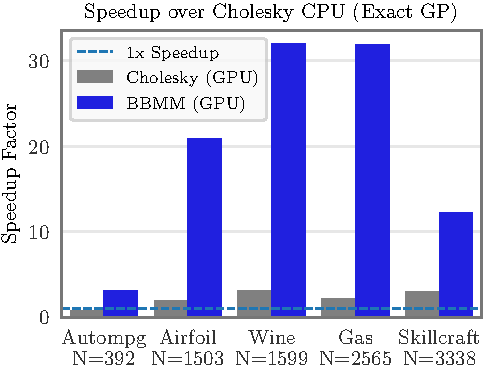
\includegraphics[width=0.45\textwidth]{figures/bbmm_speedup_exact_gp.pdf}
  \quad
  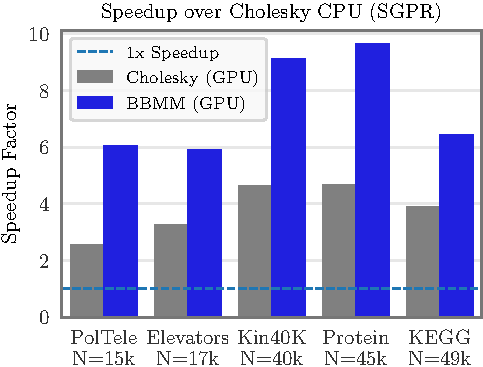
\includegraphics[width=0.45\textwidth]{figures/bbmm_speedup_sgpr.pdf}
  \vspace{1em}

  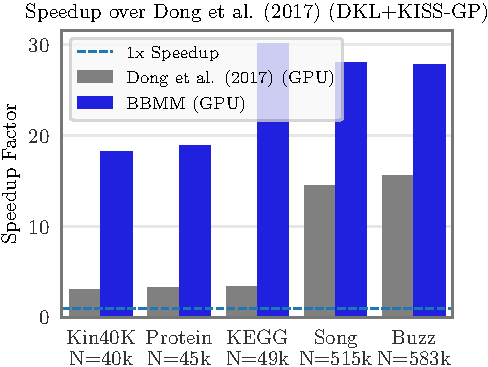
\includegraphics[width=0.45\textwidth]{figures/bbmm_speedup_dkl+kiss-gp.pdf}
  \caption[Speedup of GPU-accelerated GP training.]{
    Speedup of GPU-accelerated GP training.
    BBMM is in blue; competing GPU methods are in gray.
    {\bf Left:} Exact GP speedup over CPU Cholesky-based training.
    {\bf Middle:} SGPR \cite{titsias2009variational,hensman2013gaussian} speedup over CPU Cholesky-based training.
    {\bf Right:} KISS-GP+DKL \cite{wilson2015kernel,wilson2016deep} speedup over CPU training of \citet{dong2017scalable}.
    \label{fig:timing_results}
  }
\end{figure}
%
\begin{figure}[t]
  \centering
  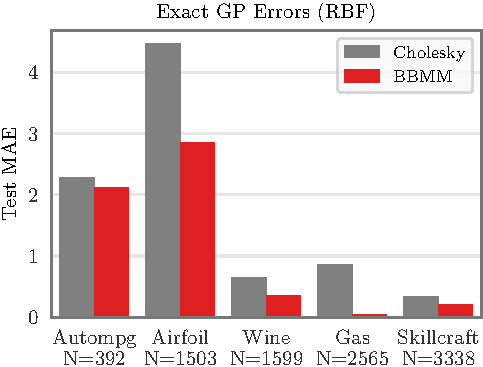
\includegraphics[width=0.45\textwidth]{figures/bbmm_error_exact_gp_RBF.pdf}
  \quad
  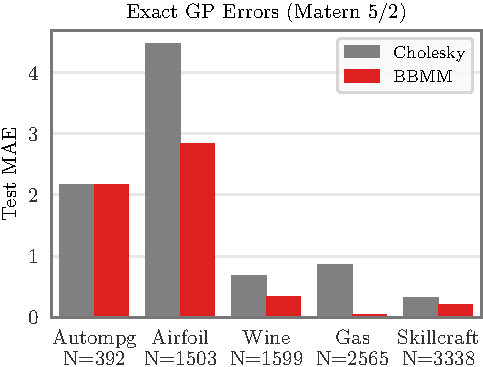
\includegraphics[width=0.45\textwidth]{figures/bbmm_error_exact_gp_Matern.pdf}
  \vspace{1em}

  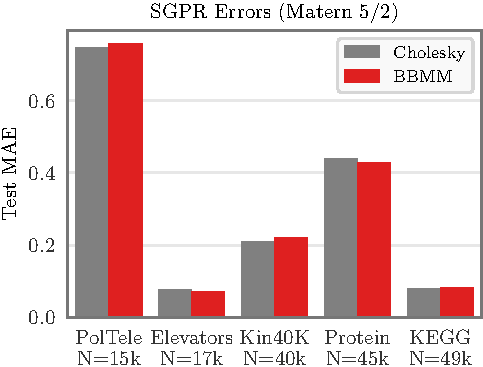
\includegraphics[width=0.45\textwidth]{figures/bbmm_error_sgpr_Matern.pdf}
  \caption[Predictive error comparison of mBCG versus Cholesky.]{
		Predictive error comparison of mBCG versus Cholesky (mean average error).
		The left two plots compare errors of Exact GPs with RBF and Mat\'ern-5/2 kernels,
		and the final plot compares error of SGPR models with a Mat\'ern-5/2 kernel.
	}
  \label{fig:bbmm_error_results}
\end{figure}

\paragraph{Speed comparison.}
\cref{fig:timing_results} shows the speedup obtained by GPU-accelerated BBMM over CPU-based training methods (Cholesky for Exact/SGPR, \citet{dong2017scalable} for KISS-GP).
BBMM is up to \emph{32 times faster} than Exact/KISS-GP CPU training, and up to 10 times faster than SGPR CPU training.
The largest speedups occur on the biggest datasets, since smaller datasets experience larger GPU overhead.
Notably, BBMM achieves a much larger speedup than GPU accelerated Cholesky methods (Exact, SGPR), which only achieve a roughly $4\times$ speedup.
This result underscores the fact that Cholesky methods are not as well suited for GPU acceleration.
For KISS-GP models, BBMM performs better than the GPU-accelerated method of \citet{dong2017scalable}.
This speedup is because BBMM is able to calculate all inference terms in parallel, while \citet{dong2017scalable} computes the terms in series.

\begin{figure}[t!]
  \begin{center}
    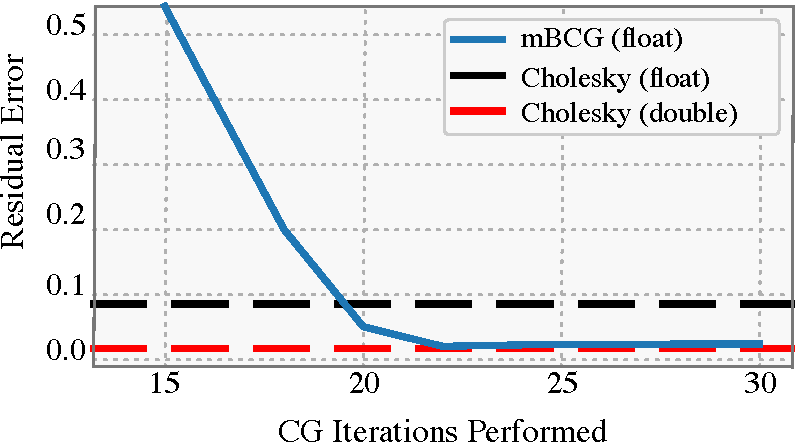
\includegraphics[width=0.50\textwidth]{figures/cg_error}
  \end{center}
  \caption{Solve error of mBCG versus Cholesky. \label{fig:cg_error}}
\end{figure}

\paragraph{Predictive error comparison.}
Computing predictive means requires the solve $\trainK^{-1} \by$.
Therefore, the PCG algorithm can be used to compute this term with preconditioning and GPU acceleration.
In \cref{fig:bbmm_error_results} we compare the mean average error (MAE) of BBMM models versus Cholesky models.
We demonstrate results using both the RBF kernel and a Mat\'ern-5/2 kernel.
Across all datasets, our method is at least as accurate in terms of final test MAE.
On a few datasets (e.g. Gas, Airfoil, and Wine with Exact GPs) BBMM even improves final test error.
The Cholesky decomposition is known to have numerical issues resulting from extremely small eigenvalues.
For example, Cholesky methods frequently add noise (or ``jitter'') to the diagonal of the kernel matrix for numerical stability.
It is possible to reduce the numerical instabilities with double precision (see \cref{fig:cg_error}); however, this requires an increased amount of computation.
BBMM on the other hand avoids adding this noise, without requiring double precision.

\begin{figure}[t]
  \centering
  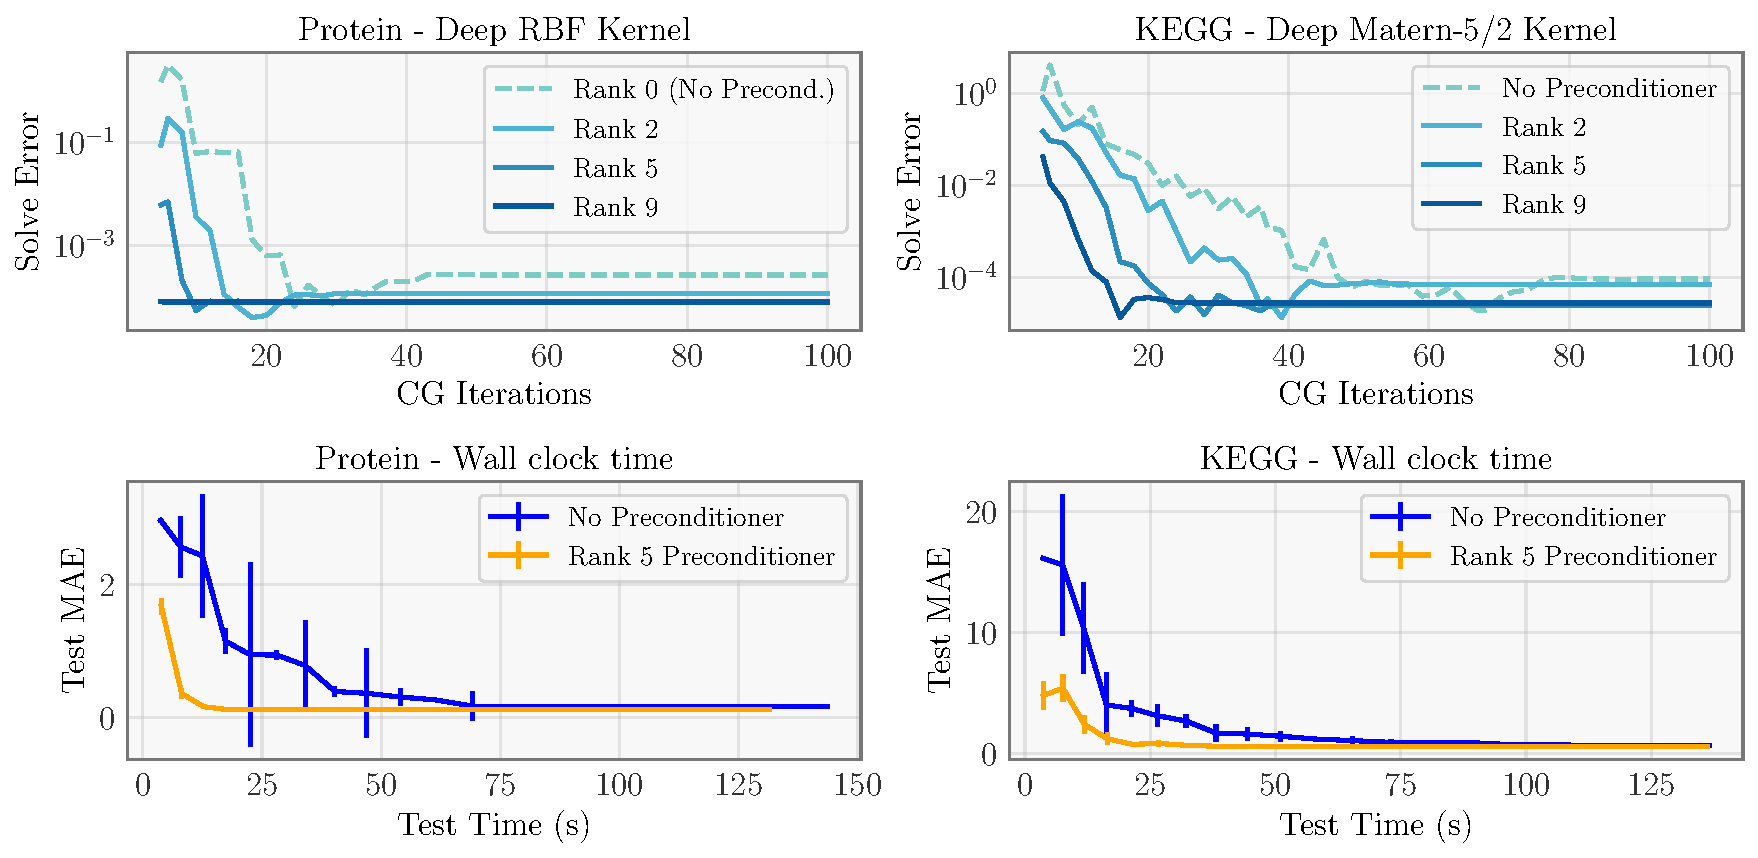
\includegraphics[width=\textwidth]{figures/precond_solves}
  \caption[Effect of partial pivoted Cholesky preconditioning on mBCG solve errors.]{
    Effect of partial pivoted Cholesky preconditioning.
		{\bf Top:} mBCG residual $\Vert \trainK \bc - \by \Vert / \Vert \by \Vert$ as a function of mBCG iterations.
    {\bf Bottom:} Test set mean average error (MAE) as a function of mBCG wall-clock time.
		Solves are computed using no preconditioner, rank $R=2$, $R=5$, and $R=9$ pivoted Cholesky preconditioners using deep RBF and deep Mat\'ern kernels.
		On the 2 datasets tested (Protein and KEGG), preconditioning accelerates convergence.
  }
  \label{fig:precond_results}
\end{figure}

\paragraph{Preconditioning.}
To demonstrate the effectiveness of preconditioning,
we train deep RBF and deep Mat\'ern-5/2 kernels on two datasets (Protein and KEGG) and evaluate the solve error of mBCG.
We measure the relative residual $\Vert \trainK\bc - \by \Vert / \Vert \by \Vert$ as a function of the number of mBCG iterations performed.
We compare using no preconditioner, as well as rank $R=2$, $R=5$, and $R=9$ partial pivoted Cholesky preconditioners.
The results are in the top of \cref{fig:precond_results}.
As expected based on our theoretical intuitions, increasing the rank of the preconditioner substantially reduces the number of mBCG iterations required to achieve convergence.

In \cref{fig:precond_results} (bottom), we confirm that these more accurate solves indeed result in faster training.
We plot the test MAE of preconditioned/non-preconditioned mBCG as a function of wall-time.\footnote{
  Wall-clock time is varied by changing the number of CG iterations.
}
We observe that a rank-5 preconditioner is indeed sufficient---the solves converge up to 5 times faster than without preconditioning.
Consequentially, we recommend always using the partial pivoted Cholesky preconditioner with BBMM.
It has virtually no wall-clock overhead and rapidly accelerates convergence.

%!TEX root=main_arxiv.tex
\section{Discussion}
In this chapter, we have presented a novel algorithm for Gaussian process training (BBMM) based on blackbox matrix-matrix multiplication routines with kernel matrices.
%We have implemented this framework and several state-of-the-art GP models in the {\href{https://gpytorch.ai}{GPyTorch}} package.
Below we discuss our findings and discuss extensions of BBMM that will be explored in future chapters.

\paragraph{Avoiding the Cholesky decomposition.}
An important takeaway of this chapter is that it is beneficial to avoid the Cholesky decomposition for GP training, even when no structured approximations are made.
We will explore the exact GP setting in more detail in \cref{chapter:largeexact} and further demonstrate the computational benefits of BBMM.

The Cholesky decomposition performs a large amount of computation to get a linear solve when fast iterative methods suffice.
Ultimately, the Cholesky decomposition of a full matrix takes $\bigo{N^3}$ time while CG takes $\bigo{N^2}$ time.
Indeed, as shown in \cref{fig:cg_error}, CG may even provide \emph{better} linear solves than the Cholesky decomposition.
%We liken this difference to the practical speed differences observed between second order methods like Newton's method and SGD in other settings.
%While we use a partial pivoted version of Cholesky for preconditioning, we only compute the first five rows of this decomposition.
%By terminating the algorithm very early, we avoid the computational bottleneck and many of the numerical instabilities.

\paragraph{Non-Gaussian likelihoods.}
When GP models are used with non-conjugate likelihoods (e.g. for classification or heavy-tailed noise models), we cannot compute the GP's marginal log likelihood (i.e. \cref{eqn:log_lik,eqn:log_lik_deriv} do not apply).
We must instead use variational approximations of the marginal log likelihood, which requires a different set of training and inference equations.
Importantly, it also requires computing the inverse square root of the kernel matrix times a vector ($\trainK^{- \frac 1 2} \bb$), which is not an output of the mBCG algorithm.
We will discuss how MVM techniques can be applied to this problem in \cref{chapter:ciq}.

\paragraph{Computing predictive distributions.}
The focus of this chapter has been optimizing the GP marginal log likelihood of \cref{eqn:log_lik,eqn:log_lik_deriv}.
The next chapter will focus on making predictions after a GP has been trained.
The equations for computing predictive distributions---\cref{eqn:predictive_mean,eqn:predictive_var}---require computing matrix solves.
%As suggested in this chapter, using MVM-based methods (e.g. preconditioned CG) for these solves will avoid the $\bigo{N^3}$ pitfalls of the Cholesky method.
In the next chapter, we will introduce a MVM based method that \emph{pre-computes and caches} most of the required CG computation.
This is especially beneficial when a GP is applied to large test sets.
With this pre-computation strategy, \cref{eqn:log_lik,eqn:log_lik_deriv} can both be reduced to $\bigo{N}$ computation, and $\bigo{1}$ computation when used in conjunction with KISS-GP.


%\input supplementary/modified_cg

%\input supplementary/pivoted_cholesky

%\input supplementary/convergence_theory

%\input supplementary/proofs

\chapter{Gaussian Process Predictions via Lanczos Variance Estimates}
\label{chapter:love}

%!TEX root=../main.tex
\section{Introduction}
Applying a Gaussian process model to previously-unseen test data returns a \emph{predictive distribution} rather than a point prediction.
Gaussian process predictive distribution are non-parametric and naturally adapt to the amount of training data.
As a result, these predictions tend to be well-calibrated---even for data points that lie far away from previously-seen training data \cite{rasmussen2006gaussian,wilson2014thesis}.
This property is crucial for applications where incorrect predictions could have catastrophic consequences, such as in medicine \cite{schulam2017if} or large-scale robotics \cite{deisenroth2015gaussian}.

This non-parametric formulation unfortunately comes with a computational downside.
Computing predictions with a GP requires performing linear solves with the $N \times N$ training covariance matrix (see \cref{eqn:predictive_mean,eqn:predictive_var}).
BBMM and recent advances in {inducing point methods} can be used to reduce some of these computational requirements.
Using a simple caching strategy (described in the next section), predictive means can be computed in $\bigo{N}$ time.
%For a test point $\bxtest$, the predictive mean is expressed as $\bk_{\bX\bxtest}^\top {\blue \ba}$, where $\blue \ba = \trainK^{-1} \by$ is a pre-computed solve dependent only on training data.
%After computing $\blue \ba$ in $\bigo{N^2}$ time using conjugate gradients, subsequent predictive means only require a $\bigo{N}$ inner product.
This computation can be reduced to $\bigo{1}$ when used in conjunction with Kernel Interpolation for Scalable Structured GP models (KISS-GP, see \cref{sec:kissgp}).

Unfortunately, predictive uncertainties remain a computational bottleneck, even with BBMM.
The predictive variance $\vartest{\bxtest}$ requires computing $\trainK^{-1} \bk_{\bX\bxtest}$ (see \cref{eqn:predictive_var}), which depends on the test point $\bxtest$ and therefore cannot be computed upfront.
%Consequentially the most expensive computations of \cref{eqn:predictive_var} cannot be easily pre-computed and cached.
%Additionally, drawing samples from the predictive distributions---a necessary operation in many applications---is similarly expensive.
%Existing fast approximations for these operations \cite{papandreou2011efficient,wilson2015thoughts,wang2017max} typically incur a significant amount of error.
Matching the complexity of predictive mean inference without sacrificing accuracy has remained an open problem.
The majority of this chapter is therefore dedicated to reducing the computational requirements of predictive variances.

We provide a matrix-vector multiplication (MVM) solution based on the tridiagonalization algorithm of \citet{lanczos1950iteration}.
We express the predictive covariance between $\bxtest$ and $\bxtestprime$ as
$\bk_{\bX\bxtest}^\top {\blue{\bC}} \: \bk_{\bX\bxtest}$,
where $\blue \bC \approx \trainK^{-1}$ is low-rank $N \times N$ approximation.
Using the Lanczos algorithm, we can efficiently form this low-rank decomposition using $J \ll N$ matrix-vector multiplications with $\trainK$.
After this one-time upfront computation, all variances can be computed in \emph{linear time} -- $\bigo{JN}$ -- per (co)-variance entry.
When used in conjunction with KISS-GP, this complexity can be further reduced to \emph{constant time}, and posterior samples can be drawn in \emph{linear time}.

We refer to this method as LanczOs Variance Estimates, or LOVE{} for short.
LOVE{} has the lowest asymptotic complexity for computing predictive (co)-variances with GPs.
We empirically validate LOVE{} on seven datasets and find that it consistently provides substantial speedups over existing methods \emph{without sacrificing accuracy}.
Variances and samples are accurate to within four decimals, and can be computed \emph{up to 18,000 times faster.}

\section{Motivation}
\label{sec:love_motivation}

\cref{eqn:predictive_mean} and \cref{eqn:predictive_var} describe how to compute predictive means and (co)-variances (restated below, assuming a prior mean of $\bzero$ for brevity):
%
\begin{align}
  \meantest{\bxtest}
  &= \bk_{\bX \bxtest}^\top {\color{blue} \trainK^{-1} \by}
  \label{eqn:predictive_mean_2}
  \\
  \covtest{\bxtest}{\bxtestprime}
  &= k(\bxtest, \bxtestprime) - \bk_{\bX\bxtest}^\top {\color{blue} \trainK^{-1}} \bk_{\bX\bxtestprime}.
  \label{eqn:predictive_covar_2}
\end{align}
%
The terms in {\color{blue} blue} represent terms that only depend on the training data.
If we are using a GP model to make a single prediction, then computing both of these terms requires a single call to conjugate gradients (${\color{blue} \trainK^{-1}} \bk^\top_{\bX\bxtest}$).
However, if we are making predictions on thousands of test points, these repeated CG calls may become prohibitively expensive, even when using the mBCG algorithm to parallelize the solves.
Since the expensive computations in \cref{eqn:predictive_mean_2,eqn:predictive_covar_2} primarily involve the training data terms, our goal is to \emph{pre-compute and cache} the most computationally intensive parts of these equations.
After this pre-computation, subsequent predictions ideally should be computationally cheap---i.e. $\bigo{N}$ or less.

\subsection{Computing Predictive Means}

Before discussing predictive (co)-variances, which will be the primary focus of this chapter, we will first discuss a pre-computation strategy for predictive means:
Since the ${\color{blue} \trainK^{-1} \by \triangleq \ba}$ term only depends on training data, it can be cached and re-used for all predictive means.
Each subsequent predictive mean is simply the inner product between the $\bk_{\bX \bxtest}$ vector and the pre-computed $\color{blue} \ba$ vector, which in general takes $\bigo{N}$ time.

This cost can be reduced even further for KISS-GP models, as discussed in \cref{sec:kissgp} and \citep{wilson2015thoughts}.
Recall that KISS-GP approximates the training and test covariances as:
%
\begin{align*}
  \tilde{\bk}_{\bX \bxtest} = \bW^\top_{\bX} \bK_{\bZ \bZ} \bw_{\bxtest},
  \quad
  \tilde{\bK}_{\bX \bX} = \bW^\top_{\bX} \bK_{\bZ \bZ} \bW_{\bX},
\end{align*}
%
where $\bK_{\bZ\bZ} \in \reals^{M \times M}$ is the Toeplitz inducing kernel matrix, $\bW_\bX \in \reals{M \times N}$ is the sparse interpolation for training points $X$, and $\bw_{\bxtest} \in \reals{M}$ is the sparse interpolation for $\bxtest$.
Plugging these approximations into \cref{eqn:predictive_mean_2} gives us
\[
  \meantest{\bxtest} = \bw_{\bxtest}^\top {\blue{\underbracket{\bK_{\bZ\bZ} \bW_{\bX}(\bW_{\bX}^{\top}\bK_{\bZ\bZ}\bW_{\bX} + \sigma_\text{obs}^{2} \bI)^{-1} \by}_{\ba'}}}.
\]
where again the blue terms only depend on training data.
After pre-computing the $\ba'$ vector, all subsequent means are the inner product between $\color{blue} \ba'$ and the \emph{$\bigo{1}$ sparse} $\bw_\bxtest$ vector.
These computations are $\bigo{1}$ because of this sparsity.

\subsection{Computing (Co)-Variances without Pre-computation}

The predictive (co)-variances are more challenging, as the only term in \cref{eqn:predictive_covar_2} that does not depend on test data is $\blue \trainK^{-1}$.
A common pre-computation is to form the Cholesky factorization $\blue \bL \bL^\top = \trainK$ ($\bigo{N^3}$ time, $\bigo{N^2}$ memory).
After factorization, all subsequent solves take $\bigo{N^2}$ time.
However, this cubic dependence on $N$ and quadratic memory may be infeasible for $N \geq 10,\!000$.

It is possible to obtain some computational savings when using inducing point methods.
For example, if we replace $\bk_{\bX \bxtest}$ and $\blue \trainK$ with their corresponding KISS-GP approximations in \cref{eqn:predictive_covar_2}, then we have:
%
\begin{align}
  \covtest{\bxtest}{\bxtestprime}
  &\approx
  k(\bxtest, \bxtestprime) -
  \bw_{\bxtest}^{\top} {\color{blue}\underbracket{{\bK_{\bZ\bZ} \bW_{\bX} \left( \bW^\top_{\bX} \bK_{\bZ\bZ} \bW_\bX + \sigma^2_\text{obs} \bI \right)^{-1} \bW^\top_{\bX} \bK_{\bZ \bZ}}}_{\blue \bC}} \bw_{\bxtestprime}.
  \label{eqn:pred_covar_approx}
\end{align}
%
$\blue \bC$, the braced portion of \cref{eqn:pred_covar_approx}, does not depend on the test points $\bxtest_{i}$, $\bxtest_{j}$ and therefore can be pre-computed during training.
The primary cost of this pre-computation is the $M$ solves with $\blue (\bW_\bX^\top {\bK}_{\bZ\bZ} \bW_\bX + \sigma_\text{obs}^2 \bI)$: one for each column vector in $\blue \bW^{\top}_{\bX} \bK_{\bZ\bZ}$, each of which takes $\bigo{N + M\log M}$ time with CG (see \cref{sec:kissgp} or \citet{wilson2015kernel}).
The total time for this pre-computation is therefore $\bigo{MN + M^2 \log M}$.
After pre-computation, \cref{eqn:pred_covar_approx} becomes
%
\begin{align}
  \covtest{\bxtest}{\bxtestprime} &\approx k_{\bxtest \bxtestprime} - \bw_{\bxtest}^\top \: {\blue \bC} \: \bw_{\bxtestprime}
    \label{eqn:pred_covar_ski_naive}
\end{align}
As $\bw_{\bxtest}$ contains only four nonzero elements, the inner product of $\bw^{*}_{i}$ with $\bC$ takes $\bigo{M}$ time.
Thus predictive covariances with \cref{eqn:pred_covar_ski_naive} are $\bigo{M}$ after pre-computation.

Although this technique offers computational savings over the Cholesky method, the quadratic dependence on $M$ in the pre-computation phase is a computational bottleneck.
In contrast, all other operations with KISS-GP require at most linear storage and near-linear time.
Indeed, one of the hallmarks of KISS-GP is the ability to use a very large number of inducing points $M = \Theta(N)$ so that kernel computations are nearly exact.


\section{LanczOs Variance Estimates (LOVE)}
\label{sec:love_method}

\input algorithms/love

We propose to overcome these limitations through an altered pre-computation step.
In particular, we can approximate $\blue \trainK$ in \cref{eqn:predictive_covar_2} as a low rank matrix.
Letting $\blue \bR$ be a $J \times N$ matrices such that $\blue \bR^\top \blue{\bR'} \approx \blue \trainK^{-1}$, we rewrite \cref{eqn:predictive_covar_2} as:
%
\begin{align}
  \covtest{\bxtest}{\bxtestprime}
  &= k(\bxtest, \bxtestprime) - ({\color{blue} \bR} \bk_{\bX\bxtest})^\top ({\color{blue} \bR} \bk_{\bX\bxtestprime}) + \sigma^2_\text{obs}
  \label{eqn:predictive_covar_2_fast}
\end{align}
%
Variance computations with \cref{eqn:predictive_covar_2_fast} take $\bigo{JN}$ time.

\paragraph{An MVM-based low-rank approximation with Lanczos.}
There are many possible ways to form a low-rank approximation of $\blue \trainK^{-1}$.
Our proposed method will make use of the Lanczos algorithm from \cref{sec:lanczos}, which will generate the low-rank approximation through matrix-vector multiplication (MVMs).
This makes it possible to easily transfer this approximation to specialty GP models (e.g. scalable models, multitask models, etc.) and the computation will effectively utilize GPU acceleration.
Moreover, as we will demonstrate in \cref{sec:love_results}, the Lanczos low-rank approximation rapidly converges to the true inverse.

Recall from \cref{sec:lanczos} that $J$ iterations of Lanczos tridiagonalization approximates matrix solves:
\[
  {\color{blue} \trainK^{-1}} \bb \approx {\color{blue} \bQ \bT^{-1} \bQ^{\top}} \bb,
\]
where the orthonormal matrix ${\color{blue} \bQ} \in \reals^{N \times J}$ and tridiagonal matrix ${\color{blue} \bT} \in \reals^{J \times J}$ are computed with respect to probe vector $\bb$.
As argued by \citet{parlett1980new}, \citet{saad1987lanczos}, and \citet{schneider2001krylov}, the $\blue \bQ$ and $\blue \bT$ matrices can be used to approximate subsequent solves
${\color{blue} \trainK^{-1}} \bb' \approx {\color{blue} \bQ \bT^{-1}} \bQ^\top \bb'$.
We exploit this fact and use $\blue \bQ \bT^{-1} \bQ^\top$ to be a general-purpose approximation to $\blue \trainK^{-1}$.
When $J \ll N$ (e.g. $J \approx 100$), then this will be a low-rank approximation.

To compute the $\bR$ matrix in \cref{eqn:predictive_covar_2_fast}, we simply run $J$ iterations of Lanczos:
\begin{align*}
  {\color{blue} \trainK^{-1}} &\approx \overbracket{\color{blue} \bQ \bT^{-1} \bQ^\top}^{\text{apply Lanczos}}
  \\
  &=
  \underbracket{ \left( {\color{blue} \bQ \bL_\bT^{-\top}} \right)}_{\color{blue} \bR^\top}
  \underbracket{ \left( {\color{blue} \bL_\bT^{-1} \bQ^\top} \right)}_{\color{blue} \bR}
\end{align*}
%
where $\blue \bL_\bT$ is the Cholesky factor of $\blue \bT$.
Applying Lanczos to $\blue \trainK$ requires $J$ MVMs for a total of $\bigo{J \mvm(\trainK)}$ time ($\mvm(\trainK)$ is the complexity of one MVM with $\blue \trainK$, which is nominally $\bigo{N^2}$).
Computing and applying the Cholesky factor $\blue \bL_\bT$ is $\bigo{J}$ time due to the tridiagonal structure of $\blue \bT$.

In total, the entire pre-computation phase takes $\bigo{J N^2}$ time for standard GPs.
This is the same amount of time of a single marginal likelihood computation using BBMM.
After pre-computation, each covariance takes $\bigo{JN}$ time.
We refer to this fast covariance approximation algorithm as {\bf LanczOs Variance Estimates}, or {\bf LOVE} for short.
It is summarized in \cref{alg:love} and \cref{tab:running_times}.

$J$, the size of the low-rank approximation, depends on the conditioning of $\blue \trainK$ and not its size.
Empirically find that $J\leq100$ is sufficient for most matrices for $N \leq 20,\!000$, and therefore $J$ can be considered to be constant.



\begin{table*}[t!]
  \caption[Asymptotic complexities of predictive (co)variances with LOVE verses other methods.]{
    Asymptotic complexities of predictive (co)variances ($N$ training points, $M$ inducing points, $J$ Lanczos/CG iterations).
    \label{tab:running_times}
  }
  \vspace{0.5ex}
  \centering
  \resizebox{\textwidth}{!}{%
    \begin{tabular}{ |c||c|c||c||c| }
  \hline
  \multirow{2}*{\bf Method} & \multicolumn{2}{c||}{\bf Pre-computation}  & {\bf Computing variances} & {\bf Drawing $s$ samples} \\
                            & \multicolumn{1}{c}{(time)} & (storage) & (time) & (time) \\
  \hhline{|=#=|=|=#=|}
  Standard GP
  & $\bigo{n^3}$
  & $\bigo{n^2}$
  & $\bigo{n^2}$
  & $\bigo{t n^2 + t^2 (n + s) + t^3}$
  \\
  SGPR
  & $\bigo{nm^2}$
  & $\bigo{m^2}$
  & $\bigo{m^2}$
  & $\bigo{t m^2 + t^2 (m + s) + t^3}$
  \\
  KISS-GP
  & --
  & --
  & $\bigo{k (n \! + \! m \log m)}$
  & $\bigo{k t (n \! + \! m \log m) \! + \! t^2 (m + s)  \! + \! t^3}$
  \\ \hline
  {\color{\ourmethodcolor} KISS-GP (w/ LOVE{})}
  & {\color{\ourmethodcolor}$\bigo{k (n \! + \! m \log m)}$}
  & {\color{\ourmethodcolor}$\bigo{km}$}
  & {\color{\ourmethodcolor}$\bigo{k}$}
  & {\color{\ourmethodcolor} $\bigo{k s (t + m)}$} \\
  \hline
\end{tabular}

  }
  \vspace{-2ex}
\end{table*}

\begin{table*}[t!]
  \caption[Asymptotic complexities of posterior sampling with LOVE + KISS-GP verses other methods.]{
    Asymptotic complexities of posterior sampling
		($N$ training points, $M$ inducing points, $J$ Lanczos/CG iterations, $S$ samples, $T$ test points).
    \label{tab:running_times_sampling}
  }
  \vspace{0.5ex}
  \centering
  \resizebox{\textwidth}{!}{%
    \begin{tabular}{ |c||c|c||c| }
  \hline
  \multirow{2}*{\bf Method} & \multicolumn{2}{c||}{\bf Pre-computation}  & {\bf Drawing $S$ samples} \\
                            & \multicolumn{1}{c}{(time)} & (storage) & (time) \\
  \hhline{|=#=|=|=|}
  Standard GP
  & --
  & --
  & $\bigo{T N^2 + T^2 (N + S) + T^3}$
  \\
  SGPR
  & --
  & --
  & $\bigo{T M^2 + T^2 (M + S) + T^3}$
  \\
  KISS-GP
  & --
  & --
  & $\bigo{J T (N  + M \log M) + T^2 (M + S) + T^3}$
  \\ \hline
  {\color{\ourmethodcolor} KISS-GP (w/ LOVE{})}
  & {\color{\ourmethodcolor}$\bigo{J (N + M \log M)}$}
  & {\color{\ourmethodcolor}$\bigo{JM}$}
  & {\color{\ourmethodcolor} $\bigo{J S (T + M)}$}
  \\ \hline
\end{tabular}

  }
  \vspace{-2ex}
\end{table*}


\subsection{Programmability.}

Because LOVE is an MVM-based algorithm, it affords the same modularity as BBMM.
When LOVE is used in conjunction with scalable GP approximations/multitask models, we can take advantage of fast kernel MVMs for a $o(N^2)$ asymptotic complexity.
In GPyTorch we use the {\tt LazyTensor} construct from \cref{sec:programmability} to adapt LOVE to specialty models.
The same {\tt \_matmul} function we use for mBCG can also be used in conjunction with LOVE for fast predictive (co)-variances.





\section{LOVE with KISS-GP}
\label{sec:love_method_kissgp}

\input algorithms/love_kissgp

As with BBMM, LOVE solely relies on matrix-vector multiplication and makes no assumption about the structure of $\blue \trainK$.
Therefore, \cref{alg:love} can be applied out-of-the-box to any specialty GP model including scalable approximations.
In this section, we demonstrate that LOVE is an especially compelling algorithm for the scalable KISS-GP framework.
With a few modifications to \cref{alg:love}, KISS-GP + LOVE can achieve \emph{constant-time covariance approximations} and \emph{linear time posterior samples}.

\subsection{Constant-Time (Co)-Variances with KISS-GP + LOVE}
The KISS-GP approximation $\color{blue} \bW_\bX^\top \bK_{\bZ \bZ} \bW_\bX$ allows us to make additional pre-computations to further reduce test-time complexity.
In particular,
%
\begin{align}
  \covtest{\bxtest}{\bxtestprime}
  &\approx k(\bxtest, \bxtestprime) - \bk_{\bX \bxtest}^\top {\color{blue} \bR^\top \bR} \bk_{\bX \bxtestprime} + \sigma^2_\text{obs}
  \nonumber
  \\
  &\approx k(\bxtest, \bxtestprime) - \left( \bw^\top_{\bxtest} \right. \underbracket{\left. {\color{blue} \bK_{\bZ\bZ} \bW_\bX} \right) {\color{blue} \bR^\top}}_{\color{blue} \widetilde \bR^\top}
  \underbracket{{\color{blue} \bR} \left( {\color{blue} \bW_\bX^\top \bK_{\bZ\bZ}} \right.}_{\color{blue} \bR} \left. \bw_{\bxtestprime} \right) + \sigma^2_\text{obs}
  \nonumber
  \\
  &\approx k(\bxtest, \bxtestprime) -
  \left( {\color{blue} \widetilde \bR} \bw^\top_{\bxtest} \right)^\top
  \left( {\color{blue} \widetilde \bR} \bw^\top_{\bxtestprime} \right) + \sigma^2_\text{obs}
  \label{eqn:pred_covar_ski_fast}
\end{align}
%
The matrix $\color{blue} \widetilde \bR = \bR \bK_{\bZ\bZ} \bW_\bX$ is a $J \times M$ matrix.
Variance computations with \cref{eqn:pred_covar_ski_fast} take $\bigo{J}$ time due to the sparsity of $\bw_{\bxtest}$ and $\bw_{\bxtestprime}$.
Choosing $J \approx 100$, which is sufficient for the conditioning of most matrices, KISS-GP covariance computations with \cref{eqn:pred_covar_ski_fast} take \emph{constant time}.

Moreover, this additional precomputation step takes negligible time.
The complexity of computing $\color{blue} \bR$ is $\bigo{J(N + M \log M)}$, as Lanczos requires $J$ MVMs with $\color{blue} \trainK$ and KISS-GP affords $\bigo{N + M \log M}$ MVMs.
Forming $\color{blue} \widetilde \bR$ requires multiplying the $J \! \times \! N$ $\color{blue} \bR$ matrix by $\color{blue} \bK_{\bZ\bZ}$ and $\color{blue} \bW_\bX$, which also takes $\bigo{J(N + M \log M)}$ time.
Therefore, the modified KISS-GP + LOVE precomputation is \emph{near-linear time}.
It is summarized in \cref{alg:love_kissgp} and \cref{tab:running_times}.

In addition to these fast predictive (co)-variances, LOVE + KISS-GP offers two additional speedups that are specific to KISS-GP models.




\subsection{Predictive Distribution Sampling with LOVE{} + KISS-GP}
\label{sec:sampling_method}

When used in conjunction with KISS-GP, LOVE{} can also be used to compute samples from the predictive covariance matrix.
This is a vary common operation: in Bayesian optimization, several popular acquisition functions---such as predictive entropy search \cite{hernandez2014predictive}, max-value entropy search \cite{wang2017max}, and knowledge gradient \cite{frazier2009knowledge}---require posterior sampling.

Let $\bXtest = [ \bxtest_1, \ldots, \bxtest_T ]$ be a test set of $T$ points.
To draw samples from $p( \ytest_1, \ldots, \ytest_T  \! \mid \! \dset)$---the predictive function evaluated on $\bxtest_1, \ldots, \bxtest_t$,
the cross-covariance terms (i.e. $\covtest{\bxtest_i}{\bxtest_j}$) are necessary in addition to the variance terms ($\vartest{\bxtest_i}$).
We sample $p( \bfn(\bxtest_1), \ldots, \bfn(\bxtest_T) \! \mid \! \dset)$ through the reparameterization trick \cite{kingma2014auto,rezende2014stochastic}:
%
\[
  \bmeantest = \begin{bmatrix} \meantest{\bxtest_1} \\ \vdots \\ \meantest{\bxtest_1} \end{bmatrix},
  \quad
  \Covtest = \begin{bmatrix}
    \covtest{\bxtest_1}{\bxtest_1} & \cdots & \covtest{\bxtest_1}{\bxtest_T} \\
    & \ddots & \\
    \covtest{\bxtest_T}{\bxtest_1} & \cdots & \covtest{\bxtest_T}{\bxtest_T} \\
  \end{bmatrix} - \sigma^2 \bI,
\]
\begin{equation}
  \bmeantest + \bS \bepsilon \sim p( \bfn(\bxtest_1), \ldots, \bfn(\bxtest_T) \! \mid \! \dset)
  \label{eqn:sample}
\end{equation}
%
where $\bepsilon \sim \normaldist{\bzero}{\bI}$ and $\bS \in \reals^{T \times T}$ is some matrix such that $\bS \bS^\top = \Covtest$.
Typically $\bS \bS^\top$ is taken to be the Cholesky decomposition of the predictive covariance matrix.
Computing this decomposition incurs a $\bigo{T^3}$ cost on top of the $\bigo{T^2}$ covariance evaluations.
This may be costly, even with constant-time covariance computations.

\paragraph{A Fast KISS-GP Sampling Matrix.}
We use LOVE{} and KISS-GP to rewrite \cref{eqn:pred_covar_ski_fast} as
%
\begin{align}
  \Covtest
  &\approx
  \bK_{\bXtest, \bXtest} - \overbracket{
    \bW^\top_{\bXtest} \left( {\color{blue} \widetilde \bR^\top \widetilde \bR} \right) \bW_{\bXtest}
  }^\text{LOVE + KISS-GP approximation}
  \nonumber
  \\
  &\approx \overbracket{
    \bW^\top_{\bXtest} {\color{blue} \bK_{\bZ\bZ} } \bW_{\bXtest}
  }^\text{KISS-GP approximation}
    \bW^\top_{\bXtest} \left( {\color{blue} \widetilde \bR^\top \widetilde \bR} \right) \bW_{\bXtest}
  \nonumber
  \\
  &= \bW^\top_{\bXtest} \left( {\color{blue} \bK_{\bZ\bZ} - \widetilde \bR^\top \widetilde \bR } \right) \bW_{\bXtest}
  \label{eqn:pred_covar_ski_interp_form12}
\end{align}
%
where $\bW_{\bXtest} = [\bw_{\bxtest_1}, \ldots, \bw_{\bxtest_T}]$ is the interpolation matrix for test points.
We have reduced the full covariance matrix to a test-independent term ($\blue{ \bK_{\bZ\bZ} - \widetilde \bR^\top \widetilde \bR }$) that can be pre-computed.
We apply the Lanczos algorithm on this term during pre-computation to obtain a rank-$J$ approximation:
%
\begin{align}
  { \color{blue} \bK_{\bZ\bZ} -  \widetilde \bR^\top \widetilde \bR' }
  \approx
  { \color{blue} \bQ' \bT' \bQ^{\prime\top} },
  \label{eqn:lancapprox}
\end{align}
%
where again $\bQ \in \reals^{M \times J}$ is orthonormal and $\bT \in \reals^{J \times J}$ is tridiagonal.
This Lanczos decomposition $\blue \bQ' \bT' \bQ^{\prime\top}$ requires $J$ matrix vector multiplies with $\blue{ \bK_{\bZ\bZ} - \widetilde \bR^{\top} \widetilde \bR }$, each of which requires $\bigo{M \log M}$ time.
Substituting \cref{eqn:lancapprox} into \cref{eqn:pred_covar_ski_interp_form12}, we get:
%
\begin{align}
  \Covtest
  &\approx \bW^\top_{\bXtest} \left( {\color{blue} \bQ' \bT' \bQ^{\prime\top} } \right) \bW_{\bXtest}
  \nonumber
  \\
  &= \bW^\top_{\bXtest} \left( {\color{blue} \bQ' \bL_{\bT'} } \right)
  \left( {\color{blue} \bL_{\bT^{\prime\top}} \bQ^{\prime\top} } \right) \bW_{\bXtest}
  \label{eqn:sampling_pre_cholesky}
\end{align}
where ${\color{blue} \bL_{\bT'} }$ is the Cholesky factor of $\blue \bT'$ (a $\bigo{J}$ operation due to the tridiagonal structure).
Setting $\blue{ \bS = \bQ' \bL_{\bT} }$, we see that $\Covtest = (\bW_{\bXtest}^\top {\blue \bS}) (\bW_{\bXtest}^\top {\blue \bS})^{\top}$.
${\blue S} \in \reals^{M \times J}$ can be pre-computed and cached since it does not depend on test data.
In total, this pre-computation takes $\bigo{J M \log M + M J^2}$ time in addition to what is required for fast variances.
To sample from the predictive distribution, we need to evaluate \cref{eqn:sample}, which involves multiplying $\bW^\top_{\bXtest} {\blue \bS} \bepsilon$.
Multiplying $\bepsilon$ by $\bS$ requires $\bigo{MJ}$ time, and finally multiplying by $\bW^{\top}_{\bXtest}$ takes $\bigo{TJ}$ time.
Therefore, drawing $S$ samples (corresponding to $S$ different values of $\bepsilon$) takes $\bigo{SJ(T + M)}$ time total during the testing phase (see \cref{tab:running_times_sampling})---a \emph{linear} dependence on $T$.



\subsection{Extension to Additive KISS-GP Kernel Compositions}
LOVE{} is applicable even when the KISS-GP approximation is used with an additive composition of kernels,
%
\begin{equation}
  \widetilde{k}(\bx, \bx') =
  \bw^{(1)\top}_{\bx} {\color{blue} \bK^{(1)}_{\bZ \bZ}} \bw^{(1)}_{\bx'} + \ldots + \bw^{(D)\top}_{\bx} {\color{blue} \bK^{(D)}_{\bZ \bZ}} \bw^{(D)}_{\bx'}.
  \notag
\end{equation}
Additive structure has recently been a focus in several Bayesian optimization settings, since the cumulative regret of additive models depends linearly on the number of dimensions
\cite{kandasamy2015high,wang2017batched,gardner2017discovering,wang2017max}.
Additionally, deep kernel learning GPs \citep{wilson2016deep,wilson2016stochastic} typically uses sums of one-dimensional kernel functions.
To apply LOVE{}, we note that additive composition can be re-written as
%
\begin{equation}
  \widetilde{k}(\bx, \bx') =
  \begin{bmatrix}
    \bw^{(1)}_{\bx} \\
    \vdots \\
    \bw^{(D)}_{\bx}
  \end{bmatrix}^\top
  \!
  {\color{blue}
  \begin{bmatrix}
    \bK^{(1)}_{\bZ \bZ} & \!\! \ldots \!\! & 0 \\
    \vdots & \!\! \ddots \!\! & \vdots \\
    0 & \!\! \ldots \!\! & \bK^{(D)}_{\bZ \bZ}
  \end{bmatrix}
  }
  \!
  \begin{bmatrix}
    \bw^{(1)}_{\bx} \\
    \vdots \\
    \bw^{(D)}_{\bx'}
  \end{bmatrix}.
  \label{eqn:multi_dimensional_kernel_block}
\end{equation}
%
The block matrices in \cref{eqn:multi_dimensional_kernel_block} are analogs of their 1-dimensional counterparts in \cref{eqn:ski}.
Therefore, we can directly apply \cref{alg:love_kissgp}, replacing $\blue \bW_\bX$, $\bw_\bxtest$, $\bw_\bxtestprime$, and $\blue \bK_{\bZ\bZ}$ with their block forms.
The block $\bw_\bxtest$, $\bw_\bxtestprime$ vectors are $\bigo{D}$-sparse, and therefore interpolation takes $\bigo{D}$ time.
MVMs with the block $\blue \bK_{\bZ\bZ}$ matrix take $\bigo{DM\log M}$ time by exploiting the block-diagonal structure.
With $D$ additive components, predictive variance computations cost only a factor $\bigo{D}$ more than their 1-dimensional counterparts.

%!TEX root=../main.tex
\section{Results}
\label{sec:love_results}

In this section we demonstrate the effectiveness and speed of KISS-GP + LOVE{}, both at computing predictive variances and also at posterior sampling.
Our goal is to show that 1) LOVE{} produces uncertainties and samples that are indistinguishable from the state-of-the-art, and 2) that LOVE{} offers substantial speed improvements.
All experiments in this section use LOVE in conjunction with KISS-GP models.
See \cref{chapter:largeexact} for results where LOVE is used with standard Gaussian processes.

In the following experiments, all LOVE{} low-rank approximations use $J=50$ Lanczos iterations and KISS-GP models use $M\!=\!10,\!000$ inducing points unless otherwise stated.
We optimize models with ADAM \cite{kingma2014adam} and a learning rate of $0.1$.
All timing experiments are performed on a GTX 1070 GPU.
Exact GPs, KISS-GP models, and LOVE are implemented in our GPyTorch software.
SGPR models are implemented in GPFlow \cite{matthews2017gpflow}.

\subsection{Predictive Variances}
\label{sec:results_variances}

We measure the accuracy and speed of LOVE + KISS-GP{} variances.
In all experiments, we compare against Exact GP ({\bf Exact}) variances (without LOVE) and standard KISS-GP variances ({\bf KISS-GP w/o LOVE}).
(Note that we do not compare predictive means, as LOVE{} only affects variance cmoputations.)
We report the scaled mean absolute error (SMAE)\footnote{
  Mean absolute error divided by the variance of $y$.
} \cite{rasmussen2006gaussian} of LOVE{} + KISS-GP variances compared against these baselines.
For each dataset, we optimize the hyperparameters of a KISS-GP model.
We then apply the same hyperparameters to each baseline model.

\begin{figure}[t!]
  \centering
  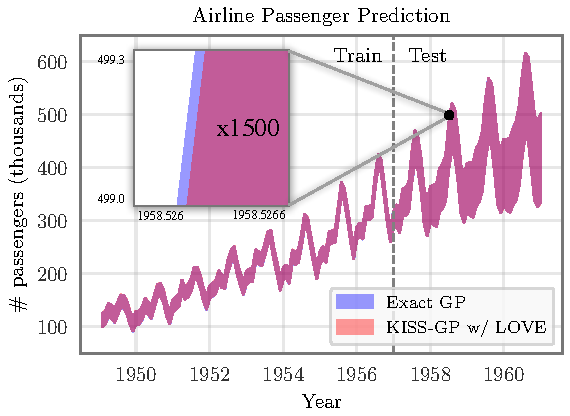
\includegraphics[width=0.65\columnwidth]{figures/airline_comparison.pdf}
  \caption[Comparison of LOVE predictive variances versus exact predictive variances on airline passenger extrapolation.]{
    Comparison of LOVE predictive variances versus exact predictive variances on airline passenger extrapolation.
    The LOVE{} variances are accurate within $10^{-4}$.
    \label{fig:airline_results}
  }
\end{figure}

\paragraph{One-dimensional example.}
We first demonstrate LOVE{} on a complex one-dimensional regression task.
The airline passenger dataset ({\bf Airline}) measures the average monthly number of passengers from 1949 to 1961 \cite{hyndman2005time}.
We aim to extrapolate the numbers for the final 4 years (48 measurements) given the first 8 years (96 measurements).
%These data exhibit short-term periodic trends as well as long-term growth trends.  Consequentially,
Accurate extrapolation on this dataset requires a kernel function capable of expressing various patterns, such as the spectral mixture (SM) kernel \cite{wilson2013gaussian}.
%Our goal is to evaluate if LOVE{} produces reliable predictive variances, even with complex kernel functions.

We compute the variances for Exact GP and KISS-GP + LOVE{} models with a $10$-mixture SM kernel.
In \cref{fig:airline_results}, we see that the LOVE + KISS-GP{} confidence intervals match the Exact GP's intervals extremely well.
The SMAE of LOVE{}'s predicted variances (compared against Exact GP variances) is $1.29 \times 10^{-4}$.
Although not shown in the plot, we confirm the reliability of these predictions by computing the log-likelihood of the test data.
We compare the LOVE + KISS-GP{} model to an Exact GP, a KISS-GP model without LOVE{}, and a sparse variational GP (SGPR) model with $M=1000$ inducing points.
All methods achieve nearly identical log-likelihoods, ranging from $-221$ to $-222$.


\begin{table}[t!]
  \caption[Speedup and accuracy of LOVE + KISS-GP{} for predictive variances.]{
    Speedup and accuracy of LOVE + KISS-GP{} for predictive variances (Deep RBF Kernels).
    Accuracy is measured by Scaled Mean Average Error.
    ($N$ is the number of data, $D$ is the dimensionality.)
    \label{tab:large_dataset_results}
  }
  \vspace{0.5ex}
  \centering
  \resizebox{\textwidth}{!}{%
    %!TEX root=../main.tex
\begin{tabular}{ |ccc||c|c||c|c| }
  \hline
  \multicolumn{3}{|c|}{\bf Dataset}
  & \multicolumn{4}{c|}{\thead{\bf Variance SMAE}}
  \\
  \cline{1-7}
  Name
  & {$N$}
  & {$D$}
  & {\thead{(vs KISS-GP w/o LOVE)}}
  & {\thead{(vs Exact GP)}}
  & {\thead{(from scratch)}}
  & {\thead{(after pre-comp.)}}
  \\
  \hhline{|===#=|=#=|=|}
  \thead{\bf Airfoil}
  & $1,\!503$
  & $6$
  & $1.30 \times 10^{-5}$
  & $7.01 \times 10^{-5}$
  & $4 \times$
  & $84 \times$
  %& $3 \times$
  %& $49 \times$
  %& $9 \times$
  %& $183 \times$
  \\

  \thead{\bf Skillcraft}
  & $3,\!338$
  & $19$
  & $2.00 \times 10^{-7}$
  & $2.86 \times 10^{-4}$
  & $25 \times$
  & $167 \times$
  %& $4 \times$
  %& $70 \times$
  %& $17 \times$
  %& $110 \times$
  \\

  \thead{\bf Parkinsons}
  & $5,\!875$
  & $20$
  & $8.80 \times 10^{-5}$
  & $5.18 \times 10^{-3}$
  & $46 \times$
  & $443 \times$
  %& $3 \times$
  %& $33 \times$
  %& $16 \times$
  %& $152 \times$
  \\

  \thead{\bf PoleTele}
  & $15,\!000$
  & $26$
  & $2.90 \times 10^{-5}$
  & $1.08 \times 10^{-3}$
  & $78 \times$
  & $1178 \times$
  %& $1.5 \times$
  %& $40 \times$
  %& $21 \times$
  %& $343 \times$
  \\

  \thead{\bf Elevators}
  & $16,\!599$
  & $18$
  & $1.20 \times 10^{-6}$
  & --
  & $64 \times$
  & $1017 \times$
  %& $2 \times$
  %& $31 \times$
  %& $20 \times$
  %& $316 \times$
  \\

  \thead{\bf Kin40k}
  & $40,\!000$
  & $8$
  & $3.90 \times 10^{-7}$
  & --
  & $31 \times$
  & $2065 \times$
  %& $8 \times$
  %& $81 \times$
  %& $12 \times$
  %& $798 \times$
  \\

  \thead{\bf Protein}
  & $45,\!730$
  & $9$
  & $5.30 \times 10^{-5}$
  & --
  & $44 \times$
  & $1151 \times$
  %& $10 \times$
  %& $109 \times$
  %& $20 \times$
  %& $520 \times$
  \\
  \hline
\end{tabular}

  }
  \vspace{1em}

  \resizebox{\textwidth}{!}{%
    %!TEX root=../main.tex
\begin{tabular}{ |ccc||c|c|c|c| }
  \hline
  \multicolumn{3}{|c||}{\bf Dataset}
  & \multicolumn{4}{c|}{\thead{\bf Speedup over SGPR}}
  \\
  \cline{1-7}
  \multirow{2}{*}{Name}
  & \multirow{2}{*}{$N$}
  & \multirow{2}{*}{$D$}
  & \thead{(from scratch)}
  & \thead{(after pre-comp.)}
  & \thead{(from scratch)}
  & \thead{(after pre-comp.)}
  \\
   &  &  & $M=100$ & $M=100$ & $M=1000$ & $M=1000$
  \\
  \hhline{|===#=|=|=|=|}
  \thead{\bf Airfoil}
  & $1,\!503$
  & $6$
  %& $1.30 \times 10^{-5}$
  %& $7.01 \times 10^{-5}$
  %& $4 \times$
  %& $84 \times$
  & $3 \times$
  & $49 \times$
  & $9 \times$
  & $183 \times$
  \\

  \thead{\bf Skillcraft}
  & $3,\!338$
  & $19$
  %& $2.00 \times 10^{-7}$
  %& $2.86 \times 10^{-4}$
  %& $25 \times$
  %& $167 \times$
  & $4 \times$
  & $70 \times$
  & $17 \times$
  & $110 \times$
  \\

  \thead{\bf Parkinsons}
  & $5,\!875$
  & $20$
  %& $8.80 \times 10^{-5}$
  %& $5.18 \times 10^{-3}$
  %& $46 \times$
  %& $443 \times$
  & $3 \times$
  & $33 \times$
  & $16 \times$
  & $152 \times$
  \\

  \thead{\bf PoleTele}
  & $15,\!000$
  & $26$
  %& $2.90 \times 10^{-5}$
  %& $1.08 \times 10^{-3}$
  %& $78 \times$
  %& $1178 \times$
  & $1.5 \times$
  & $40 \times$
  & $21 \times$
  & $343 \times$
  \\

  \thead{\bf Elevators}
  & $16,\!599$
  & $18$
  %& $1.20 \times 10^{-6}$
  %& --
  %& $64 \times$
  %& $1017 \times$
  & $2 \times$
  & $31 \times$
  & $20 \times$
  & $316 \times$
  \\

  \thead{\bf Kin40k}
  & $40,\!000$
  & $8$
  %& $3.90 \times 10^{-7}$
  %& --
  %& $31 \times$
  %& $2065 \times$
  & $8 \times$
  & $81 \times$
  & $12 \times$
  & $798 \times$
  \\

  \thead{\bf Protein}
  & $45,\!730$
  & $9$
  %& $5.30 \times 10^{-5}$
  %& --
  %& $44 \times$
  %& $1151 \times$
  & $10 \times$
  & $109 \times$
  & $20 \times$
  & $520 \times$
  \\
  \hline
\end{tabular}

  }
\end{table}

\paragraph{Large datasets.}
We measure the accuracy of LOVE{} variances on several large-scale regression benchmarks from the UCI repository \cite{asuncion2007uci}.
%We compute the variance for all test set data points.
Each of the models use deep RBF kernels (DKL) with the architectures described in \cite{wilson2016deep}.
%Deep RBF kernels are extremely flexible (with up to $10^5$ hyperparameters) and are well suited to model many types of functions.
In \cref{tab:large_dataset_results}, we report the SMAE of the LOVE + KISS-GP{} variances compared against the two baselines.
On all datasets, we find that LOVE{} matches KISS-GP w/o LOVE{} to at least $5$ decimal places.
Furthermore, LOVE + KISS-GP{} is able to approximate Exact variances with no more than than $10^{-3}$ error.
For any given test point, the maximum variance error is similarly small (e.g. $\leq \! 2.6\%$ on Skillcraft and $\leq \! 2.0\%$ on PoleTele).
Therefore, using LOVE{} to compute variances results in \emph{almost no loss in accuracy}.

\paragraph{Speedup.}
In \cref{tab:large_dataset_results} we compare the variance computation speed of a KISS-GP model with and without LOVE{} on the UCI datasets.
In addition, we compare against SGPR models (with non-deep RBF kernels), a competitive scalable GP approach.
On all datasets, we measure the time to compute variances {\bf from scratch}, which includes the cost of pre-computation.
In addition, we report the speed {\bf after pre-computing} any terms that aren't specific to test points.
We see in \cref{tab:large_dataset_results} that KISS-GP + LOVE{} yields a substantial speedup over KISS-GP without LOVE{}.
The speedup is between $4\times$ and $44\times$, even when accounting for LOVE{}'s precomputation.
At test time after pre-computation, LOVE{} is \emph{up to $2,\!000\times$ faster}.
Additionally, LOVE + KISS-GP{} is significantly faster than SGPR models.
For SGPR models with $M=100$ inducing points, the LOVE + KISS-GP{} model (with $M=10,\!000$ inducing points) is up to $10\times$ faster before pre-computation and $100\times$ faster after.
With $M=1000$ SGPR models, LOVE + KISS-GP{} is up to $20\times$/$500\times$ faster before/after precomputation.
The biggest improvements are obtained on the largest datasets since LOVE{}, unlike other methods, is independent of dataset size at test time.

\begin{figure}[t!]
  \centering
  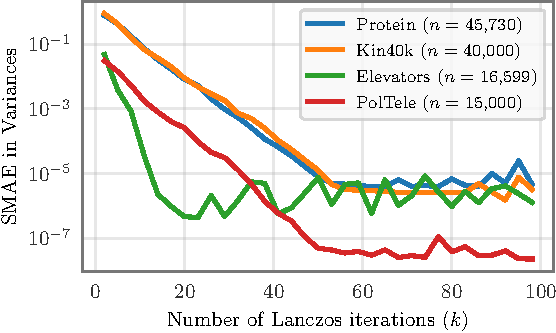
\includegraphics[width=0.65\columnwidth]{figures/lanczos_accuracy.pdf}
  \vspace{-2ex}
  \caption[LOVE variance error as a function of Lanczos iterations.]{
    LOVE variance error as a function of Lanczos iterations
    (KISS-GP model, $M=10,\!000$. Protein, Kin40k, PoleTele, and Elevators UCI datasets).
    \label{fig:lanczos_accuracy}
  }
  \vspace{-1ex}
\end{figure}

\paragraph{Accuracy vs. Lanczos iterations.}
In \cref{fig:lanczos_accuracy}, we measure the accuracy of LOVE{} as a function of the number of Lanczos iterations ($J$), which corresponds to the rank of the $\blue \widetilde \bR$ matrix in \cref{eqn:pred_covar_ski_fast}.
We train a KISS-GP model with a deep RBF kernel on the four largest datasets from \cref{tab:large_dataset_results}, measuring the SMAE of LOVE + KISS-GP's predictive variances.\footnote{
  As measured against the variances from KISS-GP w/o LOVE.
}
As seen in \cref{fig:lanczos_accuracy}, error decreases \emph{exponentially} with the number of Lanczos iterations, up until roughly $50$ iterations.
After roughly $50$ iterations, the error levels off, though this may be an artifact of floating-point precision (which may also cause small subsequent fluctuations).



\subsection{Sampling}

\begin{table}[t!]
  \caption[Accuracy and computation time of drawing samples from the posterior distribution.]{
    Accuracy and computation time of drawing samples from the posterior distribution.
    \label{tab:sampling_results}
  }
  \vspace{0.5ex}
  \centering
  \resizebox{\textwidth}{!}{%
    %!TEX root=../main.tex
\begin{tabular}{ |c||c|c|c|c|c| }
  \hline
  \multirow{4}{*}{\thead{\bf Dataset} }
  & \multicolumn{5}{c|}{\thead{\bf Sample Covariance Error} }

  \\
  \cline{2-6}


  & \thead{\bf Exact GP \\ \bf w/ Cholesky}
  & \thead{\bf Fourier \\ \bf Features}
  & \thead{\bf SGPR \\ ($M=100$)}
  & \thead{\bf SGPR \\ ($M=1000$)}
  & \thead{\bf LOVE \\ \bf + KISS-GP}
  %& \thead{\bf Fourier \\ \bf Features}
  %& \thead{\bf SGPR (m=100)}
  %& \thead{\bf SGPR (m=1000)}
  %& \thead{\bf KISS-GP \\ \bf w/ LOVE{} \\ (from scratch)}
  %& \thead{\bf KISS-GP \\ \bf w/ LOVE{} \\ (after pre-comp.)}
  \\
  \hhline{|=#=|=|=|=|=|}

  \thead{\bf PolTele}
  & $\mathbf{8.8 \times 10^{-4}}$
  & $1.8 \times 10^{-3}$
  & $4.9 \times 10^{-3}$
  & $2.7 \times 10^{-3}$
  & $\mathbf{7.5 \times 10^{-4}}$
  %& $22 \times$
  %& $24 \times$
  %& $3 \times$
  %& $21 \times$
  %& $\mathbf{881 \times}$
  \\

  \thead{\bf Elevators}
  & $\mathbf{2.6 \times 10^{-7}}$
  & $3.1 \times 10^{-4}$
  & $8.7 \times 10^{-6}$
  & $3.6 \times 10^{-6}$
  & $\mathbf{5.5 \times 10^{-7}}$
  %& $31 \times$
  %& $33 \times$
  %& $4 \times$
  %& $25 \times$
  %& $\mathbf{1062 \times}$
  \\
  \hline

  \thead{\bf BO (Eggholder)}
  & $\mathbf{7.7 \times 10^{-4}}$
  & $1.5 \times 10^{-3}$
  & $\mathbf{8.1 \times 10^{-4}}$
  & --
  & $\mathbf{8.0 \times 10^{-5}}$
  %& $16 \times$
  %& $8 \times$
  %& --
  %& $19 \times$
  %& $\mathbf{775 \times}$
  \\

  \thead{\bf BO (Styblinski-Tang)}
  & $\mathbf{5.4 \times 10^{-4}}$
  & $7.3 \times 10^{-3}$
  & $\mathbf{5.2 \times 10^{-4}}$
  & --
  & $\mathbf{5.2 \times 10^{-4}}$
  %& $11 \times$
  %& $8 \times$
  %& --
  %& $42 \times$
  %& $\mathbf{18,\!100 \times}$
  \\
  \hline

\end{tabular}

  }
  \vspace{1em}

  \resizebox{\textwidth}{!}{%
    %!TEX root=../main.tex
\begin{tabular}{ |c||c|c|c|c|c| }
  \hline
  \multirow{4}{*}{\thead{\bf Dataset} }
  & \multicolumn{5}{c|}{\thead{\bf Speedup over Exact GP w/ Cholesky} }

  \\
  \cline{2-6}


  %& \thead{\bf Exact GP \\ \bf w/ Cholesky}
  %& \thead{\bf Fourier \\ \bf Features}
  %& \thead{\bf SGPR (m=100)}
  %& \thead{\bf SGPR (m=1000)}
  %& \thead{\bf KISS-GP \\ \bf w/ LOVE}
  & \thead{\bf Fourier \\ \bf Features}
  & \thead{\bf SGPR \\ ($M=100$)}
  & \thead{\bf SGPR \\ ($M=1000$)}
  & \thead{\bf LOVE \\ \bf + KISS-GP{} \\ (from scratch)}
  & \thead{\bf LOVE \\ \bf + KISS-GP{} \\ (after pre-comp.)}
  \\
  \hhline{|=#=|=|=|=|=|}

  \thead{\bf PolTele}
  %& $\mathbf{8.8 \times 10^{-4}}$
  %& $1.8 \times 10^{-3}$
  %& $4.9 \times 10^{-3}$
  %& $2.7 \times 10^{-3}$
  %& $\mathbf{7.5 \times 10^{-4}}$
  & $22 \times$
  & $24 \times$
  & $3 \times$
  & $21 \times$
  & $\mathbf{881 \times}$
  \\

  \thead{\bf Elevators}
  %& $\mathbf{2.6 \times 10^{-7}}$
  %& $3.1 \times 10^{-4}$
  %& $8.7 \times 10^{-6}$
  %& $3.6 \times 10^{-6}$
  %& $\mathbf{5.5 \times 10^{-7}}$
  & $31 \times$
  & $33 \times$
  & $4 \times$
  & $25 \times$
  & $\mathbf{1062 \times}$
  \\
  \hline

  \thead{\bf BO (Eggholder)}
  %& $\mathbf{7.7 \times 10^{-4}}$
  %& $1.5 \times 10^{-3}$
  %& $\mathbf{8.1 \times 10^{-4}}$
  %& --
  %& $\mathbf{8.0 \times 10^{-5}}$
  & $16 \times$
  & $8 \times$
  & --
  & $19 \times$
  & $\mathbf{775 \times}$
  \\

  \thead{\bf BO (Styblinski-Tang)}
  %& $\mathbf{5.4 \times 10^{-4}}$
  %& $7.3 \times 10^{-3}$
  %& $\mathbf{5.2 \times 10^{-4}}$
  %& --
  %& $\mathbf{5.2 \times 10^{-4}}$
  & $11 \times$
  & $8 \times$
  & --
  & $42 \times$
  & $\mathbf{18,\!100 \times}$
  \\
  \hline

\end{tabular}

  }
\end{table}

We evaluate the quality of posterior samples drawn with LOVE + KISS-GP{} as described in \cref{sec:sampling_method}.
We compare against three baselines: sampling from an {\bf Exact GP} using the Cholesky decomposition, sampling from an {\bf SGPR} model with Cholesky, and sampling an exact GP with random {\bf Fourier features} \citep{rahimi2008random}.
%The LOVE + KISS-GP{} and SGPR models use the same architecture as described in the previous section.
For Fourier features, we use 5000 random features---the maximum number of features without exhausting available GPU memory.
The model hyperparameters are learned on an Exact GP and then shared across all baselines.
We use two UCI datasets (PolTele and Eleveators) datasets as well as two Bayesian optimization (BO) benchmark functions (Eggholder: 2 dimensional, and Styblinski-Tang: 10 dimensional).
For the BO functions, we evaluate the model after 100 queries of max value entropy search \cite{wang2017max}.
For Eggholder, we use a standard (non-deep) RBF kernel;  for Syblinski-Tang we use the additive kernel suggested by~\citet{kandasamy2015high}.\footnote{
  The Syblinski-Tang KISS-GP model uses the sum of 10 RBF kernels---one for each dimension---and $M=100$ inducing points.
}

\paragraph{Sampling accuracy.}
In \cref{tab:sampling_results} we evaluate the accuracy of the different sampling methods.
We draw $S\!=\!1000$ samples at $T\!=\!10,\!000$ test locations and compare the empirical covariance matrix with the true posterior covariance.
The reported numbers are element-wise mean absolute errors.
It is worth noting that all methods incur some sampling error---even when sampling with an Exact GP.
Nevertheless, Exact GPs, SGPR, and LOVE{} produce very accurate sample covariance matrices.
In particular, Exact GPs and LOVE{} achieve between 1 and 3 orders of magnitude less error than the random Fourier Feature method.

\paragraph{Speed.}
Though LOVE{}, Exact GPs, and SGPR have similar accuracies, LOVE{} is much faster.
Even when accounting for LOVE's pre-computation time (i.e. sampling ``from scratch''), LOVE{} is comparable to Fourier features and SGPR in terms of speed.
At test time (i.e. after pre-computation), LOVE{} is up to $18,\!000$ times faster than Exact.

\paragraph{Bayesian optimization.}
Many acquisition functions in Bayesian optimization rely on sampling from the GP posterior.
For example, max-value entropy search \cite{wang2017max} uses samples to estimate the function's maximum value $p(y_\text{max} \! \mid \! \dset)$.
%
\begin{figure}[t!]
  \centering
  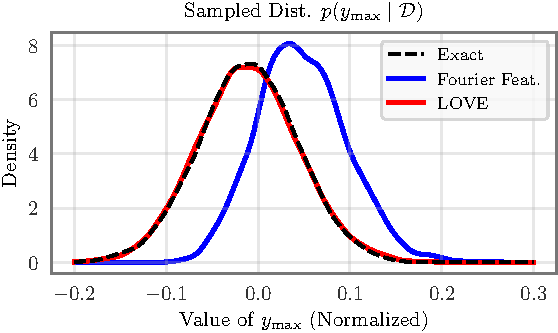
\includegraphics[width=0.65\columnwidth]{figures/love_sampling_comparison.pdf}
  \caption[Comparison of LOVE versus Random Fourier Features for Bayesian optimization via Max-Value Entropy Search.]{
    Comparison of LOVE versus Random Fourier Features for Bayesian optimization (BO) via Max-Value Entropy Search.
    Each line represents an approximation of the maximum value distribution $p(y_\text{max} \mid \dset)$ using different sampling methods (exact sampling, Random Fourier Features, and LOVE + KISS-GP).
    Samples drawn with LOVE+KISSGP closely match samples drawn using an Exact GP.
    (Dataset: (normalized) Eggholder function after 100 iterations of BO.)
    \label{fig:love_sampling_comparison}
  }
\end{figure}
%
In \cref{fig:love_sampling_comparison}, we visualize each method's sampled distribution of $p(y_\text{max} \! \mid \! \dset)$ for the Eggholder function.
We plot kernel density estimates of this distribution after $100$ BO iterations.\footnote{
  Using the max-value entropy search acquisition function \citep{wang2017max}.
}
Since the Exact GP sampling method uses the Cholesky decomposition, its sampled max-value distribution can be considered closest to ground truth.
The Fourier feature distribution differs significantly from the Exact GP distribution.
In contrast, LOVE{} very closely resembles Exact GPs, yet can be computed up to $700 \times$ faster (\cref{tab:sampling_results}).

%!TEX root=../main.tex
\section{Discussion}
\label{sec:love_discussion}

This chapter has introduced the LOVE algorithm for exact GPs and KISS-GP models.
Whereas the running times of previous methods depend on dataset size, LOVE{} + KISS-GP provides \emph{constant time} and near-exact predictive variances.
It is worth noting that LOVE is fully compatible with other inducing point techniques as well, as the algorithm is defined by a matrix-vector multiplication routine.
%Many inducing point methods make use of the subset of regressors (SOR) kernel approximation $\bK_{\bX\bX} \approx \bK_{\bX\bZ}\bK_{\bZ\bZ}^{-1}\bK_{\bZ\bX}$,
%optionally with a diagonal correction \cite{snelson2006sparse}, and focus on the problem of learning the inducing point locations \cite{quinonero2005unifying,titsias2009variational}.
%After $\bigo{M^{3}}$ work to Cholesky decompose $\bigo{\bK_{\bZ\bZ}}$, this approximate kernel affords $\bigo{N + M^{2}}$ MVMs.
For example, one could apply LOVE to SGPR using the efficient MVM described in \cref{sec:programmability}.
Since SGPR makes a rank $M \ll N$ approximation to the kernel, setting $J\!=\!M$ recovers the $\bigo{NM^{2}}$ precomputation time and $\bigo{M^2}$ prediction time of standard SGPR variances \cite{titsias2009variational}.

\paragraph{Ensuring Lanczos solves are accurate.}
Given a matrix $\blue \trainK$, the Lanczos decomposition $\blue \bQ \bT \bQ^\top$ is designed to approximate the solve ${\color{blue} \trainK^{-1}} \bb$, where $\bb$ is the first column of $\blue \bQ$.
As argued in \cref{sec:lanczos}, the $\blue \bQ$ and $\blue \bT$ matrices can usually be re-used to approximate the solves ${\color{blue} \widehat \bK_{\bX\bX}^{-1} (\bW_{\bX}^\top \bK_{\bZ\bZ})} \approx {\color{blue} \bQ \bT^{-1} \bQ^\top (\bW_{\bX}^\top \bK_{\bZ\bZ})}$.
This property of the Lanczos algorithm is why LOVE{} can compute fast predictive variances.
While this method usually produces accurate solves, the solves will not be accurate if some columns of $\blue (\bW^\top_{\bX} \bK_{\bZ\bZ})$ are (nearly) orthogonal to the columns of $\blue \bQ$.
Importantly, we can easily check the accuracy of the solves by measuring the residual norm:
%
\[
  \Vert {\blue \trainK} \underbracket{\left( {\color{blue} \bR \bR^\top} \right)}_{\blue \approx \trainK^{-1}} \bk_{\bX \bxtest} - \bk_{\bX \bxtest} \Vert_2.
\]
%
Note that this convergence check only requires an additional MVM with $\blue \trainK$.
If the residual is not sufficiently small for some vector $\bk_{\bX \bxtest}$, we can run conjugate gradients to refine the solve ${\blue \trainK^{-1}} \bk_{\bX \bxtest}$ using ${\color{blue} \bR \bR^\top} \bk_{\bX \bxtest}$ as an initial starting vector.
In practice, we find that these countermeasures are almost never necessary with LOVE{}---the Lanczos solves are almost always accurate.

\paragraph{Numerical stability of Lanczos.}
A practical concern for LOVE{} is round-off errors that may affect the Lanczos algorithm.
In particular it is common for the vectors of $\blue \bQ$ to lose orthogonality \cite{paige1970practical,simon1984lanczos,golub2012matrix}, resulting in an incorrect decomposition.
To correct for this, several methods such as full reorthogonalization and partial or selective reorthogonalization exist \citep[e.g.][]{golub2012matrix}.
In our implementation, we use full reorthogonalization when a loss of orthogonality is detected.
In practice, the cost of this correction is absorbed by the parallel performance of the GPU and does not impact the final running time.


\paragraph{Sampling without KISS-GP.}
LOVE in conjunction with KISS-GP makes it possible to efficiently draw samples from a GP posterior.
This has potential in many applications like Bayesian optimization and model-based reinforcement learning \citep[e.g.,][]{deisenroth2011pilco,hernandez2014predictive,wang2017max}, which typically rely on parametric approximations or finite basis approaches for approximate sampling.
However, it is worth noting that this sampling technique cannot be applied to exact GP models,
as the derivation of LOVE sampling requires an inducing point approximation to the prior test covariance $\bK_{\bXtest\bXtest}$ (see \cref{eqn:pred_covar_ski_interp_form12}).
In the next chapter we will address this limitation and introduce a $\bigo{N^2}$ sampling algorithm for exact Gaussian process models.

\paragraph{A complete MVM-based framework for Gaussian process regression.}
These past two chapters have presented MVM-based methods for training GPs (using BBMM) and computing predictive distributions (using LOVE).
Both of these algorithms can be readily applied to regression models with Gaussian likelihoods.
In \cref{chapter:largeexact} we will utilize these methods to push beyond current limits of exact GP models.
%In particular, we will train and evaluate exact Gaussian processes on extremely large datasets ($N \geq 1,\!000,\!000$) without using scalable approximations.
Before discussing those results, we will first introduce one final MVM-based method for non-conjugate GP models (e.g. classification GPs).


\chapter{Variational Gaussian Processes Inference and Bayesian Optimization via MVM-Contour Integral Quadrature}
\label{chapter:ciq}

\section{Introduction}

The BBMM and LOVE algorithms address training and predictions with GP regression models.
However, other GP tasks---such as black-box optimization and non-conjugate inference (e.g. classification)---require two additional kernel matrix operations.
\begin{itemize}
  \item {\bf Sampling} from GP posteriors---as described in \cref{sec:sampling_method}---is a common inference operation especially in the context of Bayesian optimization \cite{thompson1933likelihood,frazier2009knowledge,wang2017max}.
  Since we cannot directly sample a function $f(\cdot) \sim p(f(\cdot) \mid \dset)$, it is more common to draw samples from  $f(\cdot)$ evaluated on a finite test set $\bXtest = [\bxtest_1, \ldots, \bxtest_T]$
  If $\normaldist{\bmeantest}{\Covtest}$ is the GP posterior evaluated on $\bXtest$, then we can draw samples $\bepsilon'$ via the reparameterization trick \cite{kingma2014auto,rezende2014stochastic}:
  %
  \begin{equation}
    \bepsilon = \bmeantest + \left( {\Covtest}^{\frac 1 2} \right) \bepsilon'.
    \label{eqn:sampling}
  \end{equation}
  %
  where $\bepsilon' \sim \normaldist{\bzero}{\bI}$ is a standard normal vector.

  \item {\bf ``Whitening''} is essentially the inverse of the sampling operation---and it is often necessary for non-conjugate GP approximations.
  If $\bb$ is a random variable with mean $\bmu$ and covariance $\bK$ (e.g. a sample from a GP prior), then the whitening operation gives us a coordinate transformation
  %
  \begin{equation}
    \bb' = \bK^{- \frac 1 2} \left( \bb - \bmu \right)
    \label{eqn:whitening}
  \end{equation}
  %
  so that the resultant vector $\bb'$ has zero mean and unit covariance.
  As we will discuss in \cref{sec:variational_results}, the whitening operation can significantly accelerate the convergence of variational Gaussian process inference \cite{kuss2005assessing,hensman2013gaussian,matthews2017scalable}.
\end{itemize}
%
Note that \cref{eqn:sampling,eqn:whitening} both require applying the matrix square root (or its inverse) to a vector: $\bK^{1/2} \bb$.
In practice, $\bK^{1/2}$ can be replaced with any matrix $\bR$ such that $\bR \bR^\top = \bK$.
All such $\bR$ matrices are equivalent to $\bK^{1/2}$ up to an orthonormal rotation \cite{golub2012matrix}.

Existing methods for sampling and whitening
typically rely on the Cholesky factorization: $\bK = \bL \bL^\top$, where $\bL$ is lower triangular.
However, computing the Cholesky factor requires $\bigo{N^3}$ time and $\bigo{N^2}$ memory for an $N \times N$ covariance matrix $\bK$.
To avoid this large complexity, randomized algorithms \cite{rahimi2008random,mutny2018efficient}, low-rank/sparse approximations \cite{hensman2017variational,wilson2020efficiently}, or alternative distributions \citep{wang2017max} are often used to approximate the sampling and whitening operations.
While the previous chapter offers an efficient sampling method for KISS-GP models; this method is not generally applicable to other classes of GP models (see \cref{sec:sampling_method}).

In this chapter, we make several contributions to address these issues:
%
\begin{itemize}
  \item We introduce a MVM approach for computing $\bK^{\pm 1 / 2} \bb$.
    The approach uses an insight from \citet{hale2008computing} that expresses the matrix square root as a sum of shifted matrix inverses.

  \item To efficiently compute these shifted inverses, we leverage a modified version of the MINRES algorithm \cite{paige1975solution} that performs \emph{multiple shifted solves} through a single iteration of MVMs.
    We demonstrate that, surprisingly, {\bf multi-shift MINRES (msMINRES)} convergence can be accelerated with a \emph{single} preconditioner despite the presence of multiple shifts.
    %Moreover, msMINRES only requires $\bigo{N}$ storage when used in conjunction with partitioned MVMs \cite{charlier2020kernel}.
    Achieving 4 or 5 decimal places of accuracy typically requires \emph{fewer than 100 matrix-vector multiplications}, which can be highly accelerated through GPUs.

  \item We derive a scalable backward pass for $\bK^{\pm 1/2} \bb$  that enables our approach to be used as part of learning and optimization.

  \item We apply our $\bK^{-1/2} \bb$ and $\bK^{1/2} \bb$ routines to two applications:
    \begin{enumerate*}
      \item variational Gaussian processes with up to $M = 10^4$ inducing points (where we additionally introduce a $\bigo{M^2}$ MVM-based natural gradient update); and
      \item sampling from Gaussian process posteriors in the context of Bayesian optimization with up to $50,\!000$ candidate points.
    \end{enumerate*}
\end{itemize}

\section{Cauchy Integral Quadrature (CIQ) via Matrix-Vector Multiplication}
\label{sec:ciq_method}

This section introduces the Cauchy Integral Quadrature (CIQ) method for computing $\bK^{-1/2} \bb$ and $\bK^{1/2} \bb$.
%Our approach uses to a \emph{rational approximation} of $\bK^{-1/2}$ in conjunction with \emph{matrix-vector multiplication}-based solvers.
Our approach scales better than existing methods (e.g. Cholesky) by
\begin{enumerate*}
  \item reducing computation from $\bigo{N^3}$ to $\bigo{N^2}$;
  %\item reducing memory from $\bigo{N^2}$ to $\bigo{N}$ (using the partitioning techniques introduced in the next chapter);
  \item more effectively using GPU acceleration; and
  \item affording an efficient gradient computation.
\end{enumerate*}

\paragraph{Cauchy Integral Quadrature (CIQ).}
A well-established result from complex analysis is that $\bK^{-1/2}$ can be expressed through Cauchy's integral formula:
%
\[
	\bK^{-1 / 2} = \frac{1}{2 \pi i} \oint_\Gamma \tau^{- 1 / 2} \left( \tau \bI - \bK \right)^{-1} \intd \tau,
  %\label{eqn:contour_integral}
\]
%
where $\Gamma$ is a contour in the complex plane that surround the spectrum of $\bK^{-\frac 1 2}$ \citep{davies2005computing,hale2008computing,golub2012matrix}.
Since there is no analytic form for this integral, we instead rely on a quadrature-based rational approximation:
%
\begin{equation}
	\bK^{-\frac 1 2} \approx \sum_{q=1}^Q w_q \left( t_q \bI + \bK \right)^{-1},
  \quad
	\bK^{\frac 1 2} \approx \bK \sum_{q=1}^Q w_q \left( t_q \bI + \bK \right)^{-1},
	\label{eqn:contour_integral_quad}
\end{equation}
%
where the weights $w_q$ encapsulate the normalizing constant and the $\tau^{-\frac 1 2}$ term of the integrand.
(Note that we can compute $\bK^{1/2}$ by multiplying a quadrature estimate of $\bK^{-1/2}$ by $\bK$.)
\citet{hale2008computing} introduce a real-valued quadrature strategy based on a change-of-variables formulation (described in \cref{app:quadrature})
that converges extremely rapidly---often achieving \emph{full machine precision} with only $Q \approx 20$ quadrature points.
For the remainder of this chapter, this method for estimating $\bK^{-1/2} \bb$  will be referred to as {\bf Cauchy Integral Quadrature (CIQ)}.



\subsection{An Efficient Matrix-Vector Multiplication Approach to CIQ with msMINRES.}
%
Using the quadrature method of \cref{eqn:contour_integral_quad} for whitening and sampling requires performing solves with multiple shifted matrices
%Concretely, drawing a sample from $\normaldist{0}{\bK}$ using \cref{eqn:contour_integral_quad} requires computing
(i.e. $(t_q \bI + \bK )^{-1} \bb$).
%where $\bb \sim \normaldist{\bzero}{\bI}$.
%Importantly, most applications of sampling and whitening (e.g. Bayesian optimization, variational GPs) require repeated computations of matrix square roots.
%In order for CIQ these $Q$ solves must be efficient to compute.
%\paragraph{MVM approaches to matrix solves.}
%We take inspiration from the matrix-vector multiplication (MVM) inference of \citet{gardner2018gpytorch}, who use the conjugate gradients method with large-scale kernel matrices.
%\citeauthor{gardner2018gpytorch}'s CG approach effectively utilizes GPU acceleration and reduces memory requirements when computing solves and log determinants.
To that end,  we introduce a variant of \citet{paige1975solution}'s minimum residuals algorithm (MINRES) to compute the shifted solves in \cref{eqn:contour_integral_quad}.
As described in \cref{sec:minres}, MINRES is a Krylov subspace algorithm that approximates $\bK^{-1} \bb$ through the Krylov subspace vectors $\mathcal{K}_j(\bK, \bb) = [ \bb, \: \bK \bb, \: \bK^2 \bb, \: \ldots, \: \bK^{j-1} \bb]$.
Similarly to conjugate gradients, it iteratively solves $\bK^{-1} \bb$ through a vector recurrence, where machine precision is often achieved in $J \ll N$ iterations.


\paragraph{Simultaneously computing multiple shifted solves.}
To efficiently compute all the shifted solves with MINRES, we exploit the shift-invariance property of Krylov subspaces: i.e. $\mathcal{K}_J(\bK, \bb) = \mathcal{K}_J(t \bI +  \bK, \bb)$ \citep[e.g.][]{saad2003iterative}.
Therefore, while computing $\bK^{-1} \bb$ with MINRES, we can reuse the MVMS $[\bb, \: \bK \bb, \: \ldots, \: \bK^{j-1} \bb]$ to also compute $(t \bI + \bK)^{-1} \bb$.
In other words, we can get all shifted solves $(t_q \bI + \bK)^{-1} \bb$ \emph{essentially for free}.
As with standard MINRES, the procedure for computing $(t_q \bI + \bK)^{-1}$ from $[\bb, \: \bK \bb, \: \ldots, \: \bK^{j-1} \bb]$ can be reduced to a simple vector recurrence.
We refer to this recurrence as {\bf multi-shift MINRES}, or {\bf msMINRES}.

\paragraph{msMINRES.}
First, recall from \cref{sec:minres} that the MINRES solution for $\bK^{-1} \bb$ can be formed through Lanczos (see \cref{eqn:minres_qr}):
\begin{equation}
  \bK^{-1} \bb \approx \Vert \bb \Vert_2 \: \bQ_J \left( \bR^{-1}_J \bQU_J^\top \right) \be_1,
  \quad
  \bQU_J \bR_J = \begin{bmatrix} \bT_J \\ \Vert \br_J \Vert_2 \be_J^\top \end{bmatrix},
  \label{eqn:minres_qr2}
\end{equation}
where $\bQ_J$, $\bT_J$, and $\br_J$ are the outputs from $J$ steps of the Lanczos algorithm with initial vector $\bb$:
\[
  \bK \bQ_J = \bQ_J \bT_J + \br_J \be_J^\top.
\]
We then apply the shift-invariance property of Krylov subspaces to Lanczos:
%
\begin{observation}
  Let $\bK \bQ_J = \bQ_J \bT_J + \br_J \be_J^\top$ be the Lanczos factorization for matrix $\bK$ given initial vector $\bb$.
  Then $$(\bK + t \bI) \bQ_J = \bQ_J (\bT_J + t \bI) + \br_J \be_J^\top$$ is the Lanczos factorization for matrix $(\bK + t \bI)$ and initial vector $\bb$.
\end{observation}
%
\noindent
Consequentially, we can re-use the $\bQ_J$ and $\bT_J$ Lanczos matrices to compute \emph{multiple shifted solves.}
%
\begin{equation}
  (\bK + t \bI)^{-1} \bb \approx \Vert \bb \Vert_2 \: \bQ_J \left( \bR^{(t){-1}}_J \bQU_J^{(t)\top} \right) \be_1,
  \quad
  \bQU_J^{(t)} \bR_J^{(t)} = \begin{bmatrix} \bT_J + t \bI \\ \Vert \br_J \Vert_2 \be_J^\top \end{bmatrix},
  \label{eqn:minres_qr_shifted}
\end{equation}
%
Assuming $\bQ$ and $\bT$ have been previously computed, \cref{eqn:minres_qr_shifted} requires no additional MVMs with $\bK$.

\begin{algorithm2e}[t!]
  \SetAlgoLined
  \SetKwInOut{Input}{Input}
  \SetKwInOut{Output}{Output}
  \newcommand\NextInput[1]{%
    \settowidth\inputlen{\Input{}}%
    \setlength\hangindent{1.5\inputlen}%
    \hspace*{\inputlen}#1\\
  }
  \newcommand\graycomment[1]{\footnotesize\ttfamily\textcolor{gray}{#1}}
  \SetCommentSty{graycomment}
  \SetKw{Break}{break}
  \SetKwData{tol}{tolerance}
  \SetKwFunction{mvmkxx}{mvm\_$\bK$}
  \SetKwFunction{size}{size}
  \caption[Multi-shift MINRES (msMINRES)]{
     Multi-shift MINRES (msMINRES).
     Differences from MINRES (Alg.~\ref{alg:minres}) are in {\color{green} green}.
     Green {\tt for} loops are parallelizable.
  }
  \label{alg:msminres}
    \Input{\mvmkxx{$\cdot$} -- function for MVM with matrix $\bK$}
    \NextInput{$\bb$ -- vector to solve against}
    \NextInput{$t_1, \ldots, t_Q$ -- shifts}
    \Output{$\bc_1 = (\bK + t_1)^{-1} \bb, \ldots, \bc_Q = (\bK + t_Q)^{-1} \bb$.}
    \BlankLine
    $\bq_{1}$ $\gets$ $\bb / \Vert \bb \Vert_2$ \tcp{Current Lanczos vector.}
    $\bv_{1}$ $\gets$ \mvmkxx{ $\bq_0$ } \tcp{Buffer for MVM output.}
    $\delta_{1}$ $\gets$ $\Vert \bb \Vert_2$, $\delta_{0}$ $\gets$ $1$ \tcp{Current/prev. Lanczos residual/sub-diagonal.}
    \For{\color{green} $q \gets 1$ \KwTo $Q$}{
      $\bc_{1}^{(q)}$ $\gets$ $\bzero$ \tcp{Current solution.}
      $\bd_{1}^{(q)}, \bd_{0}^{(q)}$ $\gets$ $\bzero$ \tcp{Current \& prev. ``search'' direction.}
      $\varphi_{2}^{(q)}$ $\gets$ $\Vert \bb \Vert_2$ \tcp{Current ``step'' size.}
      $\eta_{1}^{(q)}$ $\gets$ $1$, $\eta_{0}^{(q)}$ $\gets$ $0$ \tcp{Current/prev. scaling term.}
    }
    \For{$j \gets 2$ \KwTo $J$}{
      $\bq_j$ $\gets$ $\bv_j / \delta_j$
      \\
      $\bv_j$ $\gets$ \mvmkxx{ $\bq_j$ } $ - \delta_j \bq_{j-1} $
      \\
      $\gamma_j$ $\gets$ $\bq_j \bv_j$
      \\
      $\bv_j$ $\gets$ $\bv_j - \gamma_j \bq_j$
      \\
      $\delta_j$ $\gets$ $\Vert \bv_j \Vert$
      \\
      \For{\color{green} $q \gets 1$ \KwTo $Q$}{
        $\epsilon_j^{(q)}$ $\gets$ $\delta_{j-1} \left( \delta_{j-2} / \sqrt{\delta_{j-2}^2 + \eta_{j-2}^{(q)2}} \right)$
        \\
        $\zeta_j^{(q)}$ $\gets$ $\delta_{j-1} \left( \eta_{j-2}^{(q)} / \sqrt{\delta_{j-2}^2 + \eta_{j-2}^{(q)2}} \right)$
        \\
        $\eta_j^{(q)}$ $\gets$ $\green (\gamma_j + t_q) \left( \eta_{j-1}^{(q)} / \sqrt{\delta_{j-1}^2 + \eta_{j-1}^{(q)2}} \right)$ $+ \zeta_j^{(q)} \left( \delta_{j-1} / \sqrt{\delta_{j-1}^2 + \eta_{j-1}^{(q)2}} \right)$% \tcp{The $R^{(J,J)}$ entry.}
        \\
        $\zeta_j^{(q)}$ $\gets$ $\zeta_j^{(q)} \left( \eta_{j-1}^{(q)} / \sqrt{\delta_{j-1}^2 + \eta_{j-1}^{(q)2}} \right) + $ $\color{green} (\gamma_j + t_q) \left( \delta_{j-1} / \sqrt{\delta_{j-1}^2 + \eta_{j-1}^{(q)2}} \right)$
        \\
        $\eta_j^{(q)}$ $\gets$ $\eta_j^{(q)} \left( \eta_j^{(q)} / \sqrt{\delta_j^2 + \eta_j^{(q)2}} \right)$
        \\
        $\varphi_{j}^{(q)}$ $\gets$ $\varphi_{j-1}^{(q)} \left( \delta_{j-1} / \sqrt{\delta_{j-1}^2 + \eta_{j-1}^{(q)2}} \right) \left( \eta_j^{(q)} / \sqrt{\delta_j^2 + \eta_j^{(q)2}} \right) $
        \\
        $\bd_j^{(q)}$ $\gets$ $\left( \bq - \zeta_j^{(q)} \bd_{j-1}^{(q)} - \epsilon_j^{(q)} \bd_{j-2}^{(q)} \right) / \eta_j^{(q)}$
        \\
        $\bc_j^{(q)}$ $\gets$ $\bc_{j-1}^{(q)} + \varphi_{j}^{(q)} \bd_j^{(q)}$
      }
    }
    \Return{$\Vert \bb \Vert_2 \: \bc_{j}$}
\end{algorithm2e}



\paragraph{A simple vector recurrence for msMINRES.}
Just as with standard MINRES, \cref{eqn:minres_qr_shifted} can also be computed via a vector recurrence.
We simply modify the existing MINRES algorithm (\cref{alg:minres}): before the QR step we add $t$ to the Lanczos diagonal terms ($\gamma_j + t$, where $\gamma_j = T^{(j,j)}$).
This can be extended to simultaneously handle \emph{multiple shifts} $t_1, \ldots, t_Q$.
Each shift would compute its own QR factorization, its own step size $\varphi_j^{(t_q)}$, and its own search vector $\bd_j^{(t_q)}$.
However, all shifts share the same Lanczos vectors $\bq_j$ and therefore share the same MVMs.
The operations for each shift can be vectorized for efficient parallelization.

To summarize: the resulting algorithm---msMINRES (\cref{alg:msminres})---gives us $(t_1 \bI + \bK)^{-1} \bb$, $\ldots$, $(t_Q \bI + \bK)^{-1}$ \emph{essentially for free}, simply by computing $\bK^{-1} \bb$.
Its computational properties will be highlighted below.



\subsection{Computational Complexity and Convergence Analysis of CIQ (with msMINRES)}
Combining \cref{eqn:contour_integral_quad} with msMINRES is an efficient and accurate algorithm for computing $\bK^{1/2} \bb$ and $\bK^{-1/2} \bb$.
\cref{alg:ciq} summarizes this CIQ approach.
Here we highlight its computational properties:

\label{sec:convergence}

\begin{algorithm2e}[t!]
  \SetAlgoLined
  \SetKwInOut{Input}{Input}
  \SetKwInOut{Output}{Output}
  \newcommand\NextInput[1]{%
    \settowidth\inputlen{\Input{}}%
    \setlength\hangindent{1.5\inputlen}%
    \hspace*{\inputlen}#1\\
  }
  \newcommand\graycomment[1]{\footnotesize\ttfamily\textcolor{gray}{#1}}
  \SetCommentSty{graycomment}
  \SetKw{Break}{break}
  \SetKwFunction{mvmkxx}{mvm\_$\bK$}
  \SetKwFunction{computequad}{compute\_quad}
  \SetKwFunction{lanczos}{lanczos}
  \SetKwFunction{minres}{msMINRES}
  \SetKwFunction{size}{size}
  \caption{Computing $\bK^{-\frac 1 2} \bb$ with MVM-based Contour Integral Quadrature (CIQ).}
  \label{alg:ciq}
    \Input{\mvmkxx{$\cdot$} -- function for matrix-vector multiplication (MVM) with matrix $\bK$}
    \NextInput{$\bb$ -- right hand side}
    \NextInput{$J$ -- number of \minres iterations}
    \NextInput{$Q$ -- number of quad. points}
    \Output{$\ba \approx \bK^{- \frac 1 2} \bb$}
    \BlankLine
    %$\lambda_\text{min}$, $\lambda_\text{max}$ $\gets$ \lanczos{ \mvmkxx{$\cdot$}, $\bb$ }
    %\tcp{Get e-val estimates of $\bK$ by running $\approx 10$ iterations of Lanczos tridiagonalization.}
    %$[w_1, \ldots, w_Q]$, $[t_1, \ldots, t_Q]$ $\gets$ \computequad{ $\lambda_\text{min}$, $\lambda_\text{max}$, $Q$}
    $[w_1, \ldots, w_Q]$, $[t_1, \ldots, t_Q]$ $\gets$ \computequad{ \mvmkxx{$\cdot$}, $Q$}
    \tcp{Weights ($w_i$) and shifts ($t_i$) for quadrature -- details in \cref{app:quadrature}.}
    $(t_1 \bI + \bK)^{-1}$\bb, $\ldots$ $(t_Q \bI + \bK)^{-1}\bb$ $\gets$ \minres{ \mvmkxx{$\cdot$}, $\bb$, $J$, $t_1$, $\ldots$, $t_Q$}
    \tcp{Shifted MINRES computes all solves simultaneously.}
    \BlankLine
    \Return{$\sum_{q=1}^Q w_q \left( t_q \bI + \bK \right)^{-1} \bb$}
    \tcp{CIQ estimate of $\tfrac{1}{2\pi i} \int \tau^{-1 / 2} (\tau \bI - \bK)^{-1} \bb \intd t = \bK^{-1 / 2} \bb$}
\end{algorithm2e}


\begin{property}[Computation/Memory of msMINRES and CIQ]
  $J$ iterations of msMINRES requires exactly $J$ matrix-vector multiplications (MVMs) with the input matrix $\bK$,
  regardless of the number of quadrature points $Q$.
  The resulting runtime of CIQ is $\bigo{ J \mvm{\bK}}$, where $\mvm{\bK}$ is the time to perform an MVM with $\bK$.
  The memory requirement is $\bigo{ QN }$ in addition to what's required to store $\bK$.
  \label{prop:msminres}
\end{property}
%
\noindent
For arbitrary dense $N \! \times \! N$ matrices the runtime of msMINRES/CIQ will be $\bigo{J N^2}$.
%Moreover, performing the MVMs in a map-reduce fashion \cite{wang2019exact,charlier2020kernel} avoids explicitly forming $\bK$, which results in $\bigo{QN}$ total memory.
Below we bound the error of CIQ:
%
\begin{theorem}
  Let $\bK$ and $\bb$ be the inputs to CIQ, producing the output $\ba_J \approx \bK^{1/2} \bb$ after $J$ iterations of msMINRES with $Q$ quadrature points.
  The difference between $\ba_J$ and $\bK^{1/2} \bb$ is bounded by:
  %
  \begin{align*}
    \left\Vert \ba_J - \bK^{\frac 1 2} \bb \right\Vert_2
    &\leq
    \overbracket{
      \bigo{\exp\left( -\frac  {2 Q \pi^2}{\log \kappa(\bK) + 3} \right)}
    }^{\text{Quadrature error}}
    \\
    &\phantom{=} +
    \overbracket{
      \frac{ 2 \log \left( 5 \sqrt{\kappa(\bK)} \right)  \left( Q \lambda_\text{max} \sqrt{\lambda_\text{min}} \right) }{\pi}
      \left( \frac{ \sqrt{\kappa(\bK)} - 1}{ \sqrt{\kappa(\bK)} + 1} \right)^{J-1}
      \left\Vert \bb \right\Vert_2.
    }^{\text{msMINRES error}}
  \end{align*}
  %
  where $\lambda_\text{max},\lambda_{\text{min}}$ are the maximum and minimum eigenvalues of $\bK$, and $\kappa(\bK)$ is the condition number of $\bK$.
  \label{thm:ciq_convergence}
\end{theorem}
%
%As a corollary, when CIQ is used to sample $\normaldist{\bzero}{\bK}$ via  $\bK^{1/2} \bb$, the bias of these samples decreases exponentially with more quadrature points and msMINRES iterations.
\noindent
For $\ba'_J \approx \bK^{-1/2}$, the bound incurs an additional factor of $1/\lambda_\text{min}$.
(See \cref{app:ciq_proofs} for proofs.)
\cref{thm:ciq_convergence} suggests that the linear solves produced by msMINRES will be the primary source of error as they are more dependent on the conditioning of $\bK$.
We view this as a strength, as in many of our applications the rapid convergence of Krylov subspace methods for linear solves is well established.
For covariance matrices up to $N=50,\!000$, often $Q=8$ and $J\leq300$ suffices for 4 decimal places of accuracy.
$J$ can be further reduced with preconditioning (see \cref{sec:ciq_precond}).



\subsection{Efficient Vector-Jacobi Products for Backpropagation}

In certain applications, such as variational GP inference, we have to compute gradients of the $\bK^{-1/2} \bb$ operation.
This requires the vector-Jacobian product $\bv^\top ( \partial \bK^{-1/2} \bb / \partial \bK)$, where $\bv$ is the back-propagated gradient.
The form of the Jacobian is the solution to a Lyapunov equation, which requires expensive iterative methods or solving a $N^2 \times N^2$ Kronecker sum $(\bK^{1/2} \oplus \bK^{1/2})^{-1}$.
Both of these options are much slower than the forward pass and are impractical for large $N$.
We note that all $\bK^{-1/2} \bb$ methods share this same gradient bottleneck.

Fortunately, our quadrature formulation affords a computationally efficient approximation to this vector-Jacobian product.
If we back-propagate directly through the quadrature in \cref{eqn:contour_integral_quad}, we have
%
\begin{align}
  \bv^\top \left( \frac{ \partial \bK^{-1/2} \bb }{ \partial \bK } \right)
  = \frac{ \partial \bv^\top \bK^{-1/2} \bb }{ \partial \bK }
  &\approx \frac{ \partial \sum_{q=1}^{Q} w_q \left( \bv^\top (t_q \bI + \bK)^{-1} \bb \right) }{ \partial \bK },
  \label{eqn:ciq_deriv}
\end{align}
%
where the last term is equal to
\[- \frac{1}{2} \sum_{q=1}^{Q} w_q \left( t_q \bI + \bK \right)^{-1} \left( \bv \bb^\top + \bb \bv^\top \right) \left( t_q \bI + \bK \right)^{-1}.\]
Note that forward pass computes the solves with $\bb$.
Therefore, the only additional work needed for the backward pass are the shifted solves $(t_q \bI + \bK)^{-1} \bv$, which can be computed with another call to the msMINRES algorithm.
Thus the backward pass takes only $\bigo{J \mvm{\bK}}$ (e.g. $\bigo{J N^2}$) time.
Comparatively, computing gradients of the Cholesky factorization requires inverting a $N \times N$ matrix.

\paragraph{Programmability.}
As with BBMM and LOVE, CIQ can take full advantage of GPyTorch's {\tt LazyTensor} construct.
The algorithm for CIQ (\cref{alg:ciq}) accesses $\bK$ through Lanczos and msMINRES---each of which only requires black-box access to an MVM routine.
Therefore, CIQ can be implemented for specialty GP models using the efficient {\tt \_matmul} function of {\tt LazyTensor}s.
Moreover, back-propagation via \cref{eqn:ciq_deriv} can be implemented using the {\tt \_deriv} function of LazyTensors.
Recall that the {\tt \_deriv($ \bA, \bB $)} function computes $\partial \tr{ \bA^\top \bK \bB }/{\partial \br}$, where $\br$ is a representation of $\bK$.
If we define $\bA$ and $\bB$ as
%
\begin{align*}
  \bA &= \begin{bmatrix}
    w_1 \left( t_q1\bI - \bK \right)^{-1} \bv
    & \ldots &
    w_Q \left( t_Q \bI - \bK \right)^{-1} \bv
  \end{bmatrix},
  \\
  \bB &= \begin{bmatrix}
    \left( t_q1\bI - \bK \right)^{-1} \bb
    & \ldots &
    \left( t_Q \bI - \bK \right)^{-1} \bb
  \end{bmatrix},
\end{align*}
%
then the vector-Jacobi product in \cref{eqn:ciq_deriv} can be re-written as $\tr{ \bA \bB^\top } = \texttt{ \_deriv($\bA, \bB$)}$.
This allows us to easily implement efficient CIQ variants for structured matrices.


\subsection{Preconditioning}
\label{sec:ciq_precond}

To improve the convergence of \cref{thm:ciq_convergence}, we can introduce a preconditioner $\bP$ where $\bP^{-1} \bK \approx \bI$.
For standard MINRES, applying a preconditioner is straightforward.
We simply use MINRES to solve the system
\[
  \left( \bP^{-1/2} \bK \bP^{-1/2} \right) \bP^{1/2} \bc = \bP^{-1/2} \bb,
\]
which has the same solution $\bc$ as the original system.
In practice the preconditioned MINRES vector recurrence does not need access to $\bP^{-1/2}$---it only needs access to $\bP^{-1}$
(see \citep[][Ch. 3.4]{choi2006iterative} for details).

However, is not immediately straightforward to apply preconditioning to msMINRES, as preconditioners break the shift-invariance property that is necessary for the $\bigo{JN^2}$ shifted solves \cite{jegerlehner1996krylov,aune2013iterative}.
More specifically, if we apply $\bP$ to msMINRES, then we obtain the solves
%
\[
	\bP^{-1 / 2} (\bP^{-1 / 2} \bK \bP^{-1 / 2} + t_q \bI)^{-1} (\bP^{-1 / 2} \bb).
\]
%
Plugging these shifted solves into the quadrature equation \cref{eqn:contour_integral_quad} therefore gives us
%
\begin{equation}
	\widetilde \ba_J \approx \bP^{-\frac 1 2} (\bP^{-\frac 1 2} \bK \bP^{-\frac 1 2})^{-\frac 1 2} (\bP^{-\frac 1 2} \bb).
  \label{eqn:not_a_sqrt}
\end{equation}
%
In general, we cannot recover $\bK^{-1/2}$ from \cref{eqn:not_a_sqrt}.
Nevertheless, we can still obtain preconditioned solutions that are equivalent to $\bK^{-1/2} \bb$ and $\bK^{1/2} \bb$ up to an orthogonal rotation.
Let $\bR = \bK \bP^{-1/2} (\bP^{-1/2} \bK \bP^{-1/2})^{-1/2}$.
We have that
%
\begin{align*}
  \bR \bR^\top
	=
	\bK \left( \bP^{-\frac 1 2} (\bP^{-\frac 1 2} \bK \bP^{-\frac 1 2})^{-\frac 1 2} \right)
	\left( (\bP^{-\frac 1 2} \bK \bP^{-\frac 1 2})^{-\frac 1 2} \bP^{-\frac 1 2} \right) \bK
  = \bK.
\end{align*}
%
Thus $ \bR $ is equivalent to $\bK^{1/2}$ up to orthogonal rotation.
We can compute $\bR \bb$ (e.g. for sampling) by applying \cref{eqn:not_a_sqrt} to the initial vector $\bP^{1/2} \bb$:
%
\begin{align}
  \bR \bb
  =
  \bK
  \underbracket{%
    \Bigl[ \bP^{-\frac 1 2} (\bP^{-\frac 1 2} \bK \bP^{-\frac 1 2})^{-\frac 1 2} \bP^{-\frac 1 2} \Bigr]
    \left( \bP^{\frac 1 2} \bb \right)
  }_{\text{Applying preconditioned msMINRES to $\bP^{1/2} \bb$}}.
  \label{eqn:precond_sqrt}
\end{align}
%
Similarly, $\bR^{-1}$ is equivalent to $\bK^{-1/2}$ up to orthogonal rotation.
We can compute $\bR^{-1} \bb$ (e.g. for whitening) via:
%
\begin{align}
  \bR^{-1} \bb
  =
  \bP^{1/2} \underbracket{%
    \Bigl[ \bP^{-\frac 1 2} (\bP^{-\frac 1 2} \bK \bP^{-\frac 1 2})^{-\frac 1 2} \bP^{-\frac 1 2} \Bigr]
    \left( \bP^{\frac 1 2} \bb \right)
  }_{\text{Applying preconditioned msMINRES to $\bb$}}.
  \label{eqn:precond_sqrt_inverse}
\end{align}
%
Crucially, the convergence of \cref{eqn:precond_sqrt,eqn:precond_sqrt_inverse} depends on the conditioning $\kappa(\bP^{-1} \bK) \ll \kappa(\bK)$.

As with standard MINRES, msMINRES only requires access to $\bP^{-1}$, not $\bP^{-1/2}$.
Note however that \cref{eqn:precond_sqrt,eqn:precond_sqrt_inverse} both require multiplies with $\bP^{1/2}$.
If a preconditioner $\bP$ does not readily decompose into $\bP^{1/2} \bP^{1/2}$, we can simply run the CIQ algorithm on $\bP$ to compute $\bP^{1/2} \bb$.
Thus our requirements for a preconditioner are:
\begin{enumerate}
	\item it affords efficient solves (ideally $o(N^2)$), and
  \item it affords efficient MVMs (also ideally $o(N^2)$) for computing $\bP^{1/2} \bb$ via CIQ.
\end{enumerate}
%
Note that these requirements are met by the partial pivoted Cholesky preconditioner proposed in \cref{sec:preconditioning}.

%One possible preconditioner is the partial pivoted Cholesky preconditioner proposed by \citet{gardner2018gpytorch} (see \cref{app:preconditioner}).
%The form of $\bP$ is $\bR \bR^\top + \sigma^2 \bI$, where $\bR$ is a low-rank factor and $\sigma^2 \bI$ is a small diagonal component.
%This preconditioner affords $\approx \bigo{N}$ solves using the matrix inversion lemma and $\bigo{N}$ samples using the reparameterization trick \cite{kingma2013auto,rezende2014stochastic}.\footnote{
	%Let $\bepsilon_1'$ and $\bepsilon_2'$ be standard Normal random variables.
	%Then $\bR \bepsilon_1' + \sigma \bepsilon_2'$ is a sample from $\normaldist{\bzero}{\bP}$.
%}
%Moreover, this preconditioner is highly effective on many Gaussian covariance matrices \cite{gardner2018gpytorch,wang2019exact}.





\subsection{Related Work}
The scientific computing community has previously investigated Krylov methods for $\bK^{1/2} \bb$ and $\bK^{-1/2} \bb$.
\citet{chow2014preconditioned} compute $\bK^{1/2} \bb$ via a preconditioned Lanczos algorithm.
Unlike msMINRES, Lanczos does not admit a simple vector recurrence and thus requires additional storage.
Moreover this approach does not afford a simple gradient computation.
More similar to our work is \cite{aune2013iterative,aune2014parameter}, which uses the quadrature formulation of \cref{eqn:contour_integral_quad} in conjunction with a shifted conjugate gradients solver.
We expand upon their method by
\begin{enumerate*}
  \item introducing a simple gradient computation,
  \item proving a convergence guarantee, and
  \item enabling the use of simple preconditioners.
\end{enumerate*}


\section{Benchmarking CIQ}
\label{sec:ciq_empirical}

In this section we empirically measure the convergence and speedup of CIQ applied to several types of covariance matrices.
%We demonstrate that
%\begin{enumerate*}
  %\item CIQ requires few quadrature points and msMINRES iterations for convergence; and
  %\item CIQ is faster than Cholesky for large matrices.
%\end{enumerate*}

\paragraph{Convergence of CIQ.}
In \cref{fig:quad_error} we measure the relative error of computing $\bK^{1/2} \bb$ with CIQ on random matrices.
We vary
%
\begin{enumerate*}
  \item the number of quadrature points $Q$;
  \item the size of the matrix $N$; and
  \item the conditioning of the matrix.
\end{enumerate*}
%
The left and middle plots display results for matrices with spectra that decay as $\lambda_t = 1 / \sqrt{t}$, $\lambda_t = 1/t$, $\lambda_t = 1 / t^2$, and $\lambda_t = e^{-t}$.
The right plots display results for one-dimensional Mat\'ern and RBF kernel matrices (formed with random data), which have near-exponentially decaying spectra.
Consequentially, the $1 / \sqrt{t}$ and $1 / t$ matrices are relatively well-conditioned while the Mat\'ern/RBF kernels are relatively ill-conditioned.
Nevertheless, in all cases CIQ achieves $10^{-4}$ relative error with only $Q=8$ quadrature points, regardless of the size of the matrix.

\begin{figure}[t!]
	\centering
	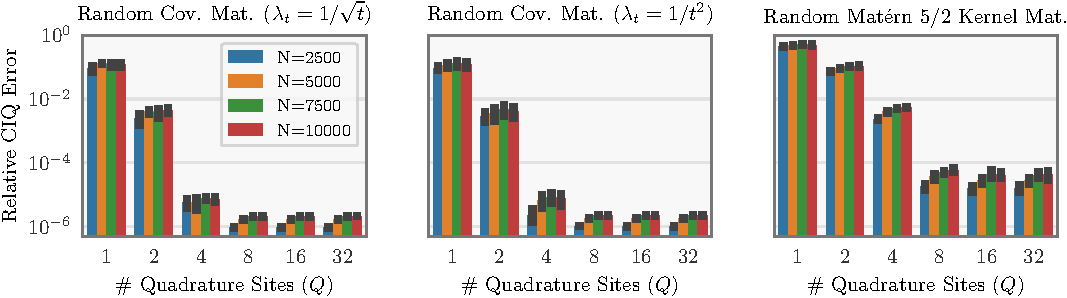
\includegraphics[width=\textwidth]{figures/quad_error.pdf}

	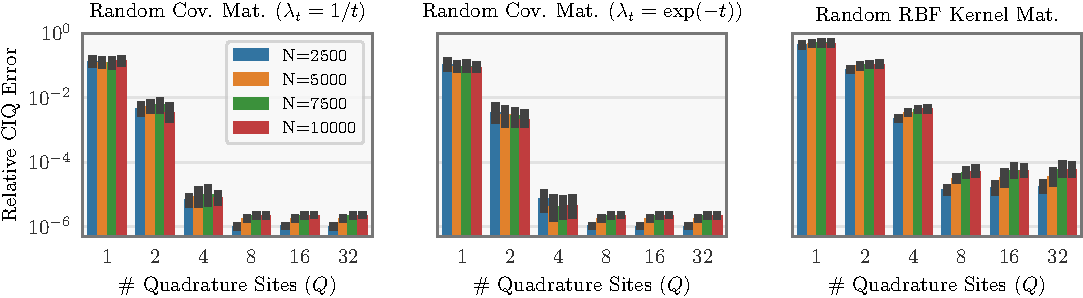
\includegraphics[width=\textwidth]{figures/quad_error_supp.pdf}
  \caption[
    Relative error of CIQ as a function of number of quadrature points $Q$.
  ]{
    CIQ relative error at computing $\bK^{1/2} \bb$ as a function of number of quadrature points $Q$.
    We test random matrices with eigenvalues that scale as $\lambda_t = 1/\sqrt{t}$ (top left), $\lambda_t = 1/t$ (bottom left), $\lambda_t = 1/{t}^2$ (top middle), and $\lambda_t = e^{-t}$ (bottom middle).
    Additionally, we test random Mat\'ern/RBF kernel matrices (top right/bottom right).
    In all cases $Q=8$ achieves $<10^{-4}$ error.
  }
  \label{fig:quad_error}
\end{figure}

Typically $J=100$ msMINRES iterations suffices for convergence; however this number can be lowered with preconditioning.
To demonstrate this, we construct  random $N \times N$ Mat\'ern/RBF kernels $\bK$, applying CIQ to a set of $N$ orthonormal vectors ($[\bK^{1/2} \bb_{1}, \ldots, \bK^{1/2} \bb_{N}]$), and compute the empirical covariance.
In \cref{fig:precond_result} we plot the number of msMINRES iterations needed to achieve a relative error of $10^{-6}$.
The pivoted Cholesky preconditioner of \cref{sec:preconditioning}---which forms a low-rank approximation of $\bK$---accelerates convergence of msMINRES.
Without preconditioning (i.e. rank=0), $J=100$ iterations are required for $N=7,\!500$ matrices.
With rank-100/rank-400 preconditioners, iterations are cut by a factor of two/four.

\begin{figure}[t!]
	\centering
	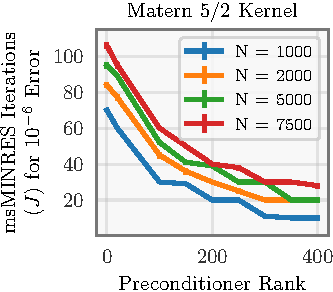
\includegraphics[width=0.4\textwidth]{figures/precond_result.pdf}
  \quad
	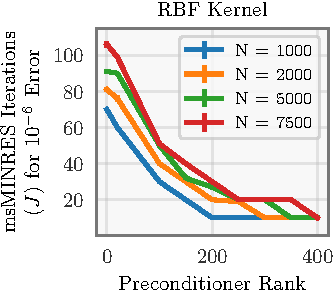
\includegraphics[width=0.4\textwidth]{figures/precond_result_rbf.pdf}
  \caption[
    Effect of preconditioning on CIQ convergence.
  ]{
    Effect of preconditioning on CIQ convergence (random Mat\'ern and RBF kernels with a pivoted Cholesky preconditioner \citep{gardner2018gpytorch}).
    Larger preconditioners reduce the number of msMINRES iterations required to reach $10^{-6}$ error.
  }
  \label{fig:precond_result}
\end{figure}

\begin{figure}[t!]
	\centering
	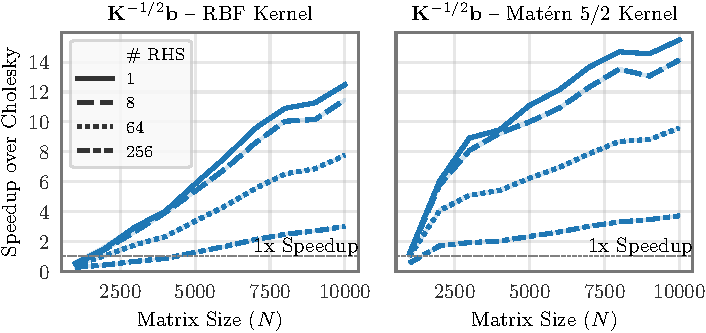
\includegraphics[width=0.8\textwidth]{figures/timing.pdf}
  \caption[
    Speedup of CIQ over Cholesky.
  ]{
    Speedup of CIQ over Cholesky when computing forward/backward passes of $\bK^{-1/2} \bb$ with varying number of right-hand-sides (RHS).
  }
  \label{fig:timing}
\end{figure}

\paragraph{Speedup over Cholesky.}
We compare the wall-clock speedup of CIQ over Cholesky in \cref{fig:timing} on RBF/Mat\'ern kernels.\footnote{
  $Q=8$.
  msMINRES is stopped after a residual of $10^{-4}$.
  Kernels are formed from the Kin40k dataset \citep{asuncion2007uci}.
  Timings are performed on a NVIDIA 1070 GPU.
}
We compute $\bK^{-1/2} \bb$ and its derivative on multiple right-hand-size (RHS) vectors.
As the $N$ increases, CIQ incurs a larger speedup (up to $15\times$ faster than Cholesky).
This speedup is less pronounced when computing many RHSs simultaneously, as the cubic complexity of Cholesky is amortized across each RHS.
Nevertheless, CIQ is computationally advantageous for matrices larger than $N=3,\!000$ even when simultaneously whitening $256$ vectors.

\section{Applications}

In the previous sections we demonstrate, both theoretically and empirically, that CIQ accurately computes $\bK^{-1/2} \bb$ and $\bK^{1/2} \bb$ while scaling better than traditional (Cholesky-based) methods.
In this section we demonstrate applications of this increased speed and scalability.
In particular, we show that using CIQ in conjunction with variational Gaussian processes and Bayesian optimization facilitates higher-fidelity models that can be applied to large-scale problems.

\subsection{Whitened Stochastic Variational Gaussian Processes}
\label{sec:variational_results}

As a first application, we will demonstrate that the CIQ whitening procedure $\bK^{-1/2} \bb$ can increase the fidelity of {\bf stochastic variational Gaussian processes (SVGP)} \cite{hensman2013gaussian,hensman2015scalable,matthews2017scalable}.
%The whitening operation is commonly used with variational approximations to accelerate the learning of variational parameters.
%
%\paragraph{Stochastic variational Gaussian process inference}
These models are used for non-conjugate likelihoods (e.g. GP classification) or for large datasets that do not fit into memory.
As described in \cref{sec:variational}, SVGP forms an approximate posterior
\[
  p(f(\bx) \mid \bX, \by) \approx q(f(\bx)) = \Evover{q(\bu)}{ p\left( f(\bx) \mid \bu \right)},
\]
where $\bu \in \reals^M$ are {inducing function values}.
$q \left( \bu \right)$ is a variational Gaussian distribution parameterized by mean $\bmm \in \reals^M$ and covariance $\bS \in \reals^{M \times M}$.
$\bmm$ and $\bS$ (as well as the model's kernel/likelihood hyperparameters) are chosen to optimize the variational ELBO:
%
\begin{align*}
  -\loglik_\text{ELBO}\Bigl\{ \bmm, \bS \Bigr\} &= -\sum_{i=1}^N \Evover{q(f(\bx^{(i)}))}{  \: \log p( y^{(i)} \mid f(\bx^{(i)}) ) \: } + \kl{ q(\bu) }{ p(\bu) }.
\end{align*}
As stated in \cref{sec:variational}, the ELBO factorizes over all data points in the training set $\bX, \by$.
Therefore, it can be approximated using minibatches and used in conjunction with stochastic gradient optimization.

Rather than directly learning $\bmm$ and $\bS$, it is more common to learn the \emph{whitened parameters} \cite{kuss2005assessing,matthews2017scalable}:
$ \bmm' = \bK_{\bZ\bZ}^{- 1/ 2} \bmm$ and $\bS' = \bK_{\bZ\bZ}^{-1 / 2} \bS \bK_{\bZ\bZ}^{-1 / 2}. $
Under these coordinates, the KL divergence term is
\[ \frac{1}{2} ( \bmm^{\prime \top} \bmm' + \tr{ \bS' } - \log \vert \bS' \vert - M ),\]
%
which doesn't depend on $p(\bu)$ and therefore is relatively simple to optimize.
The posterior distribution $q(f(\bx)) = \normaldist{\ameantest{\bx}}{\avartest{\bx}}$ is given by
%
\begin{equation}
  \begin{split}
  \ameantest{\bx} &= \bk_{\bZ\bx}^\top \bK_{\bZ\bZ}^{-\frac 1 2} \bmm',
  \\
  \avartest{\bx} &= k(\bx, \bx) -
    \bk_{\bZ\bx}^\top \bK_{\bZ\bZ}^{-\frac 1 2} \left( \bI - \bS' \right) \bK_{\bZ\bZ}^{-\frac 1 2} \bk_{\bZ\bx}.
  \end{split}
  \label{eqn:approx_pred_dist}
\end{equation}

\paragraph{Time and space complexity.}
During training, we repeatedly compute the ELBO and its derivative, which requires computing \cref{eqn:approx_pred_dist} and its derivative for a minibatch of data points.
Optimization typically requires up to $10,\!000$ iterations of training \citep[e.g.][]{salimbeni2018natural}.
We note that $\bK_{\bZ\bZ}^{-1 / 2} \bb$ (and its derivative) is the most expensive numerical operation during each ELBO computation.
If we use Cholesky to compute this operation, the time complexity of SVGP training is $\bigo{M^3}$.
On the other hand, CIQ-based SVGP training is only $\bigo{J M^2}$, where $J$ is the number of msMINRES iterations.
Both methods require $\bigo{M^2}$ storage for the $\bmm'$ and $\bS'$ parameters.

\paragraph{Natural gradient descent with CIQ.}
The size of the variational parameters $\bmm'$ and $\bS'$ grows quadratically with $M$.
This poses a challenging optimization problem for standard gradient descent methods.
To adapt to this parameter increase, we rely on {\bf natural gradient descent (NGD)} to optimize $\bmm'$ and $\bS'$ \citep[e.g.][]{hensman2012fast,salimbeni2018natural}.
At a high level, these methods perform the updates $[\bmm, \:\: \bS] \gets [\bmm, \:\: \bS] - \varphi \: \bFS^{-1} \: \nabla \loglik_\text{ELBO}$,
where $\varphi$ is a step size, $\nabla \loglik_\text{ELBO}$ is the ELBO gradient, and $\bFS$ is the {Fisher information matrix} of the variational parameters.
%\citet{salimbeni2018natural} find that NGD updates on $\bmm'$ and $\bS'$ allow for faster optimization than single-order optimizers.
%
Na\"ively, each NGD step requires $\bigo{M^3}$ computations with $\bmm'$ and $\bS'$ which would dominate the cost of CIQ-based SVGP.
Fortunately, we can derive a natural gradient update that only relies on matrix solves with $\bS'$, which take $\bigo{J M^2}$ time using preconditioned conjugate gradients.
Therefore, using NGD incurs the same \emph{quadratic} asymptotic complexity as CIQ-SVGP.
See \cref{app:ngd} for the $\bigo{M^2}$ NGD update equations.

\paragraph{Comparison of Cholesky vs CIQ.}
We compare CIQ verses Cholesky for computing \cref{eqn:approx_pred_dist} when training SVGP models.\footnote{
  Note that Cholesky computes $\bK^{-1/2} \bb$ up to an orthogonal rotation, which is suitable for whitened SVGP.
}
We test on 3 large-scale spatial datasets: a GIS dataset ({\bf 3droad}, $D=2$), a monthly precipitation dataset ({\bf Precipitation}, $D=3$), and a tree cover dataset ({\bf Covtype}, $D=54$).
Each task has between $N=70,\!000$ and $N=500,\!000$ training data points.
For 3droad we use a Gaussian observation model.
The Precipitation dataset has noisier observations; therefore we apply a Student-T observation model.
Finally, we reduce the CovType dataset to a binary classification problem and apply a Bernoulli observation model.\footnote{
  The task is predicting whether the primary tree cover at a given location is pine trees or other types of trees.
}
We train models with $M$ ranging between $1,\!000$ to $10,\!000$.

\paragraph{Experimental Details.}
Each dataset is randomly split into $75\%$ training, $10\%$ validation, and $15\%$ testing sets; $\bx$ and $y$ values are scaled to be zero mean and unit variance.
All models use a constant mean and a Mat\'ern 5/2 kernel, with lengthscales initialized to $0.01$ and inducing points initialized by $K$-means clustering.
Each model is trained for $20$ epochs with a minibatch size of $256.$\footnote{
  The batch size is $512$ on the Covtype dataset due to its larger size.
}
We alternate between optimizing $\bmm'/\bS'$ and the other parameters, using natural gradient descent for the former and Adam \cite{kingma2014adam} for the latter.
Each optimizer uses an initial learning rate of $0.01$\footnote{
  On the Precipitation dataset, we use an initial learning rate of $0.005$ for  NGD stability with the Student-T likelihood.
}, decayed by $10\times$ at epochs $1$, $5$, $10$, and $15$.
For CIQ we use $Q = 15$ quadrature points.
MINRES terminates when the $\bc_j$ vectors achieve a relative norm of $0.001$ or after $J=200$ iterations.

%\paragraph{Training time.}
%In \cref{fig:variational_timing_and_stats} (left) we plot the training time (in hours) of CIQ/Cholesky models as a function of $M$.
%Each model is trained for $20$ epochs on a single NVIDIA Titan-RTX GPU.
%Both the Cholesky and CIQ variants take increasingly longer to train as $M$ increases.
%Nevertheless, we observe that CIQ models are able to scale to larger $M$ values under a fixed computational budget.
%Both CIQ and Cholesky take roughly the same amount of time for $M=1,\!000$ inducing points.
%However, CIQ models are roughly $4\times$ faster at $M=5,\!000$.
%On the Precipitation dataset, a CIQ model with $M=10,\!000$ finishes training faster than a Cholesky model with $M=5,\!000$.

\begin{figure}[t!]
  \centering
  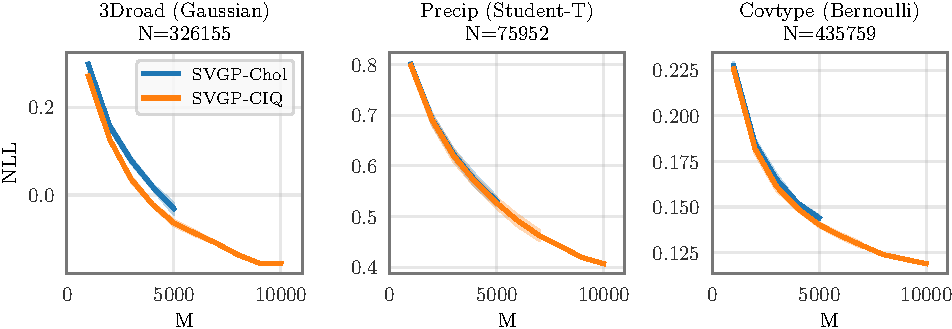
\includegraphics[width=\linewidth]{figures/variational_nll.pdf}
  \caption[Negative log likelihood (NLL) comparison of Cholesky-whitened vs CIQ-whitened SVGP models.]{
    Negative log likelihood (NLL) comparison of Cholesky vs CIQ SVGP models.
    {\bf Left:} 3DRoad dataset ($N=326155, D=2$, Gaussian likelihood).
    {\bf Middle:} Precipitation dataset ($N=75952, D=3$, Student-T likelihood).
    {\bf Right:} CoverType dataset ($N=435759, D=54$, Bernoulli likelihood).
    NLL improves with inducing points ($M$); Cholesky and CIQ models have similar performance.
    However CIQ models train faster than their Cholesky counterparts.
  }
  \label{fig:variational_nll}
\end{figure}

\begin{figure}[t!]
  \centering
  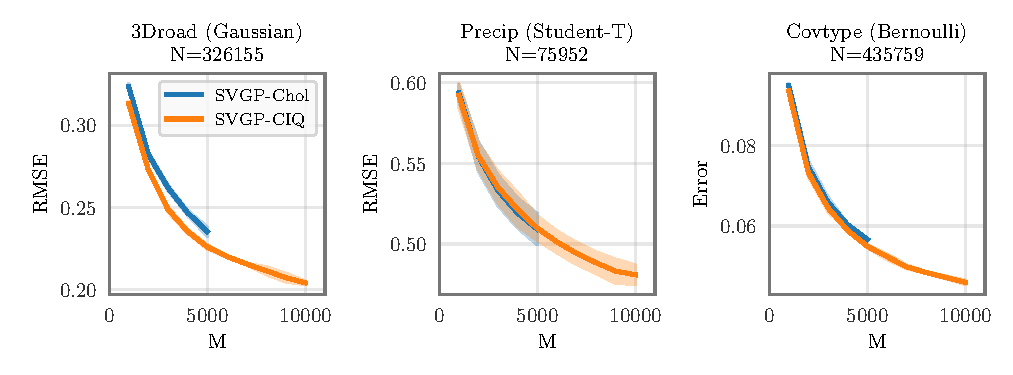
\includegraphics[width=\linewidth]{figures/variational_error.pdf}
  \caption[Error comparison of Cholesky-whitened vs CIQ-whitened SVGP models.]{
    Error comparison of Cholesky-whitened vs CIQ-whitened SVGP models.
    {\bf Left:} 3DRoad dataset RMSE ($N=326155, D=2$, Gaussian likelihood).
    {\bf Middle:} Precipitation dataset RMSE ($N=75952, D=3$, Student-T likelihood).
    {\bf Right:} CoverType dataset $0/1$ error ($N=435759, D=54$, Bernoulli likelihood).
  }
  \label{fig:variational_error}
\end{figure}

\paragraph{Results.}
The computations of $\bK_{\bZ\bZ}^{-1/2} \bk_{\bZ\bx}$ from CIQ and Cholesky are the same up to an orthogonal rotation.
However, adaptive gradient optimizers (which we use for the kernel/likelihood hyperparameters) are not invariant to orthogonal transformation.
While CIQ and Cholesky SVGP models may learn different parameters, the two methods achieve very similar test-set negative log likelihood (\cref{fig:variational_nll}) and predictive error (\cref{fig:variational_error}).
%On 3droad, CIQ models tend to slightly outperform Cholesky models.
The key difference is the training time:
with $M=5,\!000$ inducing points, CIQ models are up to \emph{5.6 times faster} than Cholesky models (as measured on a Titan RTX GPU).
Moreover, CIQ models with $M=8,\!000$-$10,\!000$ take roughly the same amount of time as $M=5,\!000$ Cholesky models.
We do not train $M > 5,\!000$ Cholesky models as such these would require $2$-$10$ days for training.

\begin{figure}[t!]
  \centering
  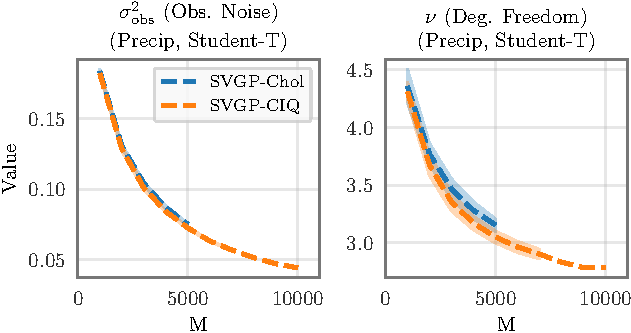
\includegraphics[width=\linewidth]{figures/variational_stats.pdf}
  \caption[Train time comparison of Cholesky-whitened vs CIQ-whitened SVGP models.]{
    Hyperparameters verses number of inducing points ($M$) for Chol-SVGP and CIQ-SVGP (Precipitation dataset, Student-T likelihood).
    As $M$ increases, the kernel outputscale (left) also increases.
    At the same time, the estimated observational noise (middle) decreases as does the estimated degrees of freedom (right), reflecting a heavier-tailed noise distribution.
    This suggests that, with larger $M$, SVGP models can find more signal in the data.
  }
  \label{fig:variational_stats}
\end{figure}

\paragraph{Effects of increased inducing points.}
We find that accuracy improves with increased $M$ on all datasets.
Scaling from $M=5,\!000$ to $M=10,\!000$ reduces test-set NLL by $0.1$ nats on the 3droad and Precipitation datasets.
We find similar reductions in predictive error (\cref{fig:variational_error} for plots).
By scaling more readily to large $M$, CIQ enables high-fidelity variational approximations that would be computationally prohibitive with Cholesky.

We also find that increasing $M$ changes the values of the learned kernel/likelihood hyperparameters.
In \cref{fig:variational_stats} we plot the learned hyperparameters of the Precipitation SVGP models:
%
\begin{enumerate*}
  \item $o^2$ (the kernel outputscale)---which roughly corresponds to variance explained as ``signal'' in the data;
  \item $\sigma^2_\text{obs}$---which roughly corresponds to variance explained away as observational noise; and
  \item $\nu$ (degrees of freedom)---which controls the tails of the noise model (lower $\nu$ corresponds to heavier tails).
\end{enumerate*}
%
As $M$ increases, we find that the observational noise parameter decreases by a factor of $4$---down from $0.19$ to $0.05$---while the $\nu$ parameter also decreases.
Models with larger $M$ values can more closely approximate the true posterior \cite{hensman2013gaussian}; therefore, we expect that the larger-$M$ likelihoods more closely correspond to the true parameters.
This confirms findings from \citet{bauer2016understanding}, who argue that variational approximations with small $M$ tend to overestimate the amount of noise in datasets.

\section{Application 2: Posterior Sampling for Bayesian Optimization}
\label{sec:sampling_results}

The second application of CIQ we explore is GP posterior sampling in the context of Bayesian optimization \citep[e.g.][]{snoek2012practical}.
Bayesian optimization methods aim to find the maximum (or minimum) of a black-box function $g(\cdot)$
(e.g. $g(\cdot)$ is the validation error of a neural network as a function of hyperparameters).
A Gaussian process $f(\cdot)$ is typically used as a surrogate model, modelling the probabilistic beliefs about $g(\cdot)$ based on previous observations $\dset_N = (\bx_1, g(\bx_1)), \ldots, (\bx_N, g(\bx_N))$ (e.g. previous hyperparameter configurations).
At each iteration, we select a new point acquisition point $\bx_{N+1}$; we evaluate $g(\bx_{N+1})$; and then we update our posterior belief over $f$.

To select the new point $\bx_{N+1}$, we evaluate an {\bf acquisition function} at many possible candidate points $\mathcal{T} = \{ \bxtest_1, \ldots, \bxtest_T \}$.
Intuitively, an acquisition functions determines how useful it would be to evaluate $g(\bxtest_i)$.
Many acquisition functions require drawing samples from the current GP posterior $p(f(\bxtest_1), \ldots, f(\bxtest_T) \mid \dset)$.
One canonical example is {\bf Thompson Sampling} \cite{thompson1933likelihood}, which trades off exploitation of existing minima for exploration of new potential minima.
Thompson sampling simply chooses $\bx_N$ as the minimizer of a sample $f(\cdot)$ drawn from the posterior.
%
\[
  \bx^\text{(Thompson)}_{N+1} = \argmin_{\bx_i \in \mathcal{T}} f(\bx_i),
  \quad
  f(\cdot) \sim p(f(\cdot) \mid \dset_N).
\]
%
Let $\bmeantest \in \reals^{T}$ and $\Covtest \in \reals^{T \times T}$ be the posterior mean and covariance evaluated at $\bxtest_1$, $\ldots$, $\bxtest_T$.
For each iteration of Thompson sampling we draw a sample via
%
\begin{equation}
  \meantest + {\Covtest}^{\frac 1 2} \bepsilon,
  \quad
  \bepsilon \sim \normaldist{\bzero}{\bI}.
  \label{eqn:thompson_sample}
\end{equation}
%
In many Bayesian optimization, the candidate points $\bxtest_1$, $\ldots$, $\bxtest_T$ are uniformly sampled in the search space \cite{balandat2019botorch}.
Larger values of $T$ more densely cover the search space, which naturally should result in better acquisition points.
It is therefore beneficial to choose the largest value of $T$ that is computationally feasible.
Using Cholesky to compute \cref{eqn:thompson_sample} incurs a $\bigo{T^3}$ cost which severely limits the size of $T$.
On the other hand, CIQ is only $\bigo{T^2}$, can be preconditioned, and more readily utilizes GPU acceleration.
When used in the conjunction with kernel partitioning methods that will be described in the next chapter, the memory requirement of CIQ can also be reduced to $\bigo{N}$ (see \cref{sec:largeexact_method}).


\subsection{Results}

We perform Bayesian optimization on three high-dimensional black-box functions: a classical test function ({\bf Hartmann}, $D=6$) and two robotics simulations ({\bf Lunar Lander}, $D=12$; {\bf Rover}, $D=60$).
For each problem we use exact Gaussian processes (no approximations) as the surrogate model and Thompson sampling as the acquisition function.
Our goal is to determine whether CIQ-based sampling is beneficial by allowing us to scale to larger candidate set sizes.

\paragraph{Baselines.}
Here, we limit the baseline methods to exact sampling methods, and therefore do not consider stochastic approximations \cite{rahimi2008random} or methods that rely on inducing points \cite{wilson2020efficiently}.
Consequentially, we do not compare against LOVE-based sampling from \cref{chapter:love} as its can only be used in conjunction with the KISS-GP approximation.
It is worth noting that, with sufficient quadrature points and msMINRES iterations, we can reduce the error of CIQ to machine precision (see \cref{thm:ciq_convergence}); therefore it can be considered an exact sampling method like Cholesky.

\begin{figure}[t!]
  \centering
  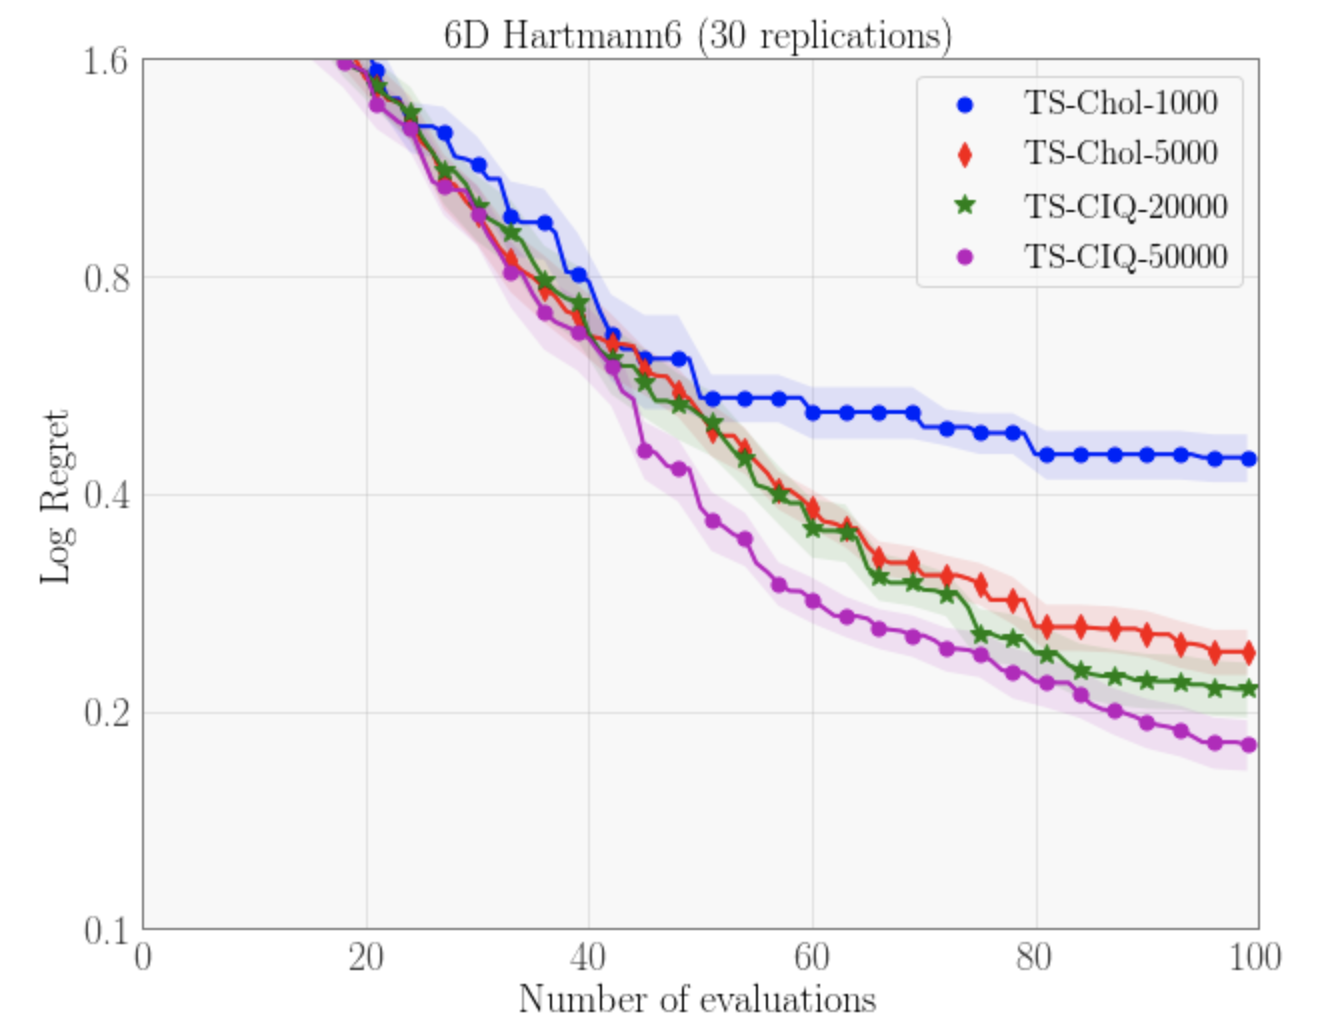
\includegraphics[width=0.72\linewidth]{figures/hartmann6.png}
  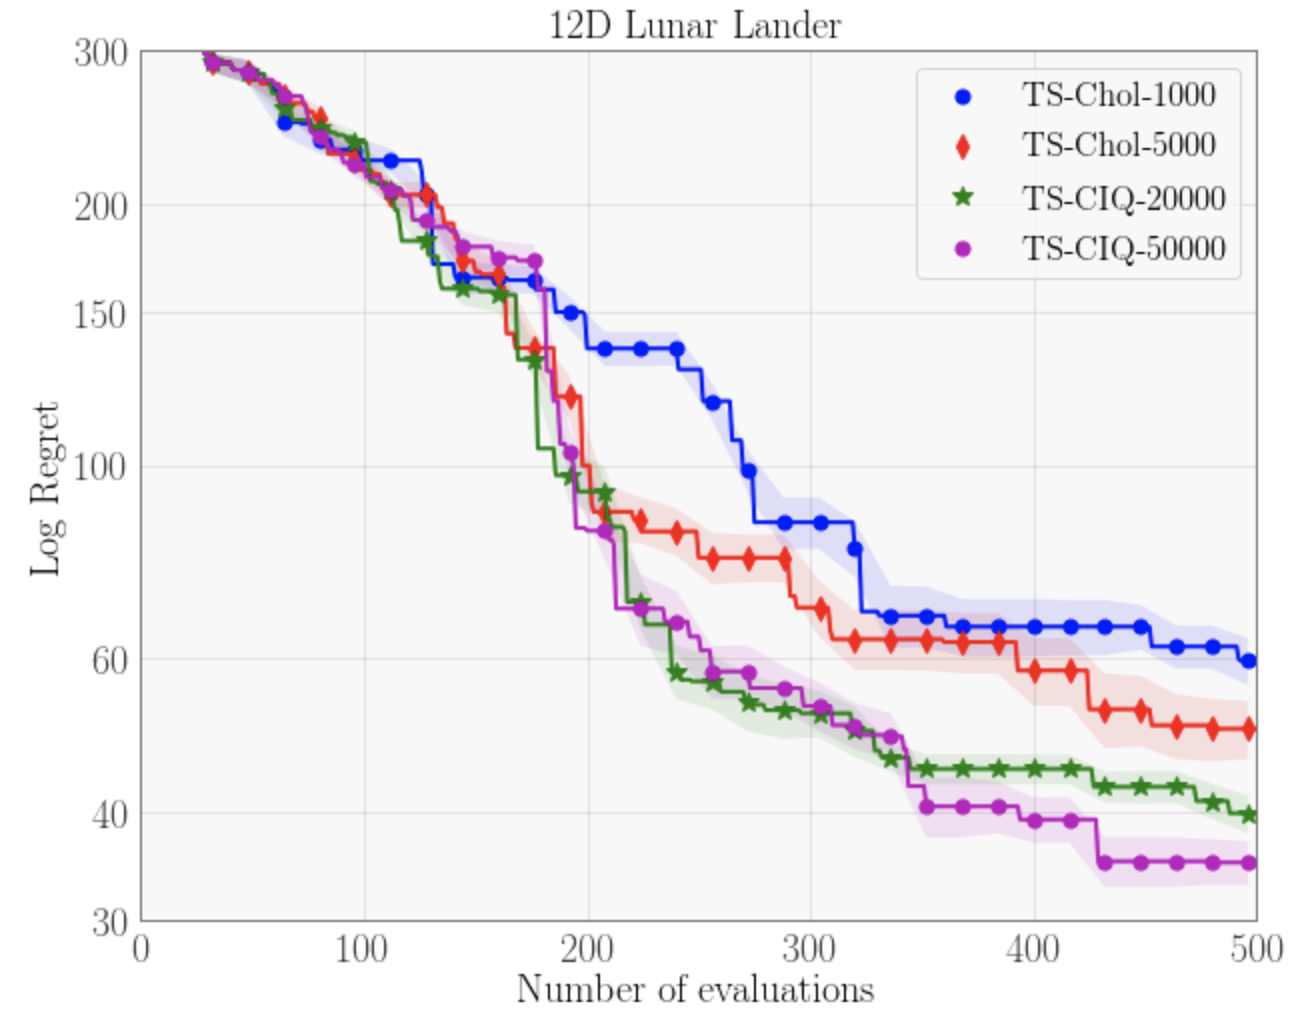
\includegraphics[width=0.7\linewidth]{figures/lunar_lander.png}
  \caption[
    A comparison of sampling methods for Bayesian optimzation (BayesOpt) via Thompson sampling.
    BayesOpt is applied to the Hartmann ($D=6$) and Lunar Lander ($D=12$) functions.
  ]{
    A comparison of sampling methods for Bayesian optimzation (BayesOpt) via Thompson sampling.
    BayesOpt is applied to the ({\bf top}) Hartmann ($D=6$) and ({\bf bottom}) Lunar Lander ($D=12$) functions.
    Methods: TS-Chol-$\langle T \rangle$ draws posterior samples with Cholesky at $T$ candidate points.
    TS-CIQ-$\langle T \rangle$ draws posterior samples with CIQ.
    Larger $T$ (number of candidate point) results in better optimization.
    CIQ enables scaling to $T\geq50,\!000$.
  }
  \label{fig:hartmann6_lunar}
\end{figure}

We measure the performance of Thompson sampling as a function of the candidate set size $T$.
We run Thompson sampling Bayesian optimization with $T=1,\!000$, $T=5,\!000$, $T=20,\!000$, and $T=50,\!000$.
We use Cholesky ({\bf TS-Chol}) for $T=1,\!000$ and $T=5,\!000$, and we use CIQ ({\bf TS-CIQ}) for $T=20,\!000$ and $T=50,\!000$.
Note that it would be very challenging and impractical to use Cholesky with $T\geq10,\!000$, both due to its quadratic memory and its cubic time complexity.

\paragraph{Experimental details.}
The Gaussian processes use RBF kernels and zero mean functions.
After each posterior update, we optimize the GP hyperparameters using 10 iterations of Adam with a learning rate of $0.1$.
The candidate sets are sampled uniformly at random from the input space.
As with the variational experiments, we use $Q = 15$ quadrature points for CIQ.
MINRES terminates when the $\bd_j$ vectors achieve a relative norm of $0.001$ or after $J=1,\!000$ iterations.
We use a partial pivoted Cholesky preconditioner of rank $R=20$ when drawing CIQ samples.

For the Hartmann and Lunar Lander problems we use standard Thompson sampling acquisition function.
At each iteration we draw 5 posterior samples and choose the acquisition point based on the minimum of all samples.
Due to the high-dimensionality of the Rover problem, we use Thompson sampling in conjunction with the trust-region BayesOpt method of \citet{eriksson2019scalable}.
We use separate candidate sets for each trust region, and similarly choose the next acquisition point based on 5 posterior samples.

\begin{figure}[t!]
  \centering
  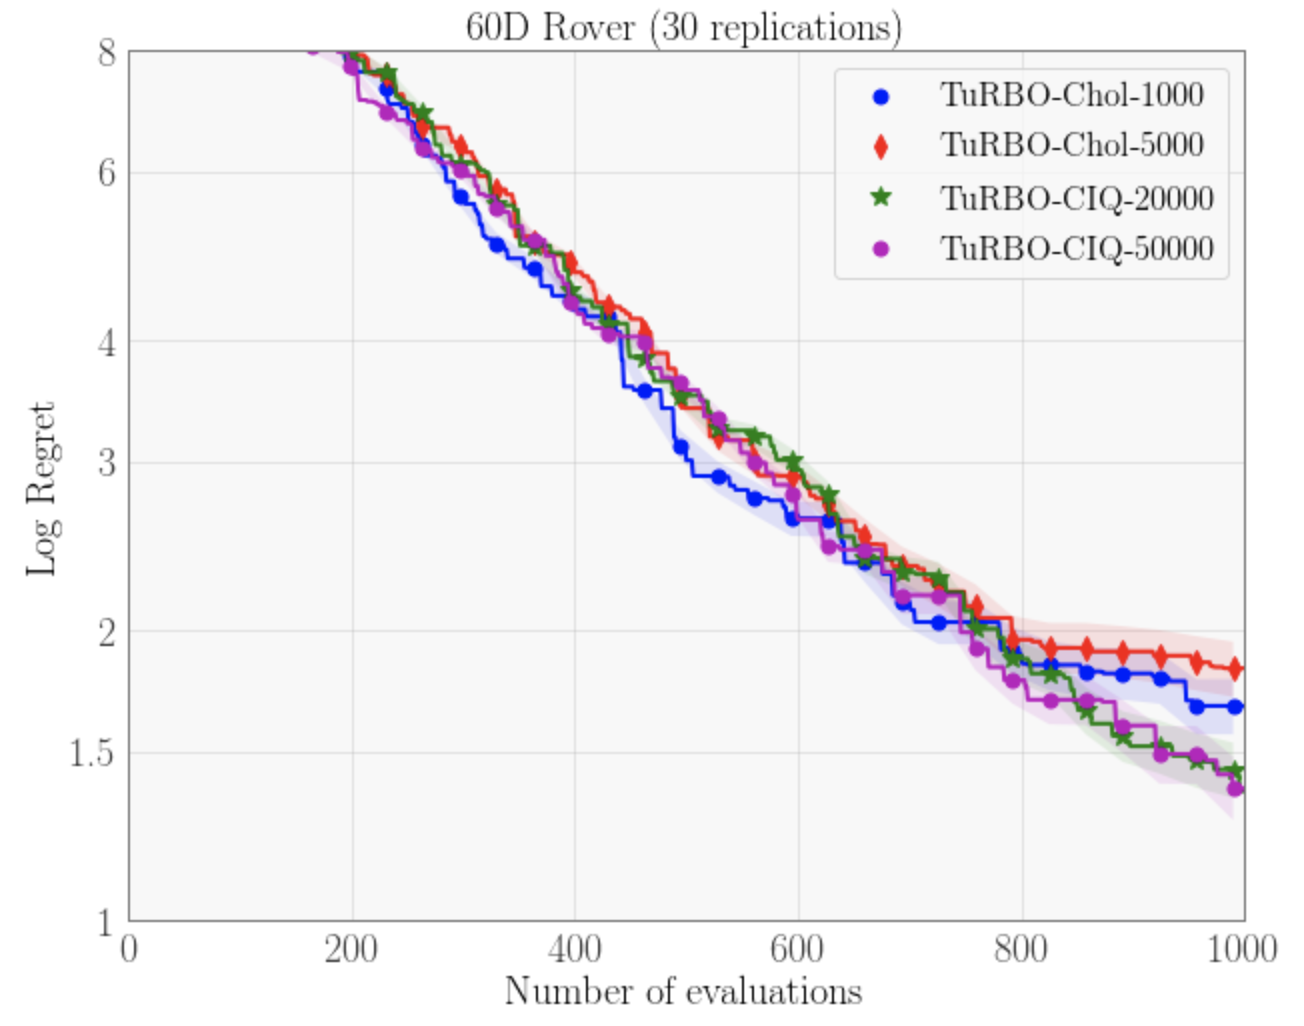
\includegraphics[width=0.7\linewidth]{figures/rover.png}
  \caption[
    A comparison of sampling methods for Bayesian optimzation (BayesOpt) via TuRBO \cite{eriksson2019scalable}.
    BayesOpt is applied to the Rover ($D=60$) function.
  ]{
    A comparison of sampling methods for Bayesian optimzation (BayesOpt) via TuRBO \cite{eriksson2019scalable}.
    BayesOpt is applied to the Rover ($D=60$) function.
    Larger $T$ (number of candidate point) results in better optimization.
    CIQ enables scaling to $T\geq50,\!000$, whereas Cholesky is limited to $T\leq5,\!000$
  }
  \label{fig:rover}
\end{figure}

\paragraph{Optimization performance.}
We plot the log regret of the Thompson sampling variants (Harmann and Lunar Lander in \cref{fig:hartmann6_lunar}, Rover in \cref{fig:rover}).
From these figures we can make several observations.
At early stages of optimization, the log regret is similar for all candidate set sizes.
However, in later stages of optimization we notice that larger candidate set sizes begin to have much lower regret.
By increasing $T=1,\!000$ to $T=50,\!000$, we cut the final log regret by substantial amounts on all problems.
On the Hartmann and Lunar Lander problems, we even see improved performance as we increase $T$ from $20,\!000$ to $50,\!000$.
It is therefore likely that even larger candidate set sizes could further improve optimization.

We re-iterate that $T=50,\!000$ is largely impractical with Cholesky sampling methods.
Large candidate sets have previously only been possible with approximate sampling methods.
CIQ enables us to scale to much larger values of $T$ without incurring additional bias or variance.

\section{Discussion}

We have introduced msMINRES-CIQ---a MVM-based method for computing $\bK^{1/2} \bb$ and $\bK^{-1/2} \bb$.
In sampling and whitening applications, msMINRES-CIQ can be used as a $\bigo{N^2}$ drop-in replacement for the $\bigo{N^3}$ Cholesky decomposition.
Its scalability and GPU utilization enable us to use more inducing points with SVGP models and larger candidate sets in Bayesian optimization.
In all applications, such increased fidelity results in better performance.


\paragraph{Advantages and disadvantages.}
One advantage of the Cholesky decomposition is its reusability.
As discussed in \cref{sec:ciq_empirical}, the cubic cost of computing $\bL \bL^\top$ is amortized when drawing $\bigo{M}$ samples or whitening $\bigo{M}$ vectors.
Conversely, applying msMINRES-CIQ to $\bigo{M}$ vectors would incur a $\bigo{M^3}$ cost, eroding its computational benefits. Thus, our method is primarily advantageous
in scenarios with a small number of right hand sides or where $\bK$ is too large to apply Cholesky.
We also emphasize that msMINRES-CIQ---like all Krylov methods---can take advantage of fast MVMs.
Though this chapter focuses on applying this algorithm to dense matrices, we suggest that future work explore applications involving sparse or structured matrices.


\paragraph{Scaling beyond $M=10,\!000$ and $T=50,\!000$.}
It has been common to use only $M\approx1,\!000$ inducing points with SVGP models.
In this chapter, we have used \emph{an order of magnitude} more inducing points which results in demonstrably better predictive performance.
As $M$ continues to grow, the primary bottleneck of msMINRES-CIQ-SVGP becomes the quadratic memory costs of the variational parameters $\bm'$ and $\bS'$.
While a scalable approximation of $\bK_{\bZ\bZ}$ (with fast MVMs) can reduce the computational cost of whitening, the $\bS'$ matrix in general does not afford space-saving structure.
Efficient variational parameterizations will be necessary to scale to even larger $M$.
This has been the topic of some recent work \cite{wilson2016stochastic,cheng2017variational,salimbeni2018orthogonally,shi2019sparse}.

Scaling msMINRES-CIQ Thompson sampling beyond $T=50,\!000$ is to some extent more straightforward, as it does not require storing learnable parameters.
%One option is to use Thompson sampling in conjunction with approximate GP methods that afford faster MVMs.
%However, choosing a suitable approximate method may be difficult when modelling blackbox functions without knowing much prior structure.
Nevertheless, scaling $T$ will naturally require more computation, which may result in the acquisition function becoming increasingly computationally demanding.
The next section introduces a simple strategy to utilize multiple GPUs/distributed resources to alleviate this bottleneck.


\chapter{Scaling Exact Gaussian Processes to Millions of Data Points}

\chapter{Conclusion and Future Directions}
\label{chapter:discussion}


This thesis has presented a comprehensive framework for Gaussian process training, inference, and prediction.
The algorithms proposed in \cref{chapter:bbmm,chapter:love,chapter:ciq} are based around a single central design decision: reduce all expensive matrix operations to parallelized matrix-vector multiplications (MVMs).
\cref{chapter:bbmm} introduced the Black-Box Matrix~\texttimes~Matrix (BBMM) framework which computes GP training terms via a modified batched-conjugate gradients algorithm (mBCG).
To enable fast predictions with GP models, \cref{chapter:love} presented LanczOs Variance Estimates (LOVE), which computes an amortized cache of the predictive posterior.
Finally, \cref{chapter:ciq} introduced Cauchy Integral Quadrature (CIQ) to ``whiten'' and ``unwhiten'' vectors with respect to a Gaussian covariance---enabling
the MVM-based training of variational GP models and also allowing efficient posterior sampling.

The MVM theme simultaneously addresses several desiderata for Gaussian processes.
As demonstrated in \cref{chapter:bbmm}, MVM-based methods effectively utilize GPU hardware and reduce specialty implementations to $\leq 50$ lines of code.
This makes it easy for researchers to rapidly prototype and test novel models across a wide variety of datasets.
%MVM-based methods also reduce the asymptotic complexity of GPs, which in turn allows for in more powerful predictions and inferences.
MVM-based methods also lead to faster, more powerful models.
\cref{chapter:love} significantly reduces computational costs of GPs at test-time, while
\cref{chapter:ciq} scales up variational approximations and large-scale sampling, leading to better predictions and black-box optimization.
Combined, these methods expand what is considered tractable for exact GPs, as demonstrated in the $N=1,\!000,\!000$ experiments of \cref{chapter:largeexact}.
\clearpage



\section{Beyond Matrix-Vector Multiplication}

The framework presented in this thesis makes GPs increasingly practical on massive datasets.
%Moreover, standard GP models can be an effective model class for many large datasets (as demonstrated in \cref{sec:largeexact_results}).
Large-scale problems allow for more powerful classes of GP-based models, which in turn opens up many exciting research problems.
%These problems go beyond the scope of what is addressed by the MVM methods in this thesis.

To increase the representational capacity of Gaussian processes, researchers have proposed highly-parametric kernels \cite{wilson2013gaussian,wilson2016stochastic}, using GPs as components of larger pipelines \cite{schulam2015framework,futoma2017learning}, and hierarchical GP models \cite{wilson2012gaussian,salimbeni2017doubly,jankowiak2020deep}.
%These models are an attractive choice for large-scale modelling: combining the expressively and capacity of techniques like deep learning with the probabilistic capabilities afforded by Gaussian processes.
Of course, the additional complexity of these approaches may pose new training and inference challenges.
Advances in large-scale optimization have mostly targeted the piece-wise linear geometry of ReLU neural networks and may need to be adapted to the geometry of Gaussian processes-based models.
This is especially true for GP models that use alternative objective functions for learning \cite{sheth2017excess,knoblauch2019generalized,jankowiak2020parametric}.
Moreover, hierarchical GP models are more computationally intensive than simpler models.
%Deep Gaussian processes for example stack multiple GPs on top of one another, and BBMM-style methods should be adapted to handle this sequential computation.
Such models necessitate parametric approximations, as exact inference is intractable.
Consequentially, increasing the fidelity of these models (e.g. stacking more layers, using more inducing points) increases the number of parameters, which may become an optimization or test-time bottleneck.
It is worth noting that these problems are not unique to large-scale Gaussian processes---they are also issues of other large-scale machine learning models.
Addressing these challenges in the context of GPs however is a relatively new area of research, as these models have only recently been considered practical.




\section{Beyond Gaussian Processes}

A key insight of this thesis is that non-linear operations on large-scale kernel matrices are surprisingly tractable when used in conjunction with GPU acceleration and efficient numerical techniques.
While we motivate this finding through GPs, it is worth noting that the algorithms presented here are applicable to other classes of models.
For example, a common relaxation to optimal transport problems is solved via Sinkhorn iterations \cite{cuturi2013sinkhorn}, which rely on iterative MVMs with an exponentiated distance matrix.
%This exponentiated distance matrix can be interpreted as a scaled RBF kernel, and therefore the preconditioning and partitioning techniques from this thesis might scale this algorithm beyond its current limits.
Second-order optimization is another application where large-scale solves are necessary.
GPU-accelerated MVM methods may make such methods applicable to higher dimensional problems \cite{koh2017understanding}.

More generally, machine learning in recent years has shied away from complex matrix operations.
Many modern algorithms instead derive expressive power through the composition of linear and element-wise functions \cite{goodfellow2016deep}.
While deep neural networks demonstrate the merit of this approach, it is possible that incorporating more complex matrix operations could improve parameter efficiency and model capacity \cite{jankowiak2020deep}.
The ability to efficiently compute arbitrary functions of big matrices opens up possibilities well beyond large-scale Gaussian process models.



\appendix

%!TEX root=../main.tex
\chapter{Details on the Convergence Analysis of Preconditioned mBCG}

\section{Proof of Theorems in Section~\ref{sec:piv_chol_precond}}
\label{app:proofs}
Here we include theorems and proofs about the partial pivoted Cholesky preconditioner applied to mBCG.
All theorems are restated from \cref{sec:piv_chol_precond}.


\subsection{Proof of Lemma~\ref{thm:condition_number}}
\newtheorem*{thm:condition_number}{Lemma~\ref{thm:condition_number} (Restated)}
\begin{thm:condition_number}
  Let $\bar\bL_{R}$ be the rank-$R$ pivoted Cholesky factor of kernel matrix $\bK_{\bX\bX} \in \reals^{N \times N}$.
  If the first $R$ eigenvalues $\lambda_1$, $\ldots$, $\lambda_R$ of $\bK_{\bX\bX}$ satisfy
	\begin{equation*}
		4^{i}\lambda_{i} \leq \bigo{e^{-Bi}}, \quad i \in \{ 1, \:\: \ldots, \:\: R \},
		\tag{\ref{eqn:pcp_condition}}
	\end{equation*}
	for some $B>0$, then the condition number $\kappa(\trainP^{-1}\trainK) \triangleq \Vert \trainP_{k}^{-1}\trainK \Vert_{2} \Vert \trainK^{-1}\trainP_{k} \Vert_{2}$
	satisfies the following bound:
  \begin{align}
    \kappa \left( \trainP^{-1}\trainK \right)
    &\leq \Bigl( 1 + \bigo{\sigma^{-2}_\text{obs} N e^{-BR}} \Bigr)^2
		\nonumber
  \end{align}
	where $\trainP = \left( \bar\bL_R \bar\bL_R^\top + \sigma^2_\text{obs} \bI \right)$ and $\trainK = \left( \bK_{\bX\bX} + \sigma^2_\text{obs} \bI \right)$.
\end{thm:condition_number}

\begin{proof}
  Let $\bE$ be the difference between $\bK_{\bX\bX}$ and its rank-$R$ pivoted Cholesky approximation $\bar\bL_R \bar\bL_R^\top$:
  \[
    \bE = \bK_{\bX\bX} - \bar\bL_R \bar\bL_R^\top = \begin{bmatrix} \bzero & \bzero \\ \bzero & \bS_{R+1} \end{bmatrix}
  \]
  where $\bS_{R+1}$ is the Schur compliment that arises as the Cholesky error term---\cref{eqn:chol_error}.
  The error $\bE$ is therefore a positive semi definite matrix.

  By definition, the condition number $\kappa ( \trainP^{-1}\trainK )$ is given by
  \begin{align*}
    \kappa \left( \trainP^{-1}\trainK \right)
    &\triangleq \left\Vert \trainP^{-1}\trainK \right\Vert_{2} \left\Vert \trainK^{-1}\trainP \right\Vert_{2}
  \end{align*}
  %
  The left term can be rewritten as:
  %
  \begin{align*}
    \\
    \left\Vert \trainP^{-1}\trainK \right\Vert_{2}
    &= \left\Vert \left( \bar\bL_R \bar\bL_R^\top + \sigma^2_\text{obs} \bI \right)^{-1} \left(\bK_{\bX\bX} + \sigma^2_\text{obs} \bI \right) \right\Vert_{2}
    \\
    &= \left\Vert \left( \bar\bL_R \bar\bL_R^\top + \sigma^2_\text{obs} \bI \right)^{-1} \left(\bar\bL_R \bar\bL_R^\top + \bE + \sigma^2_\text{obs} \bI \right) \right\Vert_{2}
    \\
    &= \left\Vert \bI + \left( \bar\bL_R \bar\bL_R^\top + \sigma^2_\text{obs} \bI \right)^{-1} \bE \right\Vert_{2}
  \end{align*}
  %
  Similarly, the right term is:
  %
  \begin{align*}
    \left\Vert \trainK^{-1}\trainP \right\Vert_{2}
    &= \left\Vert \left( \bar\bL_R \bar\bL_R^\top + \sigma^2_\text{obs} \bI \right) \left(\bK_{\bX\bX} + \sigma^2_\text{obs} \bI \right)^{-1} \right\Vert_{2}
    \\
    &= \left\Vert \left( \bK_{\bX\bX} - \bE + \sigma^2_\text{obs} \bI \right) \left(\bK_{\bX\bX} + \sigma^2_\text{obs} \bI \right)^{-1} \right\Vert_{2}
    \\
    &= \left\Vert \bI - \left(\bK_{\bX\bX} + \sigma^2_\text{obs} \bI \right)^{-1} \bE \right\Vert_{2}
  \end{align*}
  %
  Since $\bK_{\bX\bX}$ and $\bar\bL_R \bar\bL_R^\top$ are both positive (semi-)definite,
  $(\bK_{\bX\bX} + \sigma^2_\text{obs})$ and $(\bar\bL_R \bar\bL_R^\top + \sigma^2_\text{obs})$ will both have a minimum eigenvalue $\lambda_\text{min} \geq \sigma^2_\text{obs}$.
  Therefore,
  %
  \[
    \left\Vert \left(\bK_{\bX\bX} + \sigma^2_\text{obs} \right)^{-1} \right\Vert_2 \leq \sigma^{-2}_\text{obs},
    \quad
    \left\Vert \left(\bar\bL_R \bar\bL_R^\top + \sigma^2_\text{obs} \right)^{-1} \right\Vert_2 \leq \sigma^{-2}_\text{obs}.
  \]
  %
  Applying these bound, along with Cauchy-Schwarz and the triangle inequality, gives us
  %
  \begin{align}
    \kappa \left( \trainP^{-1}\trainK \right) \!
    &\leq \! \left( 1 + \left\Vert \left( \bar\bL_R \bar\bL_R^\top + \sigma^2_\text{obs} \bI \right)^{-1} \right\Vert_2 \left\Vert \bE \right\Vert_{2} \right)
      \!\!
      \left( 1 + \left\Vert \left( \bK_{\bX\bX} + \sigma^2_\text{obs} \bI \right)^{-1} \right\Vert_2 \left\Vert \bE \right\Vert_{2} \right)
    \nonumber \\
    &\leq
    \left( 1 + \sigma^{-2}_\text{obs} \Vert \bE \Vert_2 \right)
    \left( 1 + \sigma^{-2}_\text{obs} \Vert \bE \Vert_2 \right)
    \nonumber \\
    &= \left( 1 + \sigma^{-2}_\text{obs} \Vert \bE \Vert_2 \right)^2.
    \label{eqn:cond_number_bound}
  \end{align}

  Since $\bE$ is positive semi-definite, we have that $\Vert \bE \Vert_2 \leq \tr{\bE}$.
  The eigenvalue condition from \cref{eqn:pcp_condition} allows us to bound $\tr{\bE}$ using \cref{thm:harbrecht}:
  %
  \begin{equation}
    \Vert \bE \Vert_2 \leq \tr{\bE}
    =
    \tr{ \bK_{\bX\bX} - \bar\bL_R \bar\bL_R^\top } \leq \bigo{N e^{-BR}}.
    \label{eqn:error_trace_bound}
  \end{equation}
  %
  Plugging \cref{eqn:error_trace_bound} into \cref{eqn:cond_number_bound} completes the proof.
\end{proof}




\subsection{Proof of Theorem~\ref{thm:precond_mbcg_solves}}
\newtheorem*{thm:precond_mbcg_solves}{\cref{thm:precond_mbcg_solves} (Restated)}
\begin{thm:precond_mbcg_solves}
  Let $\bK_{\bX\bX} \in \reals^{N \times N}$ be a $N \times N$ kernel that satisfies the eigenvalue condition of \cref{eqn:pcp_condition},
	and let $\bar\bL_R$ be its rank-$R$ pivoted Cholesky factor.
	After $J$ iterations of mBCG with preconditioner $\trainP = (\bar\bL_R \bar\bL_R^\top + \sigma_\text{obs}^2 \bI)$,
	the difference between $\bc_J$ and true solution $\trainK^{-1} \by$ is bounded by:
	%
  \begin{equation*}
    \left \Vert \trainK^{-1} \by - \bc_{J} \right \Vert_{\trainK}
    \leq \Bigg[ \frac 1 {1 + \bigo{\sigma^{2}_\text{obs} e^{RB}/N}} \Bigg]^{J}
    \left \Vert \trainK^{-1} \by \right \Vert_{\trainK},
		\nonumber
  \end{equation*}
	%
	where $\trainK = (\bK_{\bX\bX} + \sigma^2_\text{obs} \bI)$ and $B > 0$ is a constant.
\end{thm:precond_mbcg_solves}

\begin{proof}
Since \cref{eqn:pcp_condition} holds, we can simply plug \cref{thm:condition_number} into the standard CG convergence bound (\cref{thm:cg_convergence}):
%
\begin{align*}
  \left \Vert \trainK^{-1} \by - \bc_{J} \right \Vert_{\trainK}
  &\leq
  2 \left[ \frac{ \sqrt{ \kappa\left( \trainP^{-1} \trainK \right)}  - 1 }{\sqrt{ \kappa \left( \trainP^{-1} \trainK \right)} + 1} \right]^J
  \left \Vert \trainK^{-1} \by \right \Vert_{\trainK}
  \\
  &\leq
  2 \Bigg[ \frac{ 1 + \bigo{ \sigma^{-2}_\text{obs} N e^{-BR} } - 1 }{ 1 + \bigo{ \sigma^{-2}_\text{obs} N e^{-BR} } + 1} \Bigg]^J
  \left \Vert \trainK^{-1} \by \right \Vert_{\trainK}
  \\
  &=
  \Bigg[ \frac 1 {1 + \bigo{\sigma^{2}_\text{obs} e^{RB}/N}} \Bigg]^{J}
  \left \Vert \trainK^{-1} \by \right \Vert_{\trainK}.
\end{align*}
\end{proof}




\subsection{Proof of Theorem~\ref{thm:precond_mbcg_logdet}}
\newtheorem*{thm:precond_mbcg_logdet}{\cref{thm:precond_mbcg_logdet} (Restated)}
\begin{thm:precond_mbcg_logdet}
  Assume $\bK_{\bX\bX} \in \reals^{N \times N}$ satisfies the eigenvalue condition of \cref{eqn:pcp_condition}.
	Suppose we estimate $\Gamma \approx \log \vert \trainP^{-1} \trainK \vert$ using \cref{eqn:slq_precond} with:
	\begin{itemize}
		\item $J \geq \mathcal{O} \left[ (1 + \sigma^{-2}_\text{obs} N e^{-BR}) \log \left( ( 1 + \sigma^{-2}_\text{obs} N e^{-BR} ) / \epsilon \right) \right]$ iterations of mBCG (for some constant $B > 0$), and
		\item $T \geq \frac{32}{\epsilon^2} \log \left( \frac 2 \delta \right)$ random $\bz^{(i)} \sim \normaldist{\bzero}{\trainP}$ vectors.
	\end{itemize}
  Then the error of the stochastic Lanczos quadrature estimate $\Gamma$ is probabilistically bounded by:
  \begin{equation*}
    \textrm{Pr}\left[\Bigl\vert \log \vert \trainP^{-1} \trainK \vert - \Gamma \Bigr\vert \leq \epsilon N \right] \geq \left( 1 - \delta \right).
  \end{equation*}
\end{thm:precond_mbcg_logdet}

\begin{proof}
Since \cref{eqn:pcp_condition} holds, we can simply plug \cref{thm:condition_number} into the stochastic Lanczos quadrature bound of \citet{ubaru2017fast} (\cref{thm:slq_convergence}).
\end{proof}









\section{Applying Theorems~\ref{thm:precond_mbcg_solves} and \ref{thm:precond_mbcg_logdet} to Univariate RBF Kernels}
\label{app:univariate_rbf}

Our convergence theory depends on the assumption in \cref{thm:condition_number} that the eigenvalues of $\bK_{\bX\bX}$ decay exponentially.
A natural question is when this assumption holds in practice.
%There has been an enormous amount of work understanding the spectra of kernel functions (e.g., \cite{wathen2015spectral}).
It so happens that one can prove a concrete bound on the eigenvalue distribution of univariate RBF kernels:
%
\begin{lemma}[Lemma 3 of \citet{gardner2018gpytorch}]
\label{thm:eigenvalue_bound}
Given $x^{(1)}, \ldots, x^{(N)} \in [0, 1]$, the univariate RBF kernel matrix\footnote{
  Here we drop the multiplicative outputscale parameter $o^2$ without loss of generality.
}
$\bK_{\bX\bX} \in \reals^{N \times N}$ with $K^{(ij)} = \exp \left(-(x^{(i)} - x^{(j)})^{2} / \ell^2 \right)$ has eigenvalues $\lambda_1, \ldots, \lambda_k, \ldots, \lambda_N$ bounded by:
\begin{equation*}
  \lambda_{2k+1} \leq
  2N e^{-\ell^2/4} I_{k+1}(\gamma/4) \sim
  \frac{2N e^{-\ell^2/4}}{\sqrt{\pi}\ell}
  \left( \frac{e\ell^2}{8(k+1)} \right)^{k+1},
\end{equation*}
where $I_{k+1}$ denotes the modified Bessel function of the first kind with parameter $k + 1$.
\end{lemma}
%
\noindent
In other words, the eigenvalues of an RBF kernel matrix $\bK_{\bX\bX}$ decay \emph{super-exponentially}, meeting the requirements of \cref{eqn:pcp_condition} in \cref{thm:condition_number}.
Therefore, the bounds given by \cref{thm:precond_mbcg_solves,thm:precond_mbcg_logdet} apply.

A proof of \cref{thm:eigenvalue_bound} was included in a version of \cref{chapter:bbmm} that was published at NeurIPS 2018 \citep{gardner2018gpytorch}.
The proof itself is the work of my co-authors David Bindel and Jacob R. Gardner---therefore I choose not to claim credit for it as part of this thesis.
It can be found in Appendix E of \citep{gardner2018gpytorch}.

We would also note that, while many kernels do not meet the eigenvalue criterion of \cref{thm:condition_number}, most kernels have rapidly decaying eigenvalues and therefore achieve significantly faster convergence with the partial pivoted Cholesky preconditioner.
This is demonstrated by the empirical results in \cref{sec:bbmm_results} and \cref{sec:largeexact_results}.

\chapter{Details on the Cauchy Integral Quadrature}
\label{app:quadrature}

\section{Selecting Quadrature Locations and Weights}
Here we briefly describe the quadrature formula derived by \citet{hale2008computing} for use with Cauchy's integral formula.
We refer the reader to the original publication for more details.

Assume that $\bK$ is a positive semi-definite matrix, and thus has real non-negative eigenvalues.
Our goal is to approximate Cauchy's integral formula with a quadrature estimate:
%
\begin{align}
	f(\bK)
  &= \frac{1}{2 \pi i} \oint_\Gamma f(\tau) \left( \tau \bI - \bK \right)^{-1} \intd \tau
  \label{eqn:contour_integral_2}
  \\
  &\approx
  \frac{1}{2 \pi i} \sum_{q=1}^Q \widetilde w_q f(\tau_q) \left( \tau_q \bI - \bK \right)^{-1},
  \label{eqn:contour_integral_quad_2}
\end{align}
%
where $f(\cdot)$ is an arbitrary matrix function, and $\widetilde w_q$ and $\tau_q$ are quadrature weights and locations respectively.
Note that \cref{eqn:contour_integral_2} holds true for any contour $\Gamma$ in the complex plane that encompasses the spectrum of $\bK$.

\paragraph{A na\"ive approach with uniformly-spaced quadrature.}
For now, assume that $\lambda_\text{min}$ and $\lambda_\text{max}$---the minimum and maximum eigenvalues of $\bK$---are known.
(We will later address how they can be efficiently estimated.)
A na\"ive first approach to \cref{eqn:contour_integral_quad_2} is to uniformly place the quadrature locations in a circle that surrounds the eigenvalues:
%
\[
  \tau_q = \lambda_\text{min} + \frac 1 2 \left( \lambda_\text{max} - \lambda_\text{min} \right) \left( 1 + e^{2 i \pi \left( q / Q \right)} \right),
  \quad
  \widetilde w_q = \frac 1 Q.
\]
%
This corresponds to a standard midpoint quadrature rule.
However, \citet{hale2008computing} demonstrate that the convergence of this quadrature rule depends linearly on the condition number $\kappa(\bK) = \lambda_\text{max} / \lambda_\text{min}$.
As many kernel matrices tend to be approximately low-rank and therefore ill-conditioned, this simple quadrature rule would require a large $Q$ for numerical accuracy.

\paragraph{Improving convergence with a change of variables.}
Rather than uniformly spacing the quadrature points, it makes more sense to place more quadrature points near $\lambda_\text{min}$ and fewer near $\lambda_\text{max}$.
This can be accomplished by using the above midpoint quadrature rule in a \emph{transformed parameter space} that is ``stretched'' near $\lambda_\text{min}$ and contracted near $\lambda_\text{max}$.
In particular, we will use a change-of-variables that exploits the geometry of the square root function for rapid convergence.

\subsection{A Specific Quadrature Formula for $f(\bK) = \bK^{-1/2}$}
\citet{hale2008computing} suggest performing a change of variables that projects \cref{eqn:contour_integral_2} onto an annulus.
Uniformly spaced quadrature points inside the annulus will cluster near $\lambda_\text{min}$ when projected back into the complex plane.
This change of variables has a simple analytic formula involving Jacobi elliptic functions (see \citep[][Sec. 2]{hale2008computing} for details.)
In the special case of $f(\bK) = \bK^{-1/2}$, we can utilize an additional change of variables for an even more efficient quadrature formulation \citep[][Sec. 4]{hale2008computing}.
Setting $\sigma = \tau^{1/2}$, we have
%
\begin{align}
	\bK^{-\frac 1 2}
  &= \frac{1}{\pi i} \oint_{\Gamma_s} \left( \sigma^2 \bI - \bK \right)^{-1} \intd \sigma.
  \nonumber
  \\
  &\approx
  \frac{1}{\pi i} \sum_{q=1}^Q \widetilde w_q \left( \sigma_q^2 \bI - \bK \right)^{-1},
  \label{eqn:contour_integral_quad_3}
\end{align}
%
where $\Gamma_\sigma$ is a contour that surrounds the spectrum of $\bK^{1/2}$.
Since the integrand is symmetric with respect to the real axis, we only need to consider the imaginary portion of $\Gamma_\sigma$.
Consequentially, all the $\tau_q$ quadrature locations (back in the original space) will be real-valued and negative.
Combining this square-root change-of-variables with the annulus change-of-variables results in the following quadrature weights/locations:
%
\begin{equation}
  \begin{split}
    \sigma_q^2
    &= \lambda_\text{min}^{-1} \Bigl( \text{sn}(i u_q \mathcal{K}'(k) \mid k) \Bigr)^2,
    \\
    \widetilde w_q
    &= -\frac{ 2 }{ \pi Q \sqrt{\lambda_\text{min}} }
    \:\: \left[
    \mathcal{K}'( k )
    \:\:\: \text{cn} \left( i u_q \mathcal{K}'(k) \mid k \right)
    \:\:\: \text{dn} \left( i u_q \mathcal{K}'(k) \mid k \right)
    \right],
  \end{split}
  \label{eqn:quad_points_and_locations}
\end{equation}
%
where we adopt the following notation:
\begin{itemize}
  \item $k = \sqrt{ \lambda_\text{min} / \lambda_\text{max} } = \sqrt{ \kappa(\bK^{-1}) }$;
  \item $\mathcal{K}'(k)$ is the complete elliptic integral of the first kind with respect to the complimentary elliptic modulus $\sqrt{1 - k^2}$;
  \item $u_q = \frac{1}{Q}(q - \frac 1 2)$; and
  \item $\text{sn}(\cdot \mid k)$, $\text{cn}(\cdot \mid k )$, and $\text{dn}(\cdot \mid k)$ are the Jacobi elliptic functions with respect to elliptic modulus $k$.
\end{itemize}
%
The weights $\widetilde w_q$ and locations $\sigma_q^2$ from \cref{eqn:quad_points_and_locations} happen to be real-valued and negative.
Setting $t_q = -\sigma_q^2$ and $w_q = -\widetilde w_q$ gives us:
%
\begin{equation}
	\bK^{-\frac 1 2} \approx \sum_{q=1}^Q w_q \left( t_q \bI + \bK \right)^{-1}, \quad w_q = -\widetilde w_q > 0, \quad t_q = -\sigma_q^2 > 0.
  \label{eqn:contour_integral_quad_4}
\end{equation}
%
Note that the shifted matrices $(t_q \bI + \bK)$ are all positive definite.

\paragraph{Convergence of the quadrature approximation.}
Due to the double change-of-variables, the convergence of this quadrature in \cref{eqn:quad_points_and_locations} is extremely rapid---even for ill-conditioned matrices.
\citeauthor{hale2008computing} prove the following error bound:
%
\begin{lemma}[\citet{hale2008computing}, Thm. 4.1]
  Let $t_1$, $\ldots$, $t_Q > 0$ and $w_1$, $\ldots$, $w_Q > 0$ be the locations and weights of \citeauthor{hale2008computing}'s quadrature procedure (see \cref{app:quadrature}).
  The error of \cref{eqn:contour_integral_quad} is bounded by:
  \[
    \left\Vert \bK \sum_{q=1}^Q w_q \left( t_q \bI + \bK \right)^{-1} - \bK^{\frac 1 2} \right\Vert_2
    \leq \bigo{\exp\left( -\frac  {2 Q \pi^2}{\log \kappa(\bK) + 3} \right)},
  \]
  where $\kappa(\bK) = \lambda_\text{max} / \lambda_\text{min}$ is the condition number of $\bK$.
\label{lemma:hale}
\end{lemma}
%
\noindent
Remarkably, the error of \cref{eqn:contour_integral_quad} is \emph{logarithmically} dependent on the conditioning of $\bK$.
Consequentially, $Q\approx10$ quadrature points is even sufficient for ill-conditioned matrices (e.g. $\kappa(\bK) \approx 10^4$).

\subsection{Estimating the Minimum and Maximum Eigenvalues}
The equations for the quadrature weights/locations requires on knowing the extreme eigenvalues $\lambda_\text{max}$ and $\lambda_\text{min}$.
Using the Lanczos algorithm (\cref{sec:lanczos}), we can obtain accurate estimates of these extreme eigenvalues through $\approx 10$ matrix-vector multiplies with $\bK$.
Recall that the Lanczos algorithm forms the relation $\bQ^\top_J \bK \bQ_J = \bT_J$, where $\bQ_J$ is orthonormal and $\bT_J$ is tridiagonal.
To estimate $\lambda_\text{min}$ and $\lambda_\text{max}$ from Lanczos, we perform an eigendecomposition of $\bT_J$.
If $J$ is small (i.e. $J \approx 10$) then this eigendecomposition will require minimal computational resources.
A well-known convergence result of the Lanczos algorithm is that the extreme eigenvalues of $\bT_J$ tend to converge rapidly to $\lambda_\text{min}$ and $\lambda_\text{max}$ of $\bK$ \citep[e.g.][]{saad2003iterative,golub2012matrix}.


\subsection{The Complete Quadrature Algorithm}
\cref{alg:quadrature} obtains the quadrature weights $w_q$ and locations $t_q$ corresponding to \cref{eqn:quad_points_and_locations,eqn:contour_integral_quad_4}.
Computing these weights requires $\approx 10$ matrix-vector multiplies with $\bK$---corresponding to the Lanczos iterations---for a total time complexity of $\bigo{N}$.
All computations involving elliptic integrals can be readily computed using routines available in e.g. the SciPy library.

\input algorithms/quadrature

\section{Convergence Analysis of CIQ}

To prove the convergence result in \cref{thm:ciq_convergence}, we first prove the following lemma about msMINRES convergence.

\begin{lemma}
  Let $c^{(1)}_J$, $\ldots$, $c^{(Q)}$ be the outputs after $J$ iterations of msMINRES with input $\bK$, $\bb$, and shifts $t_1$, $\ldots$, $t_Q$.
  The residuals of the solves are bounded by
  %
  \begin{align*}
    \bigl\Vert (\bK - t_q \bI) \bc_J^{(q)} - \bb \bigr\Vert_2
    &\leq 2 \left( \frac{
      \sqrt{\kappa(\bK)} - 1
    }{
      \sqrt{\kappa(\bK)} + 1
    }\right)^J
    \Vert \bb \Vert_2,
    q \in [1, Q],
	\end{align*}
  %
  where $\kappa(\bK)$ is the condition number of $\bK$.
  \label{lemma:minres}
\end{lemma}
%
\begin{proof}
  The convergence proof uses a polynomial bound, which is the standard approach for Krylov algorithms.\footnote{
    \citet{paige1975solution} do not provide a detailed convergence analysis of MINRES.
    However, proving the following result is a straightfoward analog of the famous conjugate gradients convergence analysis.
  }
  See \citep[e.g.][]{shewchuk1994introduction,trefethen1997numerical,saad2003iterative} for an analogous proof for the conjugate gradients method.

	At iteration $J$, the msMINRES algorithm produces:
  %
	\begin{align}
    \bc^{(q)}_J
    = \argmin_{\bc^{(q)} \in \mathcal{K}_J(\bK, \bb)} \Bigl[
      \bigl\Vert (\bK - t_q \bI) \bc^{(q)} - \bb \bigr\Vert_2
    \Bigr],
    \quad
    q \in [1, Q],
    \label{eqn:minres_krylov}
	\end{align}
  %
  where we assume $\bc_0^{(q)} = \bzero$ for simplicity.
  Since the Krylov subspace $\mathcal{K}^{(j)} (\bK, \bb)$ contains powers of $\bK$ applied to the vector $\bb$, we can rewrite
  %
  $(\bK - t_q \bI) \bc^{(q)} - \bb$
  as a polynomial of $\bK$ applied to $\bb$:
  \[ (\bK - t_q \bI) \bc^{(q)} - \bb = \sum_{j=0}^J \alpha_j^{(q)} \bK^j \bb, \quad \alpha_j \in \reals \]
  for some coefficients $\alpha_0$, $\ldots$, $\alpha_J$.
  Therefore, \cref{eqn:minres_krylov} can be reframed as an optimal polynomial problem:
  %
	\begin{align*}
    %\min_{\bc^{(q)} \in \mathcal{K}_J(\bK, \bb)} \Bigl[
      %\bigl\Vert (\bK - t_q \bI) \bc^{(q)} - \bb \bigr\Vert_2
    %\Bigr]
    \bigl\Vert (\bK - t_q \bI) \bc_J^{(q)} - \bb \bigr\Vert_2
    &= \min_{P_q \in \mathcal{P}_J} \Bigl[
      \Vert P_q(\bK) \bb \Vert_2
    \Bigr],
    \quad
    q \in [1, Q]
    \\
    &\leq \min_{P_q \in \mathcal{P}_J} \Bigl[
      \Vert P_q(\bK) \Vert_2
    \Bigr] \Vert \bb \Vert_2
    \\
    &= \min_{P_q \in \mathcal{P}_J} \Bigl[
      \sigma^{(\max)}_{P_q(\bK)}
    \Bigr] \Vert \bb \Vert_2,
  \end{align*}
  where $\mathcal{P}_J$ is the class of $J$-degree polynomials such that $P(0) = 1$ for any $P \in \mathcal{P}_J$,
  and $\sigma^{(\max)}_{P_q(\bK)}$ is the maximum singular value of the matrix $P_q(\bK)$.
  Since $\bK$ is symmetric, we have that $\sigma^{(\max)}_{P_q(\bK)}$ must be equal to $P_q(\sigma^{(i)}_{\bK})$, where $\sigma^{(i)}_{\bK}$ is a singular value of $\bK$.
  Therefore,
  %
  \begin{align}
    \bigl\Vert (\bK - t_q \bI) \bc_J^{(q)} - \bb \bigr\Vert_2
    &\leq \min_{P_q \in \mathcal{P}_J} \Bigl[
      \max_{i}
      \left\vert P_q(\sigma^{(i)}_\bK) \right\vert
    \Bigr] \Vert \bb \Vert_2,
    \quad
    q \in [1, Q].
    \label{eqn:bound}
	\end{align}
  %
  We can replace the minimum in \cref{eqn:bound} with any $J^\text{th}$ degree polynomial $P(\cdot)$ that satisfies $P(0) = 1$.
  One natural choice is the Chebychev polynomial $T_J(\cdot)$ where the input is shifted/scaled so that $\vert T_j(\cdot) \vert \leq 1$ on the domain $\sigma^{(\min)}_{\bK} \leq (\cdot) \leq \sigma^{(\max)}_{\bK}$.
  For this choice of polynomial, we have that
  %
  \begin{equation}
    T_J( \gamma )
    \leq 2 \left( \frac{
      \sqrt{\kappa(\bK)} - 1
    }{
      \sqrt{\kappa(\bK)} + 1
    }\right)^J,
    \quad
    \gamma \in [\sigma^{(\min)}_{\bK}, \sigma^{(\max)}_{\bK}]
    \label{eqn:chebychev}
  \end{equation}
  (See \citep[e.g.][Sec. 9.2]{shewchuk1994introduction} or \citep[e.g.][Thm. 38.5]{trefethen1997numerical} for a detailed derivation.)
  Plugging \cref{eqn:chebychev} into \cref{eqn:bound} as an upper bound on $P_q(\cdot)$ completes the proof.
\end{proof}

\cref{lemma:minres} is a very loose bound, as it doesn't assume anything about the spectrum of $\bK$.
In practice, we find that smMINRES converges typically in $J \approx 100$ for kernel matrices, even when the conditioning is on the order of $\kappa(\bK) \approx 10^4$.
This convergence is faster with preconditioning.
With this lemma we are now able to prove our primary CIQ convergence result:
%
\newtheorem*{thm:ciq_convergence}{Theorem~\ref{thm:ciq_convergence} (Restated)}
\begin{thm:ciq_convergence}
  Let $\bK$ and $\bb$ be the inputs to \cref{alg:ciq}, producing the output $\bd_J \approx \bK^{1/2} \bb$ after $J$ iterations.
  The difference between $\bd_J$ and $\bK^{1/2} \bb$ is bounded by:
  %
  \begin{equation*}
    \left\Vert \bd_J - \bK^{\frac 1 2} \bb \right\Vert_2
    \leq
    \overbracket{
      \bigo{\exp\left( -\frac{2 Q \pi^2}{\log \kappa(\bK) + 3} \right)}
    }^{\text{Quadrature error}}
    +
    \overbracket{
      2 \sum_{q=1}^Q \left\vert w_q \right\vert
      \left( \frac{ \sqrt{\kappa(\bK)} - 1}{ \sqrt{\kappa(\bK)} + 1} \right)^J
      \left\Vert \bb \right\Vert_2
    }^{\text{msMINRES error}}
  \end{equation*}
  %
  where $Q$ is the number of quadrature points and $\kappa(\bK)$ is the condition number of $\bK$.
\end{thm:ciq_convergence}
%
\begin{proof}
  First we note that the CIQ solution $\bd_J$ can be written as $\sum_{i=1} w_q \bc^{(q)}_J$, where $\bc^{(q)}_J$ is the $q^\text{th}$ shifted solve $\approx (t_q \bI - \bK)^{-1} \bb$ from msMINRES.
  This theorem then simply applies the triangle inequality several times:
  %
  \begin{align*}
    \left\Vert \bd_J - \bK^{\frac 1 2} \bb \right\Vert_2
    &=
    \left\Vert \overbracket{\sum_{q=1}^Q w_q \bc^{(q)}_J - \left( \bK \sum_{q=1}^Q w_q \left( t_q \bI - \bK \right)^{-1} \right) \bb }^{\text{msMINRES error}} \right.
    \\
    &\phantom{=} \quad \left. + \underbracket{\left( \bK \sum_{q=1}^Q w_q \left( t_q \bI - \bK \right)^{-1} \right) \bb - \bK^{\frac 1 2} \bb}_{\text{Quadrature error}} \right\Vert_2
    \\
    &\leq \sum_{q=1}^Q \vert w_q \vert \left\Vert \bc^{(q)}_J - \bK \left( t_q \bI - \bK \right)^{-1} \bb \right\Vert_2
    \\
    &\phantom{=} \:\: + \left\Vert \bK \left( \sum_{q=1}^Q w_q \left( t_q \bI - \bK \right)^{-1} \right) \bb - \bK^{\frac 1 2} \bb \right\Vert_2
  \end{align*}
  %
  Bounding the quadrature error with \cref{lemma:hale} and bounding the shifted solve errors with \cref{lemma:minres} completes the proof.
\end{proof}

\section{Proof of Theorem~\ref{thm:ciq_convergence}}
\label{app:ciq_proofs}

To prove the convergence result in \cref{thm:ciq_convergence}, we first prove the following lemmas.

\begin{lemma}
  Let $\bK \succ 0$ be symmetric positive definite and let shifts $t_1$, $\ldots$, $t_Q > 0$ be real-valued and positive.
  After $J$ iterations of msMINRES, all shifted solve residuals are bounded by:
  %
  \begin{align*}
    \bigl\Vert (\bK + t_q \bI) \bc_J^{(q)} - \bb \bigr\Vert_2
    &\leq \left( \frac{
      \sqrt{\kappa(\bK + t_q \bI)} - 1
    }{
      \sqrt{\kappa(\bK + t_q \bI)} + 1
    }\right)^J
    \Vert \bb \Vert_2
    \leq \left( \frac{
      \sqrt{\kappa(\bK)} - 1
    }{
      \sqrt{\kappa(\bK)} + 1
    }\right)^J
    \Vert \bb \Vert_2,
	\end{align*}
  %
  where $\bb$ is the vector to solve against, $\bc^{(1)}_J$, $\ldots$, $\bc^{(Q)}$ are the msMINRES outputs, and $\kappa(\bK)$ is the condition number of $\bK$.
  \label{lemma:minres}
\end{lemma}
%
\begin{proof}
  The convergence proof uses a polynomial bound, which is the standard approach for Krylov algorithms.
  %\footnote{
    %\citet{paige1975solution} do not provide a detailed convergence analysis of MINRES.
    %However, proving the following result is a straightfoward analog of the famous conjugate gradients convergence analysis.
  %}
  See \citep[e.g.][]{shewchuk1994introduction,trefethen1997numerical,saad2003iterative} for an analogous proof for the conjugate gradients method.

	At iteration $J$, the msMINRES algorithm produces:
  %
	\begin{align}
    \bc^{(q)}_J
    = \argmin_{\bc^{(q)} \in \mathcal{K}_J(\bK, \bb)} \Bigl[
      \bigl\Vert (\bK + t_q \bI) \bc^{(q)} - \bb \bigr\Vert_2
    \Bigr],
    \quad
    q \in [1, Q],
    \label{eqn:minres_krylov}
	\end{align}
  %
  where without loss of generality we assume $\bc_0^{(q)} = \bzero$ for simplicity.
  Since the Krylov subspace $\mathcal{K}^{(J)} (\bK, \bb) = \mathcal{K}^{(J)} (\bK + t_q \bI, \bb)$ contains powers of $\bK + t_q \bI$ applied to the vector $\bb$, we can rewrite
  %
  $\bc_j^{(q)}$
  as a polynomial of $(\bK + t_q \bI)$ applied to $\bb$:
  %
  \begin{align*}
    \bc^{(q)}_J
    &= \sum_{j=0}^{J-1} \nu_j^{(q)} (\bK + t_q \bI)^j \bb, \quad \nu_j \in \reals
    \\
    &= P_q(\bK + t_q \bI) \bb, \quad P_q(\cdot) \in \mathcal{P}_{J-1}
  \end{align*}
  %
  where $\nu_0$, $\ldots$, $\nu_J$ are some coefficients,
  and $\mathcal{P}_{J-1}$ is the class of $(J-1)$-degree polynomials.
  Consequentially, the residual can be written as:
  %
  \begin{align}
    (\bK + t_q \bI) \bc^{(q)} - \bb
    &= \bigl[ \left( \bK + t_q \bI \right) P_q(\bK + t_q \bI) - \bI \bigr] \bb, \quad P_q(\cdot) \in \mathcal{P}_{J-1}
    \nonumber
    \\
    &= P'_q(\bK + t_q \bI) \bb, \quad P'_q(\cdot) \in \widetilde{\mathcal{P}_J}
    \nonumber
  \end{align}

  where $\widetilde{\mathcal{P}_J}$ is the class of $J$-degree polynomials that additionally satisfy the condition $P'_q(0) = -1$ for some $\xi$.
  Therefore, \cref{eqn:minres_krylov} is equivalent to an optimal polynomial problem:
	\begin{align}
    %\min_{\bc^{(q)} \in \mathcal{K}_J(\bK, \bb)} \Bigl[
      %\bigl\Vert (\bK + t_q \bI) \bc^{(q)} - \bb \bigr\Vert_2
    %\Bigr]
    \bigl\Vert (\bK + t_q \bI) \bc_J^{(q)} - \bb \bigr\Vert_2
    &= \min_{P'_q \in \widetilde{\mathcal{P}_J}} \Bigl[
      \Vert P'_q(\bK) \bb \Vert_2
    \Bigr].
    \label{eqn:minres_poly}
  \end{align}
  %
  We can upper bound \cref{eqn:minres_poly} by considering the case where $\bb$ is the ``worst'' eigenvector of $\bK$:
  %
  \begin{align}
    \bigl\Vert (\bK + t_q \bI) \bc_J^{(q)} - \bb \bigr\Vert_2
    &\leq \min_{P'_q \in \mathcal{P}^{(t_q)}_J} \Bigl[
      \max_{\lambda \in \Lambda}
      \left\vert P'_q(\lambda + t_q) \right\vert
    \Bigr] \Vert \bb \Vert_2,
    \quad
    q \in [1, Q].
    \label{eqn:bound}
	\end{align}
  %
  where $\Lambda$ is the set of eigenvalues of $\bK$.
  Here we exploit the fact that $\bK + t_q \bI$ and $\bK$ share the same eigenvectors and their eigenvalues are shifted by $t_q$.

  We can replace the minimum in \cref{eqn:bound} with any $J^\text{th}$ degree polynomial $P'(\cdot)$ that satisfies $P'(0) = -1$.
  In Krylov subspace proofs, it is common to construct such a $P'(\cdot)$ using a ratio of shifted Chebychev polynomials (see \citep[e.g.][Sec. 9.2]{shewchuk1994introduction} or \citep[e.g.][Thm. 38.5]{trefethen1997numerical} for a detailed derivation).
  With this choice of polynomial
  %
  \begin{equation}
    P'(\cdot)
    \leq \left( \frac{
      \sqrt{\kappa(\bK + t_q \bI)} - 1
    }{
      \sqrt{\kappa(\bK + t_q \bI)} + 1
    }\right)^J.
    \label{eqn:chebychev}
  \end{equation}
  Note that as $t_q > 0$ the conditioning of $\kappa(\bK + t_q \bI)$ decreases and so trivially we have that
  %
  \begin{equation}
    \frac{
      \sqrt{\kappa(\bK + t_q \bI)} - 1
    }{
      \sqrt{\kappa(\bK + t_q \bI)} + 1
    }
    \leq
    \frac{
      \sqrt{\kappa(\bK)} - 1
    }{
      \sqrt{\kappa(\bK)} + 1
    }.
    \label{eqn:chebychev_upper}
  \end{equation}
  Plugging \cref{eqn:chebychev,eqn:chebychev_upper} into \cref{eqn:bound} as an upper bound on $P_q(\cdot)$ completes the proof.
\end{proof}

\cref{lemma:minres} is a very loose bound, as it doesn't assume anything about the spectrum of $\bK$.
In practice, we find that smMINRES converges for many covariance matrices with $J \approx 100$, even when the conditioning is on the order of $\kappa(\bK) \approx 10^4$.
This convergence is faster with preconditioning.




%%%%
\begin{lemma}
  For any positive definite $\bK$ and positive $t$, we have
  \begin{align}
    \frac{
      \sqrt{\kappa(\bK + t \bI)} - 1
    }{
      \sqrt{\kappa(\bK + t \bI)} + 1
    } = \frac{\sqrt{\lambda_\text{max} + t} - \sqrt{\lambda_\text{min} + t}  }{\sqrt{\lambda_\text{max} + t} + \sqrt{\lambda_\text{min} + t}  }
    < \frac{\lambda_\text{max}}{4t}
  \end{align}
  \label{lemma:condition}
\end{lemma}

\begin{proof}
  We can upper bound the numerator
  \begin{align*}
    \sqrt{\lambda_\text{max} + t} - \sqrt{\lambda_\text{min} + t}
    &\leq
    \sqrt{\lambda_\text{max} + t} - \sqrt{t}
    \\
    &=
    \sqrt{\lambda_\text{max}} \left( \sqrt{1 + t/\lambda_\text{max}} - \sqrt{t/\lambda_\text{max}} \right)
    \\
    &\leq
    \sqrt{\lambda_\text{max}} \frac{1}{2 \sqrt{t/\lambda_\text{max}}}
    =
    \frac{\lambda_\text{max}}{2 \sqrt{t}}.
  \end{align*}
  where we have applied the standard inequality $\sqrt{(\cdot)+1} - \sqrt{(\cdot)} < \frac{1}{2 \sqrt{(\cdot)}}$.
  The denominator can be (loosely) lower-bounded as $2\sqrt{t}$.
  Combining these two bounds completes the proof.
\end{proof}
%%%%




\begin{lemma}
  Let $\sigma_q^2$ and $\widetilde w_q$ be defined as in \cref{eqn:quad_points_and_locations}.
  Then
  \begin{equation*}
    \sum_{q=1}^Q \frac{|w_q|}{|t_q|} = \sum_{q=1}^Q \frac{|\widetilde w_q|}{|\sigma^2_q|} < \frac{4 Q \log \left( 5 \sqrt{\kappa(\bK)} \right)  }{\pi \sqrt{\lambda_\text{min}}} \\
  \end{equation*}
  where $w_q = -\widetilde w_q$ and $t_q = -\sigma^2_q$ as used in \cref{eqn:contour_integral_quad_4}.
  \label{lemma:quad_ratio}
\end{lemma}

\begin{proof}
  Using facts about elliptical integrals and functions, we have:
  \begin{align}
    \mathcal{K}'(k) < \log(1 + 4 / k) \leq \log( 5 / k) \qquad {\rm for} \qquad k \in [0, 1]
    \tag{From \citep[][Thm. 2]{yang2019convexity}}
    \\
    \text{dn}(u \mathcal{K}(k) | k ) \le \frac{\text{sn}(u \mathcal{K}(k) | k )^2}{\sin^2(\pi u/2)} \qquad {\rm for} \qquad 0 \le u \le 1
    \tag{See \citep[e.g.][]{siegl2016extremal}}
  \end{align}
  %
  Then,
  \begin{align*}
    \frac{|w_q|}{|t_q|}
    =
    \frac{|\widetilde w_q|}{|\sigma^2_q|}
    &= \frac{
      \frac{ 2 \sqrt{\lambda_\text{min}} }{ \pi Q }
      \:\: \left[
      \mathcal{K}'( k )
      \:\:\: \text{cn} \left( i u_q \mathcal{K}'(k) \mid k \right)
      \:\:\: \text{dn} \left( i u_q \mathcal{K}'(k) \mid k \right)
      \right]
    }{
      \left| \lambda_\text{min} \Bigl( \text{sn}(i u_q \mathcal{K}'(k) \mid k) \Bigr)^2 \right|
    }
    \\
    &= \frac{
      \frac{ 2 \sqrt{\lambda_\text{min}} }{ \pi Q }
      \:\: \left[
      \mathcal{K}'( k )
      \frac{
        1
      }{
        \text{cn} \left( u_q \mathcal{K}'(k) \mid k' \right)
      }
      \frac{
        \text{dn} \left( u_q \mathcal{K}'(k) \mid k' \right)
      }{
        \text{cn} \left( u_q \mathcal{K}'(k) \mid k' \right)
      }
      \right]
    }{
      \left| \lambda_\text{min} \Bigl( i \frac{
        \text{sn}(u_q \mathcal{K}'(k) \mid k')
      }{
        \text{cn}(u_q \mathcal{K}'(k) \mid k')
      }\Bigr)^2 \right|
    }
    \tag{via Jacobi imaginary transform}
    \\
    &\leq \frac{
      \frac{ 2 \sqrt{\lambda_\text{min}} }{ \pi Q }
      \:\: \left[
        \mathcal{K}'( k ) \frac{
          ({
            \text{sn}(u_q \mathcal{K}'(k) \mid k')
          })^2
        }{
          \sin^2 ( \pi u_q / 2)
        }
      \right]
    }{
      \lambda_\text{min} \Bigl({
        \text{sn}(u_q \mathcal{K}'(k) \mid k')
      }\Bigr)^2
    }
    \\
    &= \frac{ 2  }{ \pi Q \sqrt{\lambda_\text{min}} \sin^2 ( \pi u_q / 2) } \mathcal{K}'(k)
    \\
    &< \frac{ 2 \log(5 / k) }{ \pi Q  \sqrt{\lambda_\text{min}} \sin^2 ( \pi u_q / 2) }
  \end{align*}
  %
  Plugging in the values of $k$, $u_q$ and summing over $u_q$ values gives us
  %
  \begin{align}
    \sum_{q=1}^Q \frac{|w_q|}{|t_q|}
    &<
    \sum_{q=1}^Q \frac{ 2 \log \left( 5 \sqrt{\kappa(\bK)} \right)}
    { \pi Q \sqrt{\lambda_\text{min}} \sin^2 ( \frac{\pi (q - 1/2}{2Q}) }
  \end{align}
  %
  Through trigonometric identities we have
  $\sum_{q=1}^Q 1 / ( Q \sin^2 \frac{\pi(q- 1/2 )}{2Q} )  = 2 Q$.
  Therefore,
  %
  \begin{align*}
    \sum_{q=1}^Q \frac{|w_q|}{|t_q|}
    &< \frac{4 Q \log \left( 5 \sqrt{\kappa(\bK)} \right)}{\pi \sqrt{\lambda_\text{min}}}.
  \end{align*}
\end{proof}







\newtheorem*{ciq_convergence}{Theorem~\ref{thm:ciq_convergence} (Restated)}
\begin{ciq_convergence}
  Let $\bK$ and $\bb$ be the inputs to CIQ, producing the output $\bv_J \approx \bK^{1/2} \bb$ after $J$ iterations of msMINRES with $Q$ quadrature points.
  The difference between $\bv_J$ and $\bK^{1/2} \bb$ is bounded by:
  %
  \begin{align*}
    \left\Vert \ba_J - \bK^{\frac 1 2} \bb \right\Vert_2
    &\leq
    \overbracket{
      \bigo{\exp\left( -\frac  {2 Q \pi^2}{\log \kappa(\bK) + 3} \right)}
    }^{\text{Quadrature error}}
    \\
    &\phantom{=} +
    \overbracket{
      \frac{ 2 Q \log \left( 5 \sqrt{\kappa(\bK)} \right)  \kappa(\bK) \sqrt{\lambda_\text{min}} } { \pi }
      \left( \frac{ \sqrt{\kappa(\bK)} - 1}{ \sqrt{\kappa(\bK)} + 1} \right)^{J-1}
      \left\Vert \bb \right\Vert_2.
    }^{\text{msMINRES error}}
  \end{align*}
  %
  where $\lambda_\text{max},\lambda_{\text{min}}$ are the max and min eigenvalues of $\bK$, and $\kappa(\bK)$ is the condition number of $\bK$.
\end{ciq_convergence}
%
\begin{proof}
  First we note that the CIQ solution $\ba_J$ can be written as $\sum_{i=1} w_q \bc^{(q)}_J$, where $\bc^{(q)}_J$ is the $q^\text{th}$ shifted solve $\approx (t_q \bI + \bK)^{-1} \bb$ from msMINRES.
  Applying the triangle inequality we have:
  %
  \begin{align}
    \left\Vert \ba_J - \bK^{\frac 1 2} \bb \right\Vert_2
    &=
    \left\Vert \overbracket{\sum_{q=1}^Q w_q \bc^{(q)}_J - \left( \bK \sum_{q=1}^Q w_q \left( t_q \bI + \bK \right)^{-1} \right) \bb }^{\text{msMINRES error}} \right.
    \nonumber
    \\
    &\phantom{=} \quad \left. + \underbracket{\left( \bK \sum_{q=1}^Q w_q \left( t_q \bI + \bK \right)^{-1} \right) \bb - \bK^{\frac 1 2} \bb}_{\text{Quadrature error}} \right\Vert_2
    \nonumber
    \\
    &\leq \sum_{q=1}^Q \vert w_q \vert \left\Vert \bc^{(q)}_J - \bK \left( t_q \bI + \bK \right)^{-1} \bb \right\Vert_2
    \nonumber
    \\
    &\phantom{=} \:\: + \left\Vert \bK \left( \sum_{q=1}^Q w_q \left( t_q \bI + \bK \right)^{-1} \right) \bb - \bK^{\frac 1 2} \bb \right\Vert_2
    \label{eqn:pre_bound}
  \end{align}
  %
  Plugging \cref{lemma:minres} into the msMINRES bound, we have:
  \begin{align*}
    &2 \sum_{q=1}^Q \left\vert w_q \right\vert
    \left( \frac{ \sqrt{\kappa(\bK + t_q \bI)} - 1}{ \sqrt{\kappa(\bK + t_q \bI)} + 1} \right)^J \left\Vert \bb \right\Vert_2
    \\
    \leq \:\:
    &2 \sum_{q=1}^Q \left\vert w_q \right\vert
    \left( \frac{ \sqrt{\kappa(\bK + t_q \bI)} - 1}{ \sqrt{\kappa(\bK + t_q \bI)} + 1} \right)
    \left( \frac{ \sqrt{\kappa(\bK)} - 1}{ \sqrt{\kappa(\bK)} + 1} \right)^{J-1}
    \left\Vert \bb \right\Vert_2
    \tag{via \eqref{eqn:chebychev_upper}}
    \\
    \leq \:\:
    &2 \sum_{q=1}^Q \left\vert w_q \right\vert
    \left( \frac{ \lambda_\text{max} }{ 4 t_q } \right)
    \left( \frac{ \sqrt{\kappa(\bK)} - 1}{ \sqrt{\kappa(\bK)} + 1} \right)^{J-1}
    \left\Vert \bb \right\Vert_2
    \tag{via \cref{lemma:condition}}
    \\
    \leq \:\:
    & \frac{ 2 Q \log \left( 5 \sqrt{\kappa(\bK)} \right) \lambda_\text{max}}{\pi \sqrt{\lambda_\text{min}}}
    \left( \frac{ \sqrt{\kappa(\bK)} - 1}{ \sqrt{\kappa(\bK)} + 1} \right)^{J-1}
    \left\Vert \bb \right\Vert_2.
    \tag{via \cref{lemma:quad_ratio}}
  \end{align*}
  %
  We would note that we can rewrite the $\lambda_\text{max} / \sqrt{\lambda_\text{min}}$ term in the final line as $\kappa(\bK) \sqrt{\lambda_\text{min}}$.
  Plugging in this bound and \cref{lemma:hale} into \cref{eqn:pre_bound} completes the proof.
\end{proof}

\begin{corollary}
  Let $\bK$ and $\bb$ be the inputs to \cref{alg:ciq}, producing the output $\ba_J' \approx \bK^{-1/2} \bb$ after $J$ iterations with $Q$ quadrature points.
  The difference between $\ba_J$ and $\bK^{1/2} \bb$ is bounded by:
  %
  \begin{align*}
    \left\Vert \ba_J' - \bK^{-\frac 1 2} \bb \right\Vert_2
    &\leq
    \overbracket{
      \bigo{\frac{1}{\lambda_\text{min}} \exp\left( -\frac  {2 Q \pi^2}{\log \kappa(\bK) + 3} \right)}
    }^{\text{Quadrature error}}
    \\
    &\phantom{=} +
    \overbracket{
      \frac{ 2 Q \log \left( 5 \sqrt{\kappa(\bK)} \right)  \kappa(\bK) } { \pi  \sqrt{\lambda_\text{min}}}
      \left( \frac{ \sqrt{\kappa(\bK)} - 1}{ \sqrt{\kappa(\bK)} + 1} \right)^{J-1}
      \left\Vert \bb \right\Vert_2.
    }^{\text{msMINRES error}}
  \end{align*}
  %
  where $\lambda_\text{max}$ is the maximum eigenvalue of $\bK$, and $\kappa(\bK)$ is the condition number of $\bK$.
  \label{thm:ciq_convergence_inverse}
\end{corollary}

\begin{proof}
  Note that $\ba_J' = \bK^{-1} \ba_J$, where $\ba_J$ is the CIQ estimate of $\bK^{1/2} \bb$.
  Through Cauchy-Schwarz we have:
  \[
    \left\Vert \ba_J' - \bK^{-\frac 1 2} \bb \right\Vert_2
    \leq \left\Vert \bK^{-1} \right\Vert_2 \left\Vert \ba_J - \bK^{\frac 1 2} \bb \right\Vert_2
    = \frac{1}{\lambda_\text{min}} \left\Vert \ba_J - \bK^{\frac 1 2} \bb \right\Vert_2,
  \]
  where the final term is bounded by \cref{thm:ciq_convergence}.
\end{proof}

\chapter{Details on Natural Gradient Descent with CIQ-Based SVGP}
\label{app:ngd}

\section{Additional SVGP Results}

\begin{figure}[ht!]
  \centering
  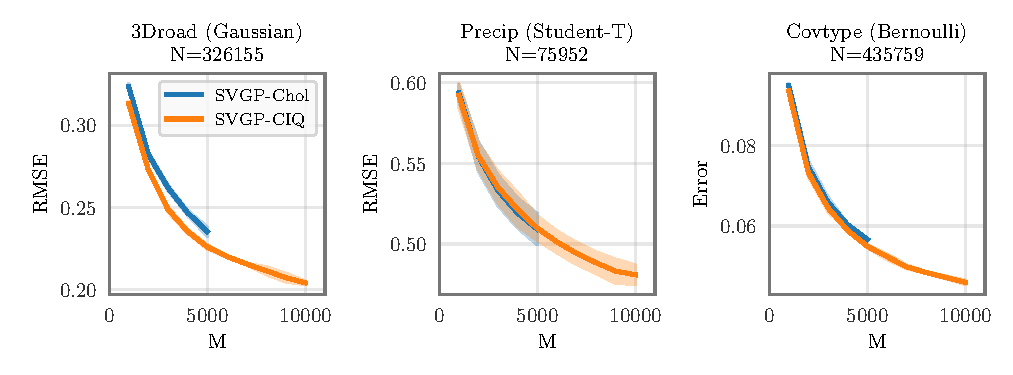
\includegraphics[width=\linewidth]{figures/variational_error.pdf}
  \caption[RMSE comparison of Cholesky-whitened vs CIQ-whitened SVGP models.]{
    RMSE comparison of Cholesky-whitened vs CIQ-whitened SVGP models.
    {\bf Left:} 3DRoad dataset ($N=326155, D=2$, Gaussian likelihood).
    {\bf Middle:} Precipitation dataset ($N=75952, D=3$, Student-T likelihood).
    {\bf Right:} CoverType dataset ($N=435759, D=54$, Bernoulli likelihood).
    NLL improves with more inducing points ($M$), and Cholesky and CIQ models have similar performance.
    However CIQ scales to larger values of $M$.
  }
  \label{fig:variational_error}
\end{figure}

\chapter{Full GPyTorch Code Examples}

The following are code examples for training and evaluating GPyTorch models.\footnote{
  Tested against GPyTorch v1.1---\gp{TODO: url}.
}
We include examples for a standard GP (with no approximations/exploitable structure) and a multitask GP.
Both models can be modified to use scalable methods by changing the {\tt covar\_module} (i.e. kernel).



\section{Standard GP Regression}
\label{app:standard_gp_example}

Here we train a standard GP with a {\tt RBFKernel}.
As described in \cref{sec:programmability}, each kernel object outputs a {\tt LazyTensor} object, which defines its own {\tt \_matmul($\cdot$)} function.
If the kernel has exploitable structure---e.g.
%
\begin{itemize}
  \item {\tt LinearKernel} for Bayesian linear regression,
  \item {\tt GridInterpolationKernel} wrapping a {\tt RBFKernel} for KISS-GP,
\end{itemize}
%
then the kernel will output the appropriate {\tt LazyTensor} subclass with a structure-exploiting {\tt \_matmul($\cdot$)} function for use with the mBCG algorithm.

\longcodetrue
\begin{minted}{python3}
import math
import torch
import gpytorch
from matplotlib import pyplot as plt

"""
Training data is 100 points in [0,1] inclusive regularly spaced
True function is sin(2*pi*x) with Gaussian noise
"""
train_x = torch.linspace(0, 1, 100)
train_y = torch.sin(train_x * (2 * math.pi)) + \
    torch.randn(train_x.size()) * math.sqrt(0.04)

"""
Now we define a class for basic GP models
"""
class ExactGPModel(gpytorch.models.ExactGP):
    def __init__(self, train_x, train_y, likelihood):
        super(ExactGPModel, self).__init__(
            train_x, train_y, likelihood
        )
        self.mean_module = gpytorch.means.ZeroMean()
        # We can implement specialty models by replacing
        # this kernel (e.g. LinearKernel.)
        # Each kernel uses a differen LazyTensor under the hood.
        self.covar_module = gpytorch.kernels.ScaleKernel(
            gpytorch.kernels.RBFKernel()
        )
        # To implement KISS-GP, wrap this kernel inside al
        # gpytorch.kernels.GridInterpolationKernel

    def forward(self, x):
        mean_x = self.mean_module(x)
        # Our kernel module returns a NonLazyTensor object.
        # If we were to replace it with a LinearKernel,
        # the output would be a RootLazyTensor
        covar_x = self.covar_module(x)
        return gpytorch.distributions.MultivariateNormal(
            mean_x, covar_x
        )

"""
Create an instance of our model and likelihood
"""
likelihood = gpytorch.likelihoods.GaussianLikelihood()
model = ExactGPModel(train_x, train_y, likelihood)

"""
A basic training loop.
The GPyTorch objects in this loop use BBMM under the hood.
"""
optimizer = torch.optim.Adam(model.parameters(), lr=0.01)

# "Loss" for GPs - the marginal log likelihood
# Calling this funcition uses BBMM to compute the marginal log
# likelihood and its derivative
mll = gpytorch.mlls.ExactMarginalLogLikelihood(likelihood, model)

# Training loop
model.train()
for i in range(100):
    optimizer.zero_grad()
    loss = -mll(model(train_x), train_y)
    loss.backward()
    optimizer.step()

"""
Making predictions.
We will use LOVE to for fast variances
"""
model.eval()
likelihood.eval()
# The fast_pred_var context manager turns on LOVE variances
with torch.no_grad(), gpytorch.settings.fast_pred_var():
    test_x = torch.linspace(0, 1, 51)
    pred = likelihood(model(test_x))
    # Get mean prediction
    mean = pred.mean
    # Get upper and lower confidence bounds
    lower, upper = pred.confidence_region()

"""
Plotting the model fit
"""
f, ax = plt.subplots(1, 1, figsize=(4, 3))
# Plot training data as black stars
ax.plot(train_x.numpy(), train_y.numpy(), "k*")
# Plot prediction
ax.plot(test_x.numpy(), mean.numpy(), "b")
ax.fill_between(
  test_x.numpy(), lower.numpy(), upper.numpy(), alpha=0.5
)
ax.set(ylim=[-3, 3], xlabel="x",  ylabel="y")
ax.legend(["Observed Data", "Mean", "Confidence"])
f.show()
\end{minted}
\longcodefalse

\begin{figure}[ht!]
  \centering
  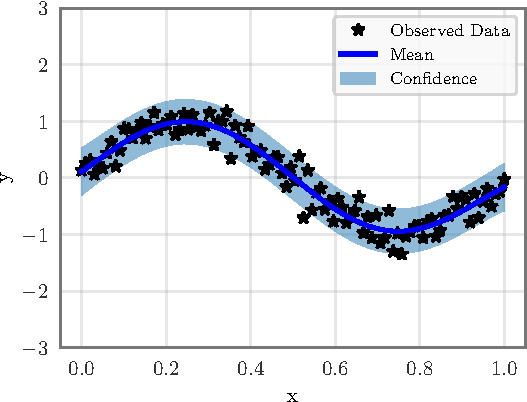
\includegraphics[width=0.5\linewidth]{figures/example_gpytorch_plot.pdf}
  \caption{
    Output plot from GPyTorch code example for standard GPs.
  }
  \label{fig:example_gpytorch_plot}
\end{figure}







\section{Multitask GP Regression}
\label{app:multitask_gp_example}

To demonstrate the modularity afforded by BBMM, we also include a code example of a multitask GP model.
What's notable is that this code example is essentially the same as the standard GP code example.
The only major difference is the kernel module ({\tt MultitaskKernel}),
which uses the ({\tt KroneckerProductLazyTensor}) under the hood for efficient inference.

\longcodetrue
\begin{minted}{python3}
import math
import torch
import gpytorch
from matplotlib import pyplot as plt

"""
Training data is 100 points in [0,1] inclusive regularly spaced
We train two outputs: a sin function and a cos function
    with Gaussian noise
"""
train_x = torch.linspace(0, 1, 100)
train_y = torch.stack([
    torch.sin(train_x * (2 * math.pi)),
    torch.cos(train_x * (2 * math.pi))
], -1)
train_y += torch.randn_like(train_y) * 0.2

"""
Now we define a class for multitask GP models
"""
class MultitaskGPModel(gpytorch.models.ExactGP):
    def __init__(self, train_x, train_y, likelihood):
        super(MultitaskGPModel, self).__init__(
            train_x, train_y, likelihood
        )
        self.mean_module = gpytorch.means.MultitaskMean(
            gpytorch.means.ZeroMean(), num_tasks=2
        )
        self.covar_module = gpytorch.kernels.MultitaskKernel(
            gpytorch.kernels.RBFKernel(), num_tasks=2, rank=1
        )

    def forward(self, x):
        mean_x = self.mean_module(x)
        covar_x = self.covar_module(x)
        return gpytorch.distributions.MultitaskMultivariateNormal(
            mean_x, covar_x
        )

"""
Create an instance of our model and likelihood
This example uses a MultitaskGaussianLikelihood to have seperate
    observation noise for each task.
"""
likelihood = gpytorch.likelihoods.MultitaskGaussianLikelihood(
    num_tasks=2
)
model = MultitaskGPModel(train_x, train_y, likelihood)


"""
Training with BBMM.
"""
optimizer = torch.optim.Adam(model.parameters(), lr=0.1)
mll = gpytorch.mlls.ExactMarginalLogLikelihood(likelihood, model)

model.train()
for i in range(100):
    optimizer.zero_grad()
    loss = -mll(model(train_x), train_y)
    loss.backward()
    optimizer.step()

"""
Making predictions with LOVE.
"""
model.eval()
likelihood.eval()
with torch.no_grad(), gpytorch.settings.fast_pred_var():
    test_x = torch.linspace(0, 1, 51)
    pred = likelihood(model(test_x))
    mean = pred.mean
    lower, upper = pred.confidence_region()


"""
Plotting the model fit
"""
f, (y1_ax, y2_ax) = plt.subplots(1, 2, figsize=(8, 3))
# Plot training data as black stars
y1_ax.plot(
    train_x.detach().numpy(), train_y[:, 0].detach().numpy(),
    "k*"
)
y2_ax.plot(
    train_x.detach().numpy(), train_y[:, 1].detach().numpy(),
    "k*"
)
# Plot predictions
y1_ax.plot(test_x.numpy(), mean[:, 0].numpy(), "b")
y2_ax.plot(test_x.numpy(), mean[:, 1].numpy(), "b")
# Shade in confidence
y1_ax.fill_between(
    test_x.numpy(), lower[:, 0].numpy(), upper[:, 0].numpy(),
    alpha=0.5
)
y2_ax.fill_between(
    test_x.numpy(), lower[:, 1].numpy(), upper[:, 1].numpy(),
    alpha=0.5
)
# Legend and axes
y1_ax.legend(["Observed Data", "Mean", "Confidence"])
y1_ax.set(ylim=[-3, 3], xlabel="x",  ylabel="y1")
y2_ax.set(ylim=[-3, 3], xlabel="x",  ylabel="y2")
f.show()
\end{minted}
\longcodefalse

\begin{figure}[ht!]
  \centering
  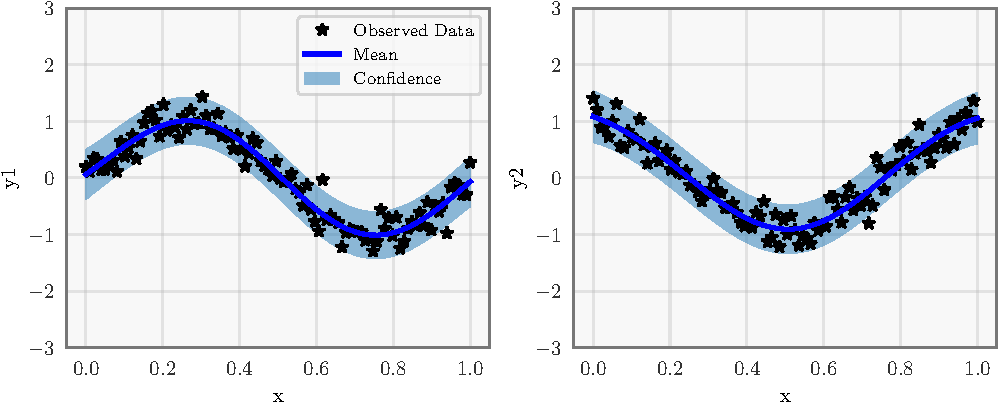
\includegraphics[width=\linewidth]{figures/example_gpytorch_plot_multitask.pdf}
  \caption{
    Output plot from GPyTorch code example for multitask GPs.
  }
  \label{fig:example_gpytorch_plot_multitask}
\end{figure}


\addcontentsline{toc}{chapter}{Bibliography}
\bibliography{gpleiss_thesis}



\end{document}
